%% Submitted to: 
%https://www.sciencedirect.com/journal/results-in-engineering

\documentclass[final,5p,times,twocolumn]{elsarticle}

\usepackage[numbers]{natbib}

%%%Author macros
\def\tsc#1{\csdef{#1}{\textsc{\lowercase{#1}}\xspace}}
\tsc{WGM}
\tsc{QE}
\tsc{EP}
\tsc{PMS}
\tsc{BEC}
\tsc{DE}
%%%
\usepackage{caption}

\usepackage{float}
\usepackage{amssymb,amsmath}
\usepackage{url}
\usepackage{xcolor}
\usepackage{bm}
\usepackage{placeins}
\usepackage{hyperref}
\usepackage{longtable} 
\usepackage[capitalise]{cleveref}
\usepackage{pifont}
\usepackage{lineno}
\usepackage{placeins}

\newcommand{\cmark}{\ding{51}}
\newcommand{\xmark}{\ding{55}}

\usepackage{array}
\newcolumntype{C}[1]{>{\centering\let\newline\\\arraybackslash\hspace{0pt}}m{#1}}


\usepackage{tikz}
\usetikzlibrary{shapes.geometric, arrows.meta, positioning, calc, fit, backgrounds, decorations.pathmorphing, patterns}
  

\definecolor{inputgreen}{RGB}{230, 245, 230} % Green for definitions
\definecolor{processblue}{RGB}{230, 245, 255} % Blue for physics/simulation
\definecolor{outputorange}{RGB}{255, 245, 230} % Orange for final data

%%Defining some useful variables 
\providecommand{\ve}[1]{{\bm{#1}}}
\providecommand{\mat}[1]{{\bm{#1}}} 
\providecommand{\var}[1]

\DeclareMathOperator{\subconj}{\negthinspace\subset\negthinspace }
\DeclareMathOperator{\en}{\!\,\in\!\,}
\DeclareMathOperator{\igual}{\!\,=\!\,}
\DeclareMathOperator{\dist}{\operatorname{d}}
\DeclareMathOperator{\xx}{\negthickspace\times\negthickspace}
\providecommand{\s}[1]{\negthinspace#1\negthinspace}

\begin{document}

\newcommand{\Real}{\mathbb{R}}
\newcommand{\N}{\mathbb{N}}
\newcommand{\Z}{\mathbb{Z}}
\newcommand{\X}{\mathcal{X}}
\newcommand{\Y}{\mathcal{Y}}
\newcommand{\boldV}{\mathbf{V}}
\newcommand{\dataset}{{\cal D}}
\newcommand{\gauss}{\mathcal{N}} 

\providecommand{\ch}[1]{\textcolor{blue}{#1}}

\let\WriteBookmarks\relax
\def\floatpagepagefraction{1}
\def\textpagefraction{.001}

%% Journal name (optional)
\journal{Results in Engineering}

\begin{frontmatter}


\title{Regression-Based Explainable Deep Learning for Estimating Hamiltonian Parameters from Magnetic Nanodot Images}

%% Authors and addresses
\author[unal]{Juan Sebasti\'an M\'endez-Rond\'on}
\ead{jumendezro@unal.edu.co}

\author[unal]{Mar\'ia Isabel Garc\'ia-Quimbayo}
\ead{migarciaq@unal.edu.co}

\author[unal]{Andr\'es Marino \'Alvarez-Meza\corref{cor1}}
\ead{amalvarezme@unal.edu.co}

\author[unal1]{Jorge Iv\'an Montes-Monsalve}
\ead{jimontesm@unal.edu.co}

\author[uam]{Jose Dar\'io Agudelo-Giraldo}
\ead{josed.agudelog@autonoma.edu.co}

\address[unal]{AI-Lab, Signal Processing and Recognition Group, Universidad Nacional de Colombia, Sede Manizales, 170003 Manizales, Colombia}

\address[unal1]{Direcci\'on Acad\'emica, Universidad Nacional de Colombia, Sede de La Paz, 202010 La Paz, Colombia}

\address[uam]{Grupo de Investigaci\'on en F\'isica y Matem\'aticas con \'Enfasis en la Formaci\'on de Ingenieros, Departamento de F\'isica y Matem\'aticas, Facultad de Ingenier\'ia, Universidad Aut\'onoma de Manizales, Antigua Estaci\'on del Ferrocarril, 170002  Manizales, Colombia}


\cortext[cor1]{amalvarezme@unal.edu.co}


\begin{abstract}
In magnetic nanodots, the stability of emergent topological textures is governed by an energetic competition described by the extended Heisenberg Hamiltonian, involving symmetric exchange, the Dzyaloshinskii–Moriya interaction (DMI), magnetocrystalline anisotropy, and the Zeeman field. Recovering these atomistic parameters from two-dimensional magnetic domain images is a severely ill-posed inverse problem, since distinct parameter combinations yield states with nearly indistinguishable free energies. Empirical fitting and simulation-based searches struggle to discriminate among competing solutions, while standard deep learning regressors collapse the multimodal inverse landscape into opaque, oversmoothed estimates. We propose an inherently explainable regression framework that couples Metropolis–Hastings Monte Carlo sampling with simulated annealing, used to generate thermodynamically relaxed magnetization fields, to convolutional and Vision Transformer architectures trained to recover eight Hamiltonian parameters. Interpretability is delivered by Regression Activation Maps (RAMs), a novel attribution method extending gradient-based saliency to continuous physical targets. On $218{,}256$ simulated configurations, the framework predicts the annealing temperature, second-shell exchange constant, and DMI strength with $R^2$ of $0.91$, $0.93$, and $0.97$. Unsupervised clustering of the latent space recovers four magnetic phases without supervision, and RAMs isolate chiral domain walls and skyrmion cores as the textures driving predictions, establishing a traceable link between atomistic design parameters and observable spin textures.
\end{abstract}

%%Graphical abstract
\begin{graphicalabstract}
\begin{figure}[h]
    \centering
    \resizebox{\linewidth}{!}{
    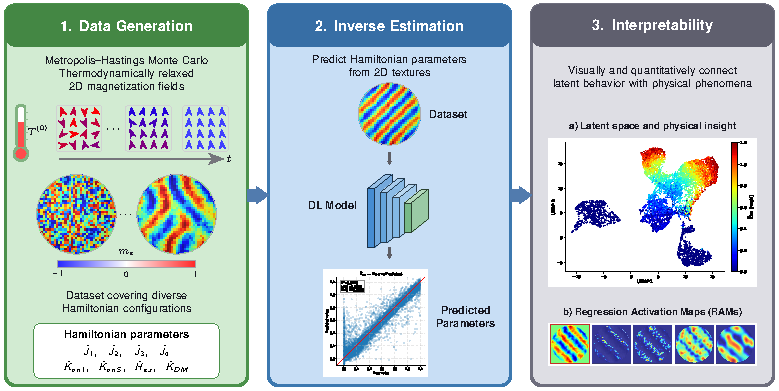
\includegraphics{graphical}}
    \label{fig:graphical_abstract}
\end{figure}
\end{graphicalabstract}



%%Research highlights

\begin{highlights}
\item Atomistic Hamiltonian generates relaxed 2D magnetic domain images for training.
\item Deep learning regression recovers Hamiltonian parameters from nanodot images.
\item Regression Activation Maps explain continuous prediction errors spatially.
\item Framework isolates degenerate textures linking black-box AI to magnetic physics.
\end{highlights}




\begin{keyword}
Explainable AI \sep Magnetic Nanodots \sep Hamiltonian Parameters \sep Regression Activation Maps \sep Deep Learning
\end{keyword}

\end{frontmatter}

\linenumbers


\section{Introduction}\label{sec:intro}

%nanoscale motivation and structures: helical, labyrinth and skyrmion
Understanding and controlling magnetic behavior at the nanometric scale is a central challenge in modern condensed matter physics and materials engineering~\cite{heinrich2021quantum}. This capability is particularly relevant to the development of spintronic devices, ultrahigh-density magnetic memories, and neuromorphic computing platforms based on topological magnetic textures~\cite{wang2022fundamental, fert2024electrical}. At such length scales, surface effects, geometric confinement, and energy quantization substantially modify magnetic properties relative to the bulk~\cite{issa2013magnetic}. The resulting enhancement of surface anisotropy, structural imperfections, and thermal fluctuations strongly affects the stability and dynamics of spin configurations~\cite{charalampidis2023metadynamics}. These effects give rise to emergent collective states—including ferromagnetic, helical, labyrinthine, and skyrmionic textures~\cite{yua2017magnetic, birch2020real, yu2021magnetic, zhang2023magnetic}—whose stability is governed by the interplay of competing microscopic interactions~\cite{tokura2020magnetic}. In this context, magnetic nanodots constitute an ideal model platform, as their lateral confinement favors the formation of single-domain states, vortices, and skyrmion-like configurations controlled by the balance among symmetric exchange, magnetic anisotropy, DMI, and external magnetic fields~\cite{zelent2023stabilization, rohart2013skyrmion}. Therefore, inferring these underlying physical parameters directly from magnetic domain images has become a critical inverse problem for the rational engineering of functional magnetic materials~\cite{kong2023quantifying}.

%hammiltonian and ill conditioned problem (degenerecy)
Within this framework, atomistic Hamiltonian-based modeling constitutes the most rigorous description of the discrete spin interactions, localized dynamics, and boundary effects that dominate nanoscale magnetic systems. Unlike continuum micromagnetic models, which can mask essential surface and finite-size contributions, the extended Heisenberg Hamiltonian explicitly captures the atomistic interactions responsible for stabilizing complex topological textures in magnetic nanodots~\cite{evans2014atomistic}. In its general form, the Hamiltonian includes several competing terms: the symmetric exchange interaction ($\tilde{J}$ [meV]), which promotes collinear alignment; the DMI ($\tilde{D}$ [meV]), which favors chiral and non-collinear spin textures; the magnetocrystalline anisotropy ($\tilde{K}$ [meV]), which selects preferred crystallographic orientations; and the Zeeman coupling to an external magnetic field ($\tilde{H}$ [meV])~\cite{aldarawsheh2023intrinsic}. The competition among these contributions generates a highly multimodal energy landscape~\cite{tokura2020magnetic,finocchio2016magnetic}, in which physically distinct parameter sets may produce spin states with nearly indistinguishable free energies. This degeneracy can lead to the coexistence of helical, skyrmion-like, and other metastable textures~\cite{back20202020, he2023ferroelectrically}, thereby rendering the inverse estimation of Hamiltonian parameters from two-dimensional magnetic domain images intrinsically ill-conditioned and structurally ambiguous~\cite{murakami2022inverse, kwon2020magnetic}.

% SOTA 1: Experimental and simulation limitations
The intrinsic ambiguity of the inverse problem is further exacerbated by the limitations of current experimental and analytical methodologies. Although advanced imaging techniques, including magnetic force microscopy, Lorentz transmission electron microscopy, and spin-polarized scanning tunneling microscopy~\cite{nguyen2022cooperative}, enable high-resolution visualization of magnetic textures, they typically provide indirect or transformed measurements that are subject to modality-dependent distortions, noise, and finite spatial resolution~\cite{zhao2025overview, gaida2023lorentz}. In practice, parameter estimation therefore relies heavily on empirical fitting or on comparison with synthetic magnetic configurations generated by atomistic spin simulations or continuum micromagnetic models~\cite{d2023micromagnetic, lepadatu2021micromagnetic}. Yet similarity measures defined in image space—such as mean squared error or structural similarity—are often inadequate for resolving topologically distinct states, since they primarily quantify visual resemblance rather than physical equivalence. Consequently, the optimization process remains structurally ambiguous, and substantially different Hamiltonian parameter sets may produce magnetic domain patterns that are visually indistinguishable ~\cite{yin2023computational, karnatov2025analysis}.

% SOTA 2: Deep Learning & Interpretability challenges
To circumvent the prohibitive cost of iterative simulation-based optimization, recent efforts have reformulated this inverse problem as a data-driven learning task using deep neural architectures~\cite{lee2024deep}. Although supervised regression models allow fast parameter inference, they generally impose an implicit one-to-one mapping and therefore tend to collapse the intrinsic multimodality of degenerate magnetic systems into oversmoothed point predictions~\cite{chen2024data}. Methods designed to explicitly capture this uncertainty—such as Bayesian inference, diffusion models, cycle-consistent networks, and physics-informed neural networks—offer improved representational flexibility, but often introduce substantial computational overhead and pronounced optimization stiffness~\cite{lan2022scaling, huang2023cycle, baldan2023physics}. Beyond these computational challenges, a central limitation remains their opacity. In strongly degenerate parameter spaces, conventional black-box models offer little or no mechanistic understanding of how localized spatial features contribute to the inferred Hamiltonian parameters~\cite{wang2021learning, vcadevz2026neural}. Moreover, although gradient-based attribution tools such as class activation maps are widely used in classification, analogous interpretability methods for continuous regression in highly multimodal physical systems remain underdeveloped~\cite{he2022survey}. This interpretability gap restricts the physical traceability required for robust and scientifically meaningful machine-learning-based inference.

\ch{Recent advances have demonstrated the immense potential of deep learning in resolving the inverse problem of magnetic Hamiltonian parameter estimation from domain images. For example, Kwon \textit{et al.} \cite{kwon2020magnetic} employed ResNet architectures to estimate Dzyaloshinskii-Moriya, anisotropy, and dipolar interactions from Monte Carlo-simulated spin configurations, while Kong \textit{et al.} \cite{kong2023quantifying} utilized customized convolutional neural networks to extract exchange stiffness, effective anisotropy, and interfacial DMI from micromagnetic simulations. More recently, Lee \textit{et al.} \cite{lee2024deep} demonstrated the applicability of fully connected networks for estimating interlayer and intralayer interactions in twisted van der Waals magnets. Despite their impressive predictive accuracy, these pioneering approaches predominantly treat the neural network as a ``black box.'' Specifically, while some works analyze intermediate feature maps \cite{kong2023quantifying} or perform statistical error analysis \cite{kwon2020magnetic, lee2024deep}, they lack spatially resolved attribution mechanisms to explicitly identify which morphological features of the spin textures drive specific parameter predictions. Furthermore, physical identifiability limits---such as degenerate spin configurations arising from competing symmetric interactions---are often encountered as empirical estimation errors rather than explicitly quantified boundaries. In this work, we address these critical gaps by integrating modern deep learning architectures (DenseNet121 and Vision Transformers) with a comprehensive Explainable AI (XAI) framework. By employing Regression Activation Mapping (RAM) and UMAP/HDBSCAN clustering, we provide direct spatial mappings of the network's attention on specific magnetic textures (e.g., skyrmions, domain walls). Moreover, we explicitly establish the physical identifiability boundaries for an 8-parameter extended Heisenberg Hamiltonian, thereby bridging the gap between high-throughput parameter regression and interpretable microscopic physics.}

% Proposal and Novelty
To address these limitations, we propose an inherently explainable framework grounded in an atomistic extended Heisenberg Hamiltonian. The proposed methodology explicitly captures the competition among symmetric exchange, DMI, magnetocrystalline anisotropy, and Zeeman coupling through Metropolis–Hastings Monte Carlo sampling and simulated annealing, enabling the generation of thermodynamically relaxed and highly accurate two-dimensional magnetization fields. These physically grounded data are subsequently integrated with a regression-based deep learning architecture for robust inverse estimation of the governing Hamiltonian parameters. The main contributions of this work are summarized as follows. First, we develop an atomistic Hamiltonian simulation framework based on the extended Heisenberg Hamiltonian, in which stochastic Monte Carlo sampling and simulated annealing are used to generate thermodynamically relaxed two-dimensional magnetization images and to establish an explicit correspondence between physical parameters and their associated topological magnetic states. Second, we integrate advanced convolutional neural networks and vision transformer architectures into a generalized regression framework for the robust prediction of fundamental Hamiltonian parameters from magnetic domain images. Third, we introduce RAMs, a novel interpretability framework that extends gradient-based activation mapping to continuous-valued physical targets, thereby providing both visual and quantitative insight into the relationship between the network’s latent representations and the underlying magnetic phenomena. Finally, we demonstrate that RAMs can isolate degenerate magnetic textures, such as chiral domain walls and skyrmions, that most strongly govern the prediction of specific Hamiltonian parameters, thus providing a physically traceable alternative to conventional deterministic models whose predictive mechanisms remain opaque.

% Experiments & Results Summary
To assess the effectiveness of the proposed framework, extensive experiments were performed using a custom-generated dataset of simulated magnetic domain images covering a broad range of Hamiltonian parameter configurations. The obtained results indicate that the proposed method enables accurate inverse prediction of key magnetic parameters, with the DenseNet121 architecture achieving the strongest overall performance among the tested models. In particular, the framework shows high predictive capability for the DMI and symmetric exchange parameters. Moreover, the qualitative and quantitative analyses based on RAMs indicate that the learned representations are associated with physically relevant spin topologies rather than dataset-specific noise or superficial correlations, thereby strengthening the interpretability and reliability of the proposed approach. The remainder of the paper is organized as follows. Section~\ref{sec:related} presents the related work. Section~\ref{sec:materials} details the materials and methods. Section~\ref{sec:experiments} describes the experimental setup. Section~\ref{sec:results_dis} presents and discusses the results. Finally, Section~\ref{sec:conclusions} concludes the paper and highlights future research directions.

\section{Related Work}\label{sec:related}

%Parameter Estimation in Nanoscale Magnetism
The inverse estimation of Hamiltonian parameters from magnetic domain configurations is widely recognized as a highly challenging problem due to the complex, nonlinear relationship between physical interactions and observable spin textures. From an experimental standpoint, researchers heavily rely on advanced indirect imaging techniques such as magnetic force microscopy, Lorentz transmission electron microscopy, and spin-polarized scanning tunneling microscopy~\cite{nguyen2022cooperative}. While these modalities enable high-resolution visualization of magnetic domains, they inherently capture transformed or partial projections of the underlying three-dimensional spin configurations. Because each technique is governed by distinct physical interaction principles, experimental observations are frequently contaminated by modality-specific distortions, finite spatial resolution limits, and heterogeneous noise, making direct inversion from these measurements generally infeasible~\cite{zhao2025overview, gaida2023lorentz}. 

%simulation methods
Consequently, practical parameter estimation heavily depends on empirical fitting or direct comparison with synthetic data generated through numerical simulations~\cite{zeng2022direct, altaf2024applications}. Computationally, the problem is most commonly addressed using physics-based forward simulations, specifically atomistic spin models governed by the extended Heisenberg Hamiltonian and continuum micromagnetic models~\cite{d2023micromagnetic, lepadatu2021micromagnetic, silva2024three}. However, attempting to optimize the inverse mapping by minimizing pixel-level discrepancy functions—such as Mean Squared Error or Mean Absolute Error—frequently fails to capture physically meaningful topological differences or vital spin interactions~\cite{mongwe2021adaptive, talapatra2022understanding}. Even structural metrics like the Structural Similarity Index fall short in this regard~\cite{karnatov2025analysis}. Ultimately, because the comparison between simulated and experimental data occurs strictly in the image space rather than the parameter space, the optimization landscape becomes highly ambiguous, allowing disparate parameter configurations to yield visually identical domain patterns~\cite{yin2023computational}.

%Deep Learning Architectures for Inverse Parameter Inference
To bypass the computationally prohibitive nature of iterative simulation-based optimization, recent advances have increasingly framed the inverse problem as a data-driven mapping utilizing deep learning architectures~\cite{lee2024deep}. The most prevalent approach employs supervised regression models, including convolutional neural networks and transformer-based architectures, to approximate this mapping deterministically. While these models offer rapid inference and scalability, they inherently assume a one-to-one mapping between images and parameters. In highly degenerate magnetic systems, this assumption causes the models to collapse the intrinsic multimodality of the parameter space into a single, often smoothed, point estimate, rendering them highly sensitive to dataset bias and sim-to-real mismatch~\cite{chen2024data}. 

%Bayesian methods
To explicitly model uncertainty and capture this multimodality, probabilistic frameworks such as Bayesian inference methods, conditional variational autoencoders, and diffusion models have been introduced~\cite{lan2022scaling, liu2026bayesian, zhao2023generative, shmakov2023end}. Despite their theoretical flexibility in sampling multiple plausible configurations, these generative and Bayesian approaches suffer from immense computational overhead, unstable training dynamics, and a distinct lack of explicit physical guarantees. In parallel, cycle-consistent frameworks and Physics-Informed Neural Networks attempt to constrain the solution space by enforcing coherence between forward and inverse mappings, or by directly embedding thermodynamic penalties into the loss function~\cite{huang2023cycle, sui2026cyclemamba, baldan2023physics}. While physically plausible, these hybrid models introduce severe optimization stiffness and rely fundamentally on the accuracy of the underlying forward surrogate, which can dangerously propagate errors within strongly degenerate spin regimes.

%Explainability and Interpretability in Physical Machine Learning
Despite the growing predictive capabilities of advanced deep neural networks, their fundamental opacity remains a critical barrier to their widespread adoption in condensed matter physics. In the context of nanoscale magnetism, the delicate energetic competition among the exchange interaction, the DMI, and magnetocrystalline anisotropy creates a densely degenerate parameter space where multiple physical configurations present nearly identical free energies~\cite{vcadevz2026neural, will2021application}. Traditional black-box deep learning architectures provide no mechanistic insight into how specific spatial features within a magnetic domain image correlate with the predicted Hamiltonian constants~\cite{wang2021learning, sridharan2022modern}. This lack of interpretability prevents researchers from distinguishing whether a model has genuinely captured the underlying physical laws or merely memorized superficial dataset artifacts. While gradient-based attribution methods like Class Activation Maps have been widely adopted for discrete classification tasks, interpreting continuous regression outputs in highly multimodal physical systems remains largely underexplored~\cite{he2022survey}. The inability to spatially trace and quantify the sources of prediction errors restricts the scientific traceability of these models, underscoring an urgent necessity for architectures that inherently couple high predictive accuracy with transparent, physics-informed spatial interpretations.

%novelty
To overcome the limitations, our methodology is fundamentally grounded in a rigorous atomistic extended Heisenberg Hamiltonian framework. By explicitly modeling the delicate energetic competition among symmetric exchange, DMI, magnetocrystalline anisotropy, and Zeeman coupling through Metropolis-Hastings Monte Carlo sampling and simulated annealing, we computationally stabilize and extract highly accurate, thermodynamically relaxed two-dimensional spatial magnetization fields. In contrast to prevalent black-box methodologies and computationally prohibitive probabilistic frameworks, we directly couple these physically exhaustive simulations with an inherently explainable, regression-based deep learning architecture explicitly designed for the rigorous inverse estimation of these governing parameters. By integrating advanced Convolutional and Visual Transformer networks, we robustly tackle the structural ambiguity of the inverse problem without sacrificing architectural transparency. Also, we introduce a RAMs, an interpretability approach that directly correlates localized spatial activations within the simulated magnetic domain visualizations to the absolute prediction error of the continuous physical variables. Unlike standard structural metrics or deterministic regression models that obscure the origin of their predictions, our method visually and quantitatively bridges the latent behavior of the neural network with the rigorously modeled phenomena. This enables the precise isolation of degenerate magnetic textures—such as chiral domain walls and skyrmions—that drive specific parameter estimations, establishing a highly reliable, transparent, and traceable pathway for analyzing complex nanoscale magnetic systems.



\section{Materials and Methods}\label{sec:materials}

\subsection{Atomistic Hamiltonian Framework}\label{sec:hamiltonian}

%hamiltonian fundaments
The theoretical foundation for modeling interacting magnetic dipole moments originates from the seminal formulations of Ernst Ising and Werner Heisenberg~\cite{agudelo2019study}. Ising introduced a one-dimensional statistical mechanics model wherein localized spins were heavily constrained to discrete, scalar states (i.e., rigidly pointing ``up'' or ``down''). While the Ising model provided early fundamental insights into macroscopic ferromagnetism and phase transitions, its strict uni-axial constraint renders it structurally insufficient for capturing the continuous rotational degrees of freedom required to model complex, multi-dimensional magnetic textures. This limitation was subsequently resolved by Heisenberg, who formulated a generalized model allowing spin vectors to vary continuously in three-dimensional space with rotational symmetry. While the foundational 
Heisenberg model successfully captures isotropic exchange driven by the Pauli exclusion principle, modern nanoscale applications—such as the study of magnetic vortices and topologically protected skyrmions in confined nanodot geometries—necessitate an extended 
approach~\cite{fert2024electrical}. This extended framework rigorously incorporates symmetry-breaking relativistic spin-orbit coupling effects, primarily the DMI and magnetocrystalline anisotropy, alongside standard Zeeman coupling~\cite{borisov2021heisenberg}.

%generalized formulation
Formally, let $\mathcal{V} = \{1, \dots, N\}$ denote the set of indices for the discrete magnetic lattice sites. The thermodynamic state of the system is characterized by the spatial distribution of localized magnetic moments, represented by the normalized spin vectors $\mathbf{s}_i \in \mathbb{R}^3$, subject to the constraint 
$\|\mathbf{s}_i\|_2 = 1$, for $i\in\mathcal{V}$. In a generalized theoretical context, all pairwise symmetric and antisymmetric interactions, as well as site-specific field and anisotropy alignments, can be collapsed into a unified geometric approach~\cite{moriya1960anisotropic,eriksson2017atomistic}. The total effective energy of the system $\mathcal{H}\in\mathbb{R}$ [meV] is thus defined by the following generalized quadratic form:

\begin{equation}\label{eq:GeneralizedHamiltonian}
\mathcal{H}\left(\mathbf{S}| \breve{\theta}\right) = 
- \sum_{i=1}^{N}\sum_{j\in \mathcal{N}(i)} 
    \langle \mathbf{s}_i, \tilde{\mathbf{M}}_{ij}\mathbf{s}_j \rangle
- \sum_{i=1}^{N} \langle\tilde{\mathbf{h}}_{i},\mathbf{s}_i\rangle 
- \sum_{i=1}^{N} \langle\mathbf{s}_i \tilde{\mathbf{K}}_i, 
    \mathbf{s}_i\rangle,
\end{equation}
where $\mathcal{N}(i)$ defines the set of interacting nearest neighbors for a given site $i$, and the matrix $\mathbf{S}\in\mathbb{R}^{N\times 3}$ 
gathers the continuous spin vectors across the lattice with 
$\mathbf{s}_i\in\mathbf{S}$. Here, 
$\breve{\theta}=\{\tilde{\mathbf{M}}_{ij},\tilde{\mathbf{h}}_{i},
\tilde{\mathbf{K}}_{i}\}$, where 
$\tilde{\mathbf{M}}_{ij} \in \mathbb{R}^{3 \times 3}$ represents the complete bilinear interaction matrix coupling neighboring spins, $\tilde{\mathbf{h}}_i \in \mathbb{R}^{3}$ accounts for linear external field interactions, and $\tilde{\mathbf{K}}_i \in \mathbb{R}^{3 \times 3}$ 
is the anisotropy tensor governing site-specific directional preferences.

%Decomposition and Factorization
Afterward, to recover the isolated physical phenomena and define an extended target scalar parameter space 
$\boldsymbol{\theta}=[\tilde{J}_1,\tilde{J}_2,\tilde{J}_3,\tilde{J}_4,
\tilde{D},\tilde{H},\tilde{K}_{an1},\tilde{K}_{anS}]$, the generalized matrices must be mathematically decomposed. By factorizing these parameters, we can map each matrix operation to its specific energetic contribution:

\begin{itemize}

    \item[--] \emph{Bilinear Coupling ($\tilde{\mathbf{M}}_{ij}$):} A 
    real square matrix can be separated into its symmetric and skew-symmetric components. Here, 
    $\tilde{\mathbf{M}}_{ij}$ is parameterized by factorizing the isotropic exchange scalar $\tilde{J}_r$ for the $r$-th neighbor shell and the DMI magnitude $\tilde{D}$ along a predefined spatial direction vector $\hat{\mathbf{d}}_{ij} \in \mathbb{R}^3$ 
    ($\|\hat{\mathbf{d}}_{ij}\|_2=1$), yielding:
    
    \begin{equation}\label{eq:MatrixDecomposition}
    \tilde{\mathbf{M}}_{ij}(\tilde{J}_r,\tilde{D}) = 
        \tilde{J}_r \mathbf{I} - \tilde{D} [\hat{\mathbf{d}}_{ij}]_{\times},
    \end{equation}
    where $\mathbf{I} \in \mathbb{R}^{3 \times 3}$ represents the identity matrix and 
    $[\hat{\mathbf{d}}_{ij}]_{\times} \in \mathbb{R}^{3 \times 3}$ denotes the skew-symmetric matrix representation of the cross-product. The symmetric exchange is modeled across four neighbor shells $r \in \{1,2,3,4\}$, where $\mathcal{N}_r(i)$ denotes the 
    set of neighbors at shell $r$ around site $i$, ordered by 
    increasing interatomic distance ($d_1 < d_2 < d_3 < d_4$). To resolve the fundamental scale ambiguity of the inverse problem---whereby multiplying all parameters by a common factor leaves the observable spin configuration unchanged---the first-shell exchange is fixed as the energy reference unit, $\tilde{J}_1\in \mathbb{R}$ in meV, while $\tilde{J}_2, \tilde{J}_3, \tilde{J}_4 \in \mathbb{R}$ are free parameters (also in meV). The DMI acts exclusively between first-shell neighbors and is therefore indexed only over $\mathcal{N}_1(i)$.

    \item[--] \emph{Zeeman Interaction ($\tilde{\mathbf{h}}_i$):} The linear field term is factorized by extracting the scalar field magnitude $\tilde{H}$ and the fixed normalized direction vector 
    $\hat{\mathbf{h}} = \hat{\mathbf{e}}_x,$ with 
    $\|\hat{\mathbf{e}}_x\|_2 = 1$, of the externally applied 
    magnetic field, yielding $\tilde{\mathbf{h}}_i = \tilde{H}\,\hat{\mathbf{e}}_x\in\mathbb{R}^3$. Fixing the field direction along $\hat{\mathbf{e}}_x$ eliminates the orientational degree of freedom of $\tilde{\mathbf{h}}_i$, ensuring that $\tilde{H}$ alone serves as the free parameter governing the Zeeman 
    contribution.

    \item[--] \emph{Magnetocrystalline Anisotropy 
    ($\tilde{\mathbf{K}}_i$):} Modeling cubic magnetocrystalline anisotropy requires factorizing a site-dependent scalar constant $\tilde{K}_i^{eff}$ to scale a quartic interaction. The principal crystallographic axes of the nanodot are defined by the orthonormal basis vectors $\mathbf{e}_{\hat{x}}, \mathbf{e}_{\hat{y}}, 
    \mathbf{e}_{\hat{z}} \in \mathbf{E}$, with $\mathbf{E} \in \mathbb{R}^{3 \times 3}$, and the directional cosines are given by $s_{im} = \langle \mathbf{e}_m,\mathbf{s}_i\rangle$ 
    ($\forall m\in\{\hat{x},\hat{y},\hat{z}\}$). Because atoms at the nanodot surface experience broken inversion symmetry---having fewer neighbors on the exterior side---their anisotropy differs fundamentally from that of interior atoms. The lattice is therefore partitioned into two disjoint subsets: the bulk region $\mathcal{V}_{bulk} \subset \mathcal{V}$, comprising interior sites with complete coordination shells, and the surface region 
    $\mathcal{V}_{surf} \subset \mathcal{V}$, comprising boundary sites exposed to the geometric confinement, with 
    $\mathcal{V}_{bulk} \cup \mathcal{V}_{surf} = \mathcal{V}$ and $\mathcal{V}_{bulk} \cap \mathcal{V}_{surf} = \emptyset$. This yields the site-dependent effective anisotropy constant:
    
    \begin{equation}\label{eq:AnisotropyEffective}
    \tilde{K}_i^{eff} = 
    \begin{cases}
        \tilde{K}_{an1} & \text{if } i \in \mathcal{V}_{bulk}, \\
        \tilde{K}_{anS} & \text{if } i \in \mathcal{V}_{surf},
    \end{cases}
    \end{equation}
    where $\tilde{K}_{an1}, \tilde{K}_{anS} \in \mathbb{R}$ are scalar constants measured in meV per atom~\cite{cullity2011introduction}.

\end{itemize}

%Explicit Formulation
Substituting these factorized relationships back into 
Equation~\ref{eq:GeneralizedHamiltonian} yields the following explicit formulation for the total extended Hamiltonian:

\begin{align}\label{eq:Hamiltonian}
\mathcal{H}\left(\mathbf{S}|\hat{\mathbf{d}}_{ij},\hat{\mathbf{e}}_x;
\boldsymbol{\theta}\right) = 
&- \sum_{r=1}^{4}\tilde{J}_r 
    \sum_{i=1}^{N}\sum_{j\in \mathcal{N}_r(i)} 
    \langle \mathbf{s}_i, \mathbf{s}_j \rangle \nonumber + \tilde{D} \sum_{i=1}^{N}\sum_{j\in \mathcal{N}_1(i)} 
    \langle \hat{\mathbf{d}}_{ij},(\mathbf{s}_i \times \mathbf{s}_j)
    \rangle \nonumber \\
&- \tilde{H} \sum_{i=1}^{N} 
    \langle \hat{\mathbf{e}}_x, \mathbf{s}_i \rangle \nonumber + \frac{1}{S_o^4}\sum_{i=1}^{N} \tilde{K}_i^{eff}
    \left(s_{i\hat{x}}^2 s_{i\hat{y}}^2 + 
          s_{i\hat{x}}^2 s_{i\hat{z}}^2 + 
          s_{i\hat{y}}^2 s_{i\hat{z}}^2\right),
\end{align}
with $\tilde{J}_1 = 1.0$~meV fixed as the energy reference unit. The cubic anisotropy form in the last term follows directly from expanding $\frac{1}{2}(1 - \|\mathbf{s}_i\mathbf{E}\|_4^4)$ under the $L_2$ normalization constraint $\|\mathbf{s}_i\|_2 = 1$, which 
yields $s_{i\hat{x}}^2 s_{i\hat{y}}^2 + s_{i\hat{y}}^2 
s_{i\hat{z}}^2 + s_{i\hat{z}}^2 s_{i\hat{x}}^2$, normalized by $S_o^4$ to maintain dimensional consistency across spin magnitudes.

%parameter interpretation
Physically, the extended parameter space $\boldsymbol{\theta}$ actively governs the competing energetic contributions that shape the magnetic energy landscape. Each $\tilde{J}_r$ dictates the collinear alignment tendency between spin pairs separated by the corresponding distance~\cite{coey2010magnetism}: positive values ($\tilde{J}_r > 0$) favor parallel, ferromagnetic 
alignment, while negative values ($\tilde{J}_r < 0$) drive 
antiparallel, antiferromagnetic order. This multi-shell formulation is essential in confined nanodot geometries, where longer-range exchange pathways--mediated through intermediate atomic orbitals--contribute non-negligibly to the global energetic competition and can selectively stabilize or destabilize complex topological textures beyond what first-shell interactions alone would predict~\cite{eriksson2017atomistic}. Among these constants, $\tilde{J}_1$ plays a privileged role: it 
corresponds to the strongest and most spatially direct exchange pathway, coupling each spin to its nearest neighbors in the cubic lattice and establishing the dominant energy scale of the magnetic system. For this reason, $\tilde{J}_1$ is fixed to $1.0$~meV throughout all simulations, serving as the absolute energy reference unit against which all remaining interaction strengths are expressed. The remaining constants $\tilde{J}_2$, $\tilde{J}_3$, and $\tilde{J}_4$ are free parameters whose magnitudes decay with increasing shell distance, consistent with the exponential attenuation of quantum mechanical exchange integrals with interatomic separation~\cite{coey2010magnetism}.

The DMI magnitude, represented by $\tilde{D}$, is responsible for driving chiral, non-collinear spin winding in systems exhibiting broken spatial inversion symmetry~\cite{fert2017magnetic}. By actively competing with the dominant first-shell exchange $\tilde{J}_1$, 
this antisymmetric contribution stabilizes complex topological textures, such as chiral domain walls and skyrmions. It acts exclusively between first-shell neighbors, as longer-range antisymmetric exchange pathways are negligibly small compared to the dominant spin-orbit coupling at nearest-neighbor interfaces. Measured in meV per interacting spin pair, its magnitude is fundamentally dependent on the strength of the spin-orbit coupling 
at the material's interfaces, with typical values spanning 
$[-0.5, 0.5]$~meV as a fraction of the first-shell exchange 
energy~\cite{fert2017magnetic}.

The Zeeman coupling energy, parameterized as $\tilde{H}$, quantifies the interaction between the localized atomic spins and the externally applied magnetic field~\cite{evans2014atomistic}. It systematically 
penalizes magnetic misalignment with the fixed crystallographic axis $\hat{\mathbf{e}}_x$, frequently serving as the primary thermodynamic driving force for macroscopic magnetic phase transitions. This 
parameter is expressed in meV per atom, mathematically representing the effective energy equivalence ($g\mu_B B$) that transitions a macroscopic magnetic field $B$ measured in Tesla into the atomistic energy regime. Its boundaries range from $0.0$~meV to approximately $2.0$~meV, directly correlating to laboratory-scale magnetic fields 
between $0$ and $10$~Tesla. Also, fixing the field direction along $\hat{\mathbf{e}}_x$ reduces the dimensionality of the inverse problem by eliminating the orientational degree of freedom of $\tilde{\mathbf{h}}_i$, ensuring that $\tilde{H}$ alone governs the Zeeman contribution as a single identifiable scalar.

Finally, the magnetocrystalline anisotropy encodes the intrinsic directional preference for magnetization relative to the underlying crystal lattice~\cite{cullity2011introduction}. Arising from 
relativistic spin-orbit coupling, this term rigorously establishes the energetically favorable (easy) and unfavorable (hard) crystallographic axes for spin orientation within the nanodot. Both constants are measured in meV per atom and represent a relatively subtle symmetry-breaking energy compared to the dominant isotropic 
exchange. The bulk anisotropy constant $\tilde{K}_{an1}$ governs interior lattice sites $i \in \mathcal{V}_{bulk}$, where each atom is fully coordinated by neighbors in all spatial directions, yielding a locally symmetric energetic environment. Its conventional boundaries range from roughly $0.001$~meV in soft bulk magnets to $1.0$~meV in 
highly anisotropic hard nanomaterials~\cite{cullity2011introduction}. The surface anisotropy constant $\tilde{K}_{anS}$, by contrast, 
governs boundary sites $i \in \mathcal{V}_{surf}$, where broken spatial inversion symmetry---arising from the absence of neighbors on the exterior side of the nanodot---produces an asymmetric local environment that intensifies the directional preference for spin orientation. Consequently, $|\tilde{K}_{anS}|$ is generally larger than $|\tilde{K}_{an1}|$, reflecting the enhanced symmetry-breaking at the nanodot boundary. This two-constant formulation is essential for accurately capturing the finite-size and surface-dominated effects that critically govern the stability of emergent topological textures 
in confined nanoscale geometries~\cite{fert2024electrical,borisov2021heisenberg}.

\subsection{Image-Based Dataset Generation From Monte Carlo Simulations}\label{sec:montecarlo_sim}

To accurately capture the physical thermodynamic behavior and algorithmically \ch{drive the system toward a low-energy, thermodynamically stable configuration} of the nanodot, thermal fluctuations must be formally introduced through the framework of statistical mechanics. While the atomistic Hamiltonian $\mathcal{H}$ rigorously defines the internal magnetic energy for a given spatial configuration of spins, it evaluates the system strictly as a frozen, zero-temperature snapshot. Hence, temperature is fundamentally a macroscopic parameter that governs the statistical distribution of the discrete magnetic microstates rather than acting as a localized interaction within the Hamiltonian. Consequently, temperature $T$ $[K]$ couples to the system via the Boltzmann distribution~\cite{eriksson2017atomistic}. Formally, a magnetic microstate $\mu$ represents a specific, instantaneous realization of the continuous spin matrix, denoted as $\mathbf{S}_\mu$. The total thermodynamic energy of this specific configuration is evaluated against the static environmental vectors and physical interaction strengths, such that $\mathcal{H}(\mu) \equiv \mathcal{H}\left(\mathbf{S}_\mu|\mathbf{\hat{d}}_{ij},\hat{\mathbf{h}},\mathbf{E};\boldsymbol{\theta}\right)$. At thermal equilibrium, the probability $P(\mu)$ of the system occupying this specific microstate is defined as:

\begin{equation}\label{eq:Boltzmann}
P(\mu) = \frac{1}{\mathcal{Z}} \exp\left(-\frac{\mathcal{H}(\mu)}{k_B T}\right),
\end{equation}
where $k_B$ is the Boltzmann constant (expressed in $\text{meV/K}$). The term $\mathcal{Z}$ represents the canonical partition function, which mathematically enforces probability normalization by summing over all valid spin configurations $\nu$ (i.e., all possible state matrices $\mathbf{S}_\nu$ strictly satisfying the geometric boundary constraint $\|\mathbf{s}_i\|_2 = 1$):

\begin{equation}\label{eq:PartitionFunction}
\mathcal{Z} = \sum_{\mathbf{S}_\nu} \exp\left(-\frac{\mathcal{H}\left(\mathbf{S}_\nu|\mathbf{\hat{d}}_{ij},\hat{\mathbf{h}},\mathbf{E};\boldsymbol{\theta}\right)}{k_B T}\right).
\end{equation}

In our computational framework, this thermodynamic distribution is actively sampled using the Metropolis-Hastings Monte Carlo algorithm combined with a simulated annealing protocol~\cite{landau2021guide}. This stochastic sampling ensures a rigorous exploration of the highly multimodal energy landscape characteristic of these degenerate magnetic systems. When a localized spin perturbation proposes a physical transition from the current microstate $\mu^{(t)}$ (characterized by $\mathbf{S}_{\mu^{(t)}}$) to a newly modified state $\mu^{(t+1)}$ (characterized by $\mathbf{S}_{\mu^{(t+1)}}$), the resulting change in the system's total energy is computed as the scalar difference $\Delta \mathcal{H} = \mathcal{H}(\mu^{(t+1)}) - \mathcal{H}(\mu^{(t)})$. To optimize computational efficiency, $\Delta \mathcal{H}$ is evaluated locally at the perturbed lattice site. The proposed state is subsequently accepted or rejected based on the precise transition probability:

\begin{equation}\label{eq:Metropolis}
P(\mu^{(t)} \rightarrow \mu^{(t+1)}) = \begin{cases}
1 & \text{if } \Delta \mathcal{H} < 0 \\
\exp\left(-\frac{\Delta \mathcal{H}}{k_B T^{(t)}}\right) & \text{if } \Delta \mathcal{H} \geq 0.
\end{cases}
\end{equation}

Physically, the instantaneous temperature parameter $T^{(t)}$ actively scales the energetic barriers within the system's vast topological energy landscape during the annealing process~\cite{landau2021guide}. At elevated temperatures, the available thermal energy $k_B T^{(t)}$ frequently exceeds local energy penalties ($\Delta \mathcal{H}$), allowing the simulation to accept thermodynamically unfavorable spin alignments. This thermal noise provides the critical kinetic mechanism required to break out of metastable, localized energy minima, such as misaligned ferromagnetic domains~\cite{desplat2018thermal}. As $T^{(t)}$ is systematically scaled down during the annealing procedure, the probability of accepting higher-energy configurations undergoes exponential decay. \ch{This controlled thermal relaxation drives the continuous spin vector field toward a low-energy, thermodynamically stable configuration consistent with the annealing schedule, promoting the stabilization of complex chiral skyrmion textures driven by the underlying DMI. We note that while simulated annealing with a finite cooling rate does not formally guarantee convergence to the absolute global minimum---particularly in DMI-driven systems where numerous metastable chiral states may coexist---the monotonic energy decrease observed across all simulated configurations (see Section~\ref{sec:results_dis}) provides empirical evidence of thorough thermodynamic relaxation within the sampled parameter space.}

Moreover, to ensure that each simulation consistently originates from a fully randomized paramagnetic phase regardless of the specific parameter configuration, the initial annealing temperature (i.e., $T^{(t)}$ at $t=0$) is established as an \textit{exchange-normalized initial temperature}. Consistent with foundational statistical mechanics~\cite{eriksson2017atomistic}, this starting temperature is dynamically rescaled in direct proportion to the dominant symmetric exchange energy ($\tilde{J}$). This energetic normalization guarantees that the initial thermal fluctuations are strictly sufficient to overcome the highest localized energetic barriers ($\Delta \mathcal{H}$) for that specific Hamiltonian. This effectively erases initial state bias and prevents the continuous spin vector field from prematurely collapsing into metastable local minima before the controlled cooling protocol begins.

To generate a robust and diverse dataset for deep learning evaluation, the magnetic parameters governing the Hamiltonian were systematically varied across the simulations. Key variables included the exchange interaction constant ($\tilde{J}$), the magnetocrystalline anisotropy ($\tilde{K}$), the external Zeeman field ($\tilde{H}$), and the DMI strength ($\tilde{D}$), alongside variations in the base initial temperature ($T^{(0)}$). Subsequently, the transformation of these raw, converged 3D spin states into normalized 2D image arrays followed a strict procedural pipeline:

\begin{itemize}
    \item[--] \emph{Geometry parsing:} Spatial coordinates defining the nanodot geometry (with a fixed disk radius and thickness as Magnetic Unit Cell (MUC) measure) were established using a binary circular lattice mask.
    \item[--] \emph{Spin state mapping:} The topological structure was projected into two dimensions by extracting the out-of-plane $s_z$ component of the continuous spin vectors ($\mathbf{s}_i$) across the valid lattice coordinates. 
    \item[--] \emph{Image rendering:} The isolated configurations were rasterized onto a fixed $\breve{H} \times \breve{W}$ pixel grid. A divergent red--blue colormap was utilized to strictly encode opposite spin polarities, visually capturing the chiral winding from the nanodot's core to its perimeter.
    \item[--] \emph{Preprocessing:} Pixel intensities corresponding to the $S_z$ magnitude were normalized to a strict interval $[0, 1]$ to ensure stable gradient flows during the deep learning optimization phase. To preserve the intrinsic physical symmetries and chiral handedness dictated by the DMI, no spatial augmentations (such as random rotations or structural flips) were applied to the dataset.
\end{itemize}

%dataset
Lastly, the simulation pipeline yields a comprehensive image-based dataset, formalized as $\mathcal{D} = \{\mathbf{X}_n, \boldsymbol{\theta}_n\}_{n=1}^{\breve{N}}$, which serves as the final collection of input-output pairs for the deep learning parameter estimation task. Each input tensor $\mathbf{X}_n \in [0,1]^{\breve{H} \times \breve{W}}$ encodes the two-dimensional spatial magnetization field (the normalized $s_z$ projection), while the corresponding target vector $\boldsymbol{\theta}_n \in \mathbb{R}^{\breve{P}}$ stores the $\breve{P}$-dimensional array of generating thermodynamic and Hamiltonian parameters (e.g., $\boldsymbol{\theta}_n = [T^{(0)}_n,\tilde{J}_{1n},\tilde{J}_{2n},\tilde{J}_{3n},\tilde{J}_{4n},\tilde{D_n},\tilde{H_n},\tilde{K}_{an1n},\tilde{K}_{anSn}]$). Figure~\ref{fig:methodology_flowchart} depicts the main flowchart of our image-based magnetic dataset generation approach.

\begin{figure*}[t!]
    \centering
    \resizebox{\linewidth}{!}{
    
    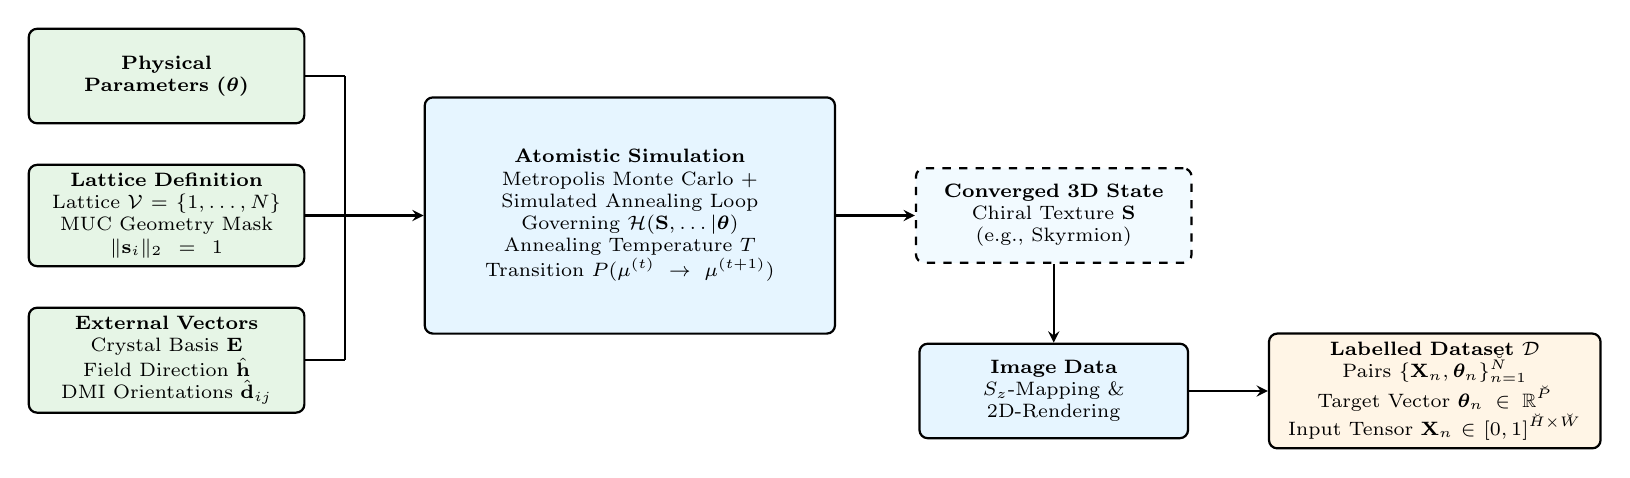
\begin{tikzpicture}[
        % --- TikZ Styles ---
        basebox/.style={
            draw, thick, minimum width=3.5cm, minimum height=1.2cm, 
            text width=3.2cm, align=center, font=\scriptsize, rounded corners=3pt,
            inner sep=3pt
        },
        inputbox/.style={basebox, fill=inputgreen},
        processbox/.style={basebox, fill=processblue},
        outputbox/.style={basebox, fill=outputorange},
        arrow/.style={thick, ->, >=stealth}
    ]

    % --- 1. INPUTS ---
    \node[inputbox] (params) {
        \textbf{Physical\\ Parameters ($\boldsymbol{\theta}$)}        
    };

    \node[inputbox, below=0.5cm of params] (lattice) {
        \textbf{Lattice Definition} \\
        Lattice $\mathcal{V}=\{1, \dots, N\}$ \\
        MUC Geometry Mask \\
        $\|\mathbf{s}_i\|_2 = 1$
    };

    \node[inputbox, below=0.5cm of lattice] (vectors) {
        \textbf{External Vectors} \\
        Crystal Basis $\mathbf{E}$ \\
        Field Direction $\hat{\mathbf{h}}$ \\
        DMI Orientations $\hat{\mathbf{d}}_{ij}$
    };

    % --- 2. SIMULATION ---
    \node[processbox, right=1.5cm of lattice, minimum height=3cm, text width=5cm] (mcsim) {
        \textbf{Atomistic Simulation} \\
        Metropolis Monte Carlo + Simulated Annealing Loop\\
        Governing $\mathcal{H}(\mathbf{S}, \dots | \boldsymbol{\theta})$ \\
        Annealing Temperature $T$\\
        Transition $P(\mu^{(t)} \to \mu^{(t+1)})$ 
    };

    \node[processbox, fill=processblue!50, dashed, right=1cm of mcsim] (topology) {
        \textbf{Converged 3D State} \\
        Chiral Texture $\mathbf{S}$\\
        (e.g., Skyrmion)
    };

    % --- 3. DATA GENERATION ---
    \node[processbox, below=1cm of topology,minimum width=3cm] (pipeline) {\textbf{Image Data}\\
    $S_z$-{Mapping} $\&$ 2D-Rendering
    };

    \node[outputbox, right=1cm of pipeline, minimum width=4.2cm, text width=4cm] (dataset) {
        \textbf{Labelled Dataset $\mathcal{D}$} \\
        Pairs $\{\mathbf{X}_n, \boldsymbol{\theta}_n\}_{n=1}^{\breve{N}}$ \\
        Target Vector $\boldsymbol{\theta}_n \in \mathbb{R}^{\breve{P}}$\\
        Input Tensor $\mathbf{X}_n \in [0,1]^{\breve{H} \times \breve{W}}$
    };

% --- CONNECTIONS ---
    
    % 1. Inputs to Simulation (Grouped 'Bus' Routing)
    % Draw horizontal lines out from top and bottom nodes
    \draw[thick] (params.east) -- ++(0.5,0) coordinate (bus_top);
    \draw[thick] (vectors.east) -- ++(0.5,0) coordinate (bus_bot);
    
    % Connect them with a vertical line
    \draw[thick] (bus_top) -- (bus_bot);
    
    % Draw the main arrow from the center node (intersecting the bus) to the simulation
    \draw[arrow] (lattice.east) -- (mcsim.west);
    
    % 2. Simulation to Pipeline to Output
    \draw[arrow] (mcsim.east) -- (topology.west);
    \draw[arrow] (topology.south) -- (pipeline.north);
    \draw[arrow] (pipeline.east) -- (dataset.west);

    \end{tikzpicture}}
 \caption{Main flowchart detailing the generation of the image-based magnetic dataset. The pipeline initializes with the foundational inputs (green), encompassing the Hamiltonian interaction parameters ($\boldsymbol{\theta}$), the discrete unit cell geometry, and the external directional vectors. These constraints govern the atomistic simulation (blue), which employs the Metropolis Monte Carlo algorithm coupled with simulated annealing to thermodynamically relax the system into a converged 3D topological state. Finally, the resulting continuous vector field is projected, rendered, and preprocessed (yellow) to formulate the labelled dataset $\mathcal{D}$, mapping 2D spatial magnetization images to their generating physical parameters.}
    \label{fig:methodology_flowchart}
\end{figure*}

\subsection{Deep Regression Framework for Hamiltonian Parameter Estimation}\label{sec:Deep_Learning}

The inverse estimation of the Hamiltonian parameters and thermodynamic state from magnetic domain images is formalized as a continuous mapping problem. Given the generated dataset $\mathcal{D}$, where $\mathbf{X}_n$ represents the normalized $s_z$ spatial magnetization field and $\boldsymbol{\theta}_n$ represents the vector of generating physical parameters, we aim to learn a parameterized non-linear mapping function $f_\Theta : \mathbb{R}^{\breve{H} \times \breve{W}} \rightarrow \mathbb{R}^{\breve{P}}$, to find the predicted parameters $\hat{\boldsymbol{\theta}}_n\in\mathbb{R}^{\breve{P}}.$

Here, $f_\Theta$ denotes a deep neural network architecture parameterized by a set of learnable weights and biases $\Theta$. The optimal parameter set $\hat{\Theta}$ is obtained by minimizing a continuous loss function over the training distribution~\cite{murphy2023probabilistic}:

\begin{equation}\label{eq:LossFunction}
\hat{\Theta} = \arg\min_{\Theta} \frac{1}{\breve{N}} \sum_{n=1}^{\breve{N}} \mathcal{L}\left(\boldsymbol{\theta}_n, f_\Theta(\mathbf{X}_n)\right),
\end{equation}
where $\mathcal{L}$ represents the chosen regression objective, typically the Mean Squared Error (MSE) or Huber loss, which mitigates the influence of outlier topological states during optimization. By minimizing this objective, the network intrinsically learns to untangle the highly multimodal spatial features mapping to the specific energetic balances of the extended Heisenberg Hamiltonian.

To achieve robust feature extraction across varying scales of magnetic textures (e.g., from localized domain walls to global skyrmion geometries), this framework evaluates four distinct, state-of-the-art deep learning architectures: ResNet50, DenseNet, Xception, and the Visual Transformer (ViT).

\begin{itemize}

\item[--] \emph{Residual Networks (ResNet50)}~\cite{koonce2021resnet}: Standard deep convolutional networks often suffer from the vanishing gradient problem as depth increases, hindering the learning of complex physical mappings. ResNet50 circumvents this by introducing shortcut connections that bypass multiple convolutional layers, directly propagating spatial information and gradients. Mathematically, if $\mathbf{x}$ is the input to a sequence of layers, and $\mathcal{F}(\mathbf{x}, \{\mathbf{W}_l\})$ represents the residual mapping to be learned (comprising convolutions, batch normalization, and ReLU activations) for the $l$-th layer, the output $\mathbf{y}$ of the residual block is defined as:

\begin{equation}\label{eq:ResNet}
\mathbf{y} = \mathcal{F}(\mathbf{x}, \{\mathbf{W}_l\}) + \mathbf{x}.
\end{equation}

In the context of magnetic domain images, these skip connections allow the network to simultaneously preserve low-level spatial features (like abrupt chiral boundaries) while composing deep, high-level abstractions of the global thermodynamic state (see Figure~\ref{fig:resnet_implementation}).

%ResNet50
\begin{figure*}[t!]
    \centering
    \resizebox{\linewidth}{!}{
    
    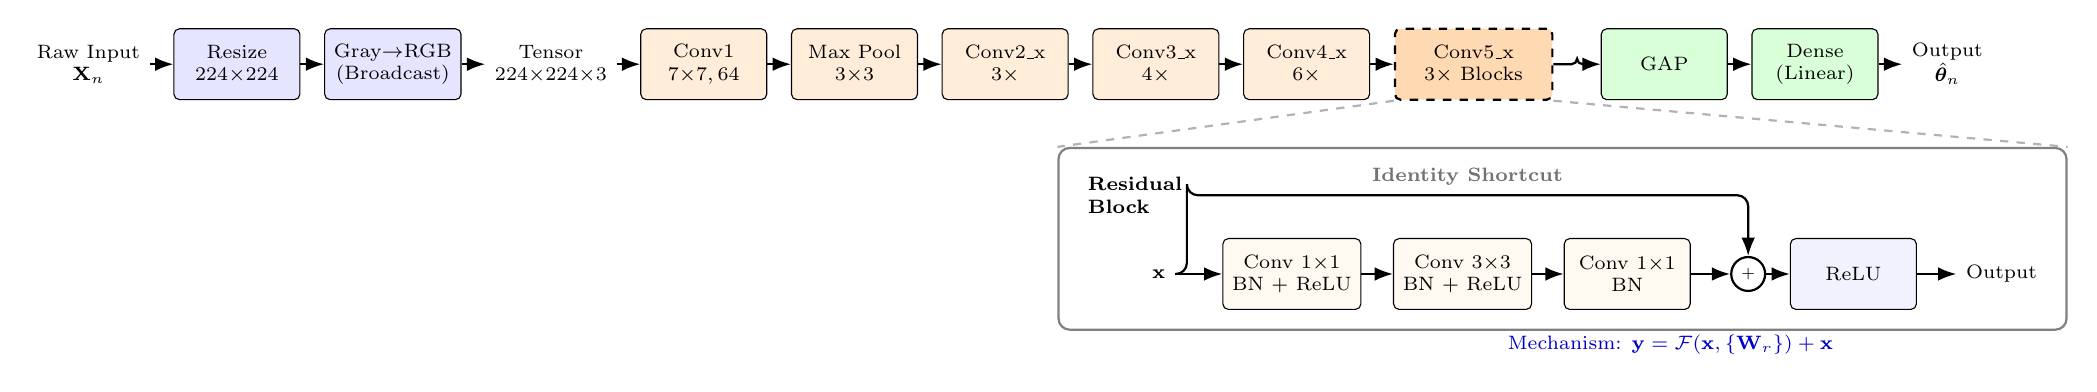
\begin{tikzpicture}[
        % Define styles for the nodes
        base_node/.style={rectangle, draw=black, minimum width=1.6cm, minimum height=0.9cm, align=center, font=\scriptsize, rounded corners=2pt},
        proc_node/.style={base_node, fill=blue!10},
        layer_node/.style={base_node, fill=orange!15},
        special_node/.style={base_node, fill=orange!30, dashed, thick, minimum width=2.0cm},
        head_node/.style={base_node, fill=green!15},
        output_node/.style={rectangle, align=center, font=\scriptsize},
        % Styles for arrows
        arrow/.style={-Latex, thick},
        skip/.style={->, thick, dashed, gray}
    ]

    % =========================================================================
    % MAIN FLOW - INPUT & PREPROCESSING (Horizontal)
    % =========================================================================
    \node (raw_input) [output_node] {Raw Input\\$\mathbf{X}_n$};
    
    \node (resize) [proc_node, right=0.3cm of raw_input] {Resize\\$224{\times}224$};
    \draw [arrow] (raw_input) -- (resize);
    
    \node (rgb_map) [proc_node, right=0.3cm of resize] {Gray$\to$RGB\\(Broadcast)};
    \draw [arrow] (resize) -- (rgb_map);
    
    \node (proc_tensor) [output_node, right=0.3cm of rgb_map] {Tensor\\$224{\times}224{\times}3$};
    \draw [arrow] (rgb_map) -- (proc_tensor);

    % =========================================================================
    % MAIN FLOW - RESNET50 BACKBONE (Horizontal)
    % =========================================================================
    \node (conv1) [layer_node, right=0.3cm of proc_tensor] {Conv1\\$7{\times}7, 64$};
    \draw [arrow] (proc_tensor) -- (conv1);
    
    \node (pool1) [layer_node, right=0.3cm of conv1] {Max Pool\\$3{\times}3$};
    \draw [arrow] (conv1) -- (pool1);

    \node (conv2) [layer_node, right=0.3cm of pool1] {Conv2\_x\\$3\times$};
    \draw [arrow] (pool1) -- (conv2);
    
    \node (conv3) [layer_node, right=0.3cm of conv2] {Conv3\_x\\$4\times$};
    \draw [arrow] (conv2) -- (conv3);
    
    \node (conv4) [layer_node, right=0.3cm of conv3] {Conv4\_x\\$6\times$};
    \draw [arrow] (conv3) -- (conv4);
    
    \node (conv5_detail) [special_node, right=0.3cm of conv4] {Conv5\_x\\$3\times$ Blocks};
    \draw [arrow] (conv4) -- (conv5_detail);

    % Frame for Backbone (Label moved down to sit below the box)
    %\node[draw=orange!80, thick, rounded corners, fit=(conv1) (conv5_detail), inner sep=0.25cm, label={[anchor=north west, orange!80!black, font=\scriptsize\bfseries, yshift=-0.1cm]south west:ResNet50 Backbone}] (backbone_frame) {};

    % =========================================================================
    % MAIN FLOW - REGRESSION HEAD & OUTPUT (Horizontal)
    % =========================================================================
    % Dropped this block down by 2cm using yshift
    \node (gap) [head_node, right=0.6cm of conv5_detail, yshift=0cm] {GAP};
    
    % Routed the arrow cleanly downwards with a right angle
    \draw [arrow, rounded corners=2pt] (conv5_detail.east) -- ++(0.3,0) |- (gap.west);
    
    \node (dense_out) [head_node, right=0.3cm of gap] {Dense\\(Linear)};
    \draw [arrow] (gap) -- (dense_out);
    
    \node (final_output) [output_node, right=0.3cm of dense_out] {Output\\$\hat{\boldsymbol{\theta}}_n$};
    \draw [arrow] (dense_out) -- (final_output);
    
    % Label for Custom Head (Moved down to sit below the box)
    %\node[draw=green!80, thick, rounded corners, fit=(gap) (dense_out), inner sep=0.25cm, label={[anchor=north west, green!80!black, font=\scriptsize\bfseries, yshift=-0.1cm]south west:Regression Head}] (head_frame) {};

    % =========================================================================
    % INSET - BOTTLE NECK RESIDUAL BLOCK (Horizontal)
    % =========================================================================
    % Shift the inset downwards relative to the conv5 block
    \begin{scope}[shift={($(conv5_detail.south)+(-4cm, -2.2cm)$)}]
        
        \node[align=left, font=\scriptsize\bfseries] (inset_title) at (-0.3, 1.0) {Residual\\Block};

        % Inset Nodes (Left to Right)
        \node (in_x) [output_node] at (0, 0) {$\mathbf{x}$};
        
        \node (1x1_reduce) [proc_node, fill=orange!5, right=0.6cm of in_x] {Conv $1{\times}1$\\BN + ReLU};
        \draw [arrow] (in_x) -- (1x1_reduce);
        
        \node (3x3_conv) [proc_node, fill=orange!5, right=0.4cm of 1x1_reduce] {Conv $3{\times}3$\\BN + ReLU};
        \draw [arrow] (1x1_reduce) -- (3x3_conv);
        
        \node (1x1_restore) [proc_node, fill=orange!5, right=0.4cm of 3x3_conv] {Conv $1{\times}1$\\BN};
        \draw [arrow] (3x3_conv) -- (1x1_restore);
        
        \node (plus) [circle, draw, thick, right=0.5cm of 1x1_restore, inner sep=2pt] {\tiny +};
        \draw [arrow] (1x1_restore) -- (plus);
        
        \node (relu_final) [proc_node, fill=blue!5, right=0.3cm of plus] {ReLU};
        \draw [arrow] (plus) -- (relu_final);
        
        \node (out_y) [output_node, right=0.5cm of relu_final] {Output};
        \draw [arrow] (relu_final) -- (out_y);

        % Identity Shortcut (drawn over the top)
        \draw [arrow, rounded corners=4pt] (in_x.east) -- ++(0.15,0) |- ++(0, 1.0) -| node[pos=0.25, above, font=\scriptsize, gray!90!black] {\bfseries Identity Shortcut} (plus.north);
        
        % Math label inside inset
        \node[align=right, font=\scriptsize, blue!80!black] at (6.5, -0.9) 
            {Mechanism: $\mathbf{y} = \mathcal{F}(\mathbf{x}, \{\mathbf{W}_r\}) + \mathbf{x}$};

        % Draw Frame around inset
        \node[draw=gray, thick, fit=(inset_title) (out_y) (relu_final) (in_x), inner sep=0.25cm, rounded corners] (inset_frame) {};
    \end{scope}

    % Dynamic Dashed lines connecting the Backbone to the Inset
    \draw[gray!60, dashed, thick] (conv5_detail.south west) -- (inset_frame.north west);
    \draw[gray!60, dashed, thick] (conv5_detail.south east) -- (inset_frame.north east);

    \end{tikzpicture}
}
\caption{ResNet50 architecture pipeline for Hamiltonian parameter estimation. The pipeline progresses from single-channel input preprocessing through a pre-trained feature extractor. The Residual bottleneck structure used extensively in Conv5\_x. The deepest features are processed by the customized regression head containing a Global Average Pooling (GAP) and a final dense layer with linear activation to output the predicted physical constants.}
\label{fig:resnet_implementation}
\end{figure*}

\item[--] \emph{Densely Connected Convolutional Networks (DenseNet)}~\cite{huang2017densely}: While ResNet adds features via summation, DenseNet concatenates them, maximizing information flow and feature reuse throughout the network. This is particularly advantageous for the Hamiltonian inverse problem, as the delicate energetic competition often manifests in subtle, overlapping spatial frequencies that require dense multi-scale analysis. In a DenseNet block, the feature maps of all preceding layers are used as inputs to the current layer. If $\mathbf{x}_l$ denotes the output of the $l$-th layer, and $H_l(\cdot)$ represents a composite function of batch normalization, ReLU, and convolution, the forward pass is expressed as:

\begin{equation}\label{eq:DenseNet}
\mathbf{x}_l = H_l([\mathbf{x}_0, \mathbf{x}_1, \dots, \mathbf{x}_{l-1}]),
\end{equation}
where $[\dots]$ denotes the concatenation operation. This dense topological structure ensures that the final regression head has direct access to both fine-grained pixel interactions and coarse global structures (see Figure~\ref{fig:densenet_implementation}).

\begin{figure*}[t!]
    \centering
    \resizebox{\linewidth}{!}{
    
    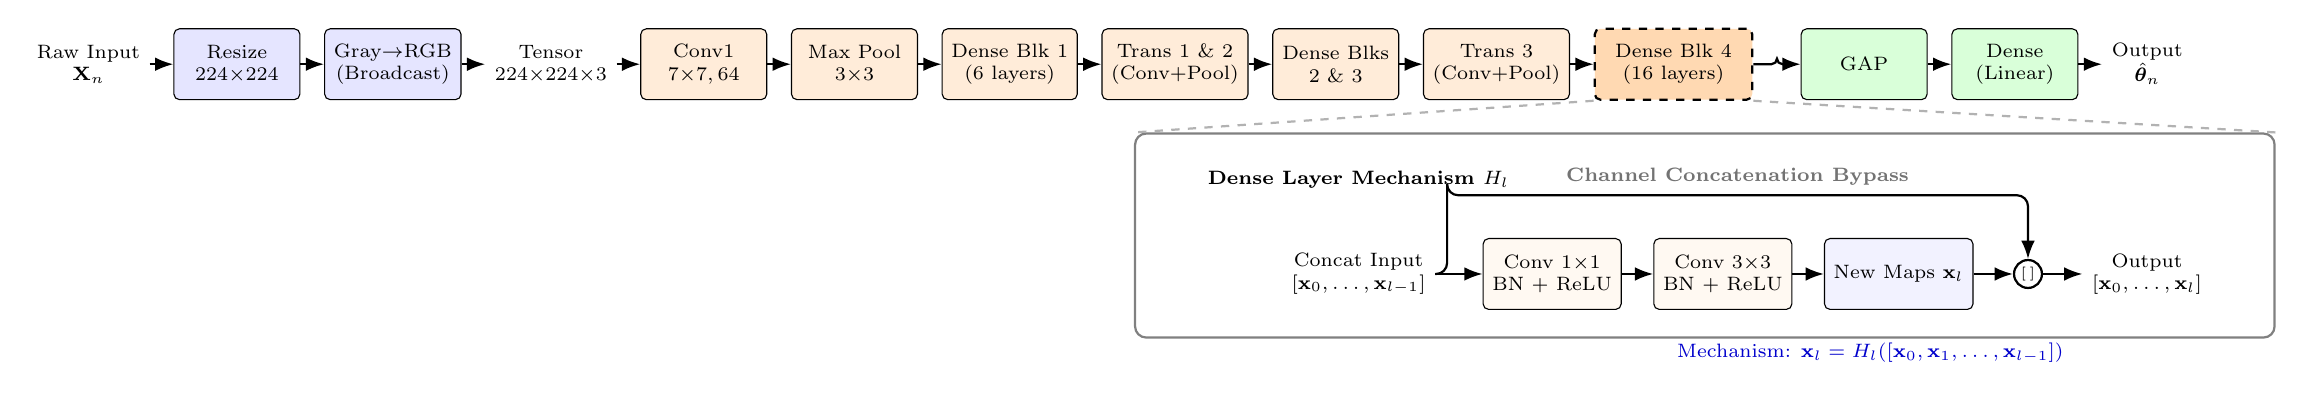
\begin{tikzpicture}[
        % Define styles for the nodes
        base_node/.style={rectangle, draw=black, minimum width=1.6cm, minimum height=0.9cm, align=center, font=\scriptsize, rounded corners=2pt},
        proc_node/.style={base_node, fill=blue!10},
        layer_node/.style={base_node, fill=orange!15},
        special_node/.style={base_node, fill=orange!30, dashed, thick, minimum width=2.0cm},
        head_node/.style={base_node, fill=green!15},
        output_node/.style={rectangle, align=center, font=\scriptsize},
        % Styles for arrows
        arrow/.style={-Latex, thick},
        skip/.style={->, thick, dashed, gray}
    ]

    % =========================================================================
    % MAIN FLOW - INPUT & PREPROCESSING (Horizontal)
    % =========================================================================
    \node (raw_input) [output_node] {Raw Input\\$\mathbf{X}_n$};
    
    \node (resize) [proc_node, right=0.3cm of raw_input] {Resize\\$224{\times}224$};
    \draw [arrow] (raw_input) -- (resize);
    
    \node (rgb_map) [proc_node, right=0.3cm of resize] {Gray$\to$RGB\\(Broadcast)};
    \draw [arrow] (resize) -- (rgb_map);
    
    \node (proc_tensor) [output_node, right=0.3cm of rgb_map] {Tensor\\$224{\times}224{\times}3$};
    \draw [arrow] (rgb_map) -- (proc_tensor);

    % =========================================================================
    % MAIN FLOW - DENSENET121 BACKBONE (Horizontal)
    % =========================================================================
    \node (conv1) [layer_node, right=0.3cm of proc_tensor] {Conv1\\$7{\times}7, 64$};
    \draw [arrow] (proc_tensor) -- (conv1);
    
    \node (pool1) [layer_node, right=0.3cm of conv1] {Max Pool\\$3{\times}3$};
    \draw [arrow] (conv1) -- (pool1);

    \node (db1) [layer_node, right=0.3cm of pool1] {Dense Blk 1\\(6 layers)};
    \draw [arrow] (pool1) -- (db1);
    
    \node (trans1) [layer_node, right=0.3cm of db1] {Trans 1 \& 2\\(Conv+Pool)};
    \draw [arrow] (db1) -- (trans1);
    
    \node (db2_3) [layer_node, right=0.3cm of trans1] {Dense Blks\\2 \& 3};
    \draw [arrow] (trans1) -- (db2_3);
    
    \node (trans3) [layer_node, right=0.3cm of db2_3] {Trans 3\\(Conv+Pool)};
    \draw [arrow] (db2_3) -- (trans3);

    \node (db4_detail) [special_node, right=0.3cm of trans3] {Dense Blk 4\\(16 layers)};
    \draw [arrow] (trans3) -- (db4_detail);

    % Frame for Backbone (Label moved down to sit below the box)
    %\node[draw=orange!80, thick, rounded corners, fit=(conv1) (db4_detail), inner sep=0.25cm, label={[anchor=north west, orange!80!black, font=\scriptsize\bfseries, yshift=-0.1cm]south west:DenseNet121 Backbone}] (backbone_frame) {};

    % =========================================================================
    % MAIN FLOW - REGRESSION HEAD & OUTPUT (Horizontal)
    % =========================================================================
    % Dropped this block down by 2cm using yshift
    \node (gap) [head_node, right=0.6cm of db4_detail, yshift=0cm] {GAP};
    
    % Routed the arrow cleanly downwards with a right angle
    \draw [arrow, rounded corners=2pt] (db4_detail.east) -- ++(0.3,0) |- (gap.west);
    
    \node (dense_out) [head_node, right=0.3cm of gap] {Dense\\(Linear)};
    \draw [arrow] (gap) -- (dense_out);
    
    \node (final_output) [output_node, right=0.3cm of dense_out] {Output\\$\hat{\boldsymbol{\theta}}_n$};
    \draw [arrow] (dense_out) -- (final_output);
    
    % Label for Custom Head (Moved down to sit below the box)
    %\node[draw=green!80, thick, rounded corners, fit=(gap) (dense_out), inner sep=0.25cm, label={[anchor=north west, green!80!black, font=\scriptsize\bfseries, yshift=-0.1cm]south west:Regression Head}] (head_frame) {};

    % =========================================================================
    % INSET - DENSE LAYER CONNECTIVITY (Horizontal)
    % =========================================================================
    % Shift the inset downwards relative to the Dense Block 4
    \begin{scope}[shift={($(db4_detail.south)+(-4cm, -2.2cm)$)}]
        
        \node[align=left, font=\scriptsize\bfseries] (inset_title) at (0, 1.2) {Dense Layer Mechanism $H_l$};

        % Inset Nodes (Left to Right)
        \node (in_concat) [output_node] at (0, 0) {Concat Input\\$[\mathbf{x}_0, \dots, \mathbf{x}_{l-1}]$};
        
        \node (1x1_conv) [proc_node, fill=orange!5, right=0.6cm of in_concat] {Conv $1{\times}1$\\BN + ReLU};
        \draw [arrow] (in_concat) -- (1x1_conv);
        
        \node (3x3_conv) [proc_node, fill=orange!5, right=0.4cm of 1x1_conv] {Conv $3{\times}3$\\BN + ReLU};
        \draw [arrow] (1x1_conv) -- (3x3_conv);
        
        \node (new_feat) [proc_node, fill=blue!5, right=0.4cm of 3x3_conv] {New Maps $\mathbf{x}_l$};
        \draw [arrow] (3x3_conv) -- (new_feat);

        \node (concat_out) [circle, draw, thick, right=0.5cm of new_feat, inner sep=1pt] {\tiny $[\,]$};
        \draw [arrow] (new_feat) -- (concat_out);
        
        \node (out_y) [output_node, right=0.5cm of concat_out] {Output\\$[\mathbf{x}_0, \dots, \mathbf{x}_l]$};
        \draw [arrow] (concat_out) -- (out_y);

        % Dense Connectivity Shortcut (drawn over the top)
        \draw [arrow, rounded corners=4pt] (in_concat.east) -- ++(0.15,0) |- ++(0, 1.0) -| node[pos=0.25, above, font=\scriptsize, gray!90!black] {\bfseries Channel Concatenation Bypass} (concat_out.north);
        
        % Math label inside inset
        \node[align=right, font=\scriptsize, blue!80!black] at (6.5, -1.0) 
            {Mechanism: $\mathbf{x}_l = H_l([\mathbf{x}_0, \mathbf{x}_1, \dots, \mathbf{x}_{l-1}])$};

        % Draw Frame around inset
        \node[draw=gray, thick, fit=(inset_title) (out_y) (new_feat) (in_concat), inner sep=0.35cm, inner xsep=0.8cm, rounded corners] (inset_frame) {};
    \end{scope}

    % Dynamic Dashed lines connecting the Backbone to the Inset
    \draw[gray!60, dashed, thick] (db4_detail.south west) -- (inset_frame.north west);
    \draw[gray!60, dashed, thick] (db4_detail.south east) -- (inset_frame.north east);

    \end{tikzpicture}
}
\caption{DenseNet121 architecture pipeline for Hamiltonian parameter estimation. The pipeline progresses left-to-right, processing single-channel inputs through the feature extractor composed of Dense Blocks and Transition layers. A detailed horizontal view illustrates the dense connectivity mechanism where feature maps from all preceding layers are concatenated before convolution. The final aggregated features are mapped to physical constants via the customized regression head.}
\label{fig:densenet_implementation}
\end{figure*}


\item[--] \emph{Xception (Extreme Inception)}~\cite{chollet2017xception}: This architecture operates on the hypothesis that cross-channel correlations and spatial correlations in feature maps can be entirely decoupled. It replaces standard Inception modules with depthwise separable convolutions, drastically reducing computational overhead while enhancing representational efficiency. A depthwise separable convolution splits the standard convolution into two distinct steps. First, a depthwise convolution applies a single spatial filter to each input channel independently. Second, a pointwise convolution ($1 \times 1$ convolution) projects the output of the depthwise step onto a new channel space to capture cross-channel correlations. If $\mathbf{X} \in \mathbb{R}^{\breve{H} \times \breve{W} \times \breve{C}}$ is the input tensor, the operation is formally approximated as:

\begin{equation}\label{eq:Xception}
\text{Conv}_{\text{sep}}(\mathbf{X}) = \text{Conv}_{\text{pointwise}}(\text{Conv}_{\text{depthwise}}(\mathbf{X})).
\end{equation}

For nanoscale magnetism, this extreme decoupling allows the network to efficiently isolate specific topological frequency patterns (depthwise) before correlating them to the complex parameter space $\boldsymbol{\theta}_n$ (see Figure~\ref{fig:xception_implementation}).

\begin{figure*}[t!]
    \centering
    \resizebox{\linewidth}{!}{
    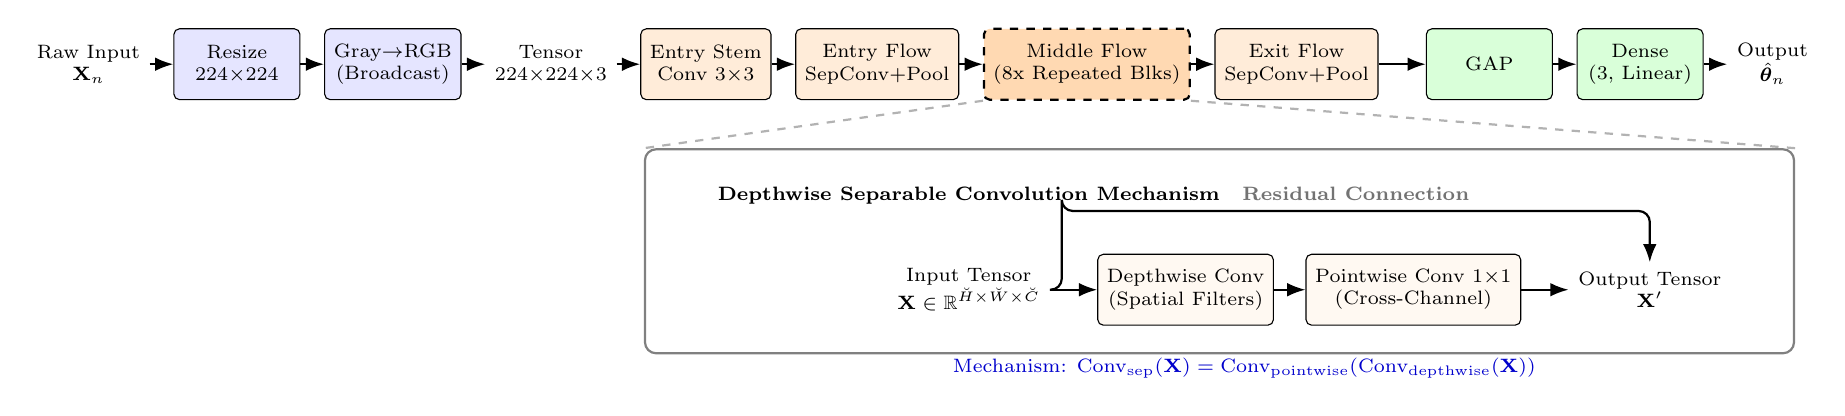
\begin{tikzpicture}[
    % Define styles for the nodes
    base_node/.style={rectangle, draw=black, minimum width=1.6cm, minimum height=0.9cm, align=center, font=\scriptsize, rounded corners=2pt},
    proc_node/.style={base_node, fill=blue!10},
    layer_node/.style={base_node, fill=orange!15},
    special_node/.style={base_node, fill=orange!30, dashed, thick, minimum width=2.0cm},
    head_node/.style={base_node, fill=green!15},
    output_node/.style={rectangle, align=center, font=\scriptsize},
    % Styles for arrows
    arrow/.style={-Latex, thick},
    skip/.style={->, thick, dashed, gray}
]

    % =========================================================================
    % MAIN FLOW - INPUT & PREPROCESSING (Horizontal)
    % =========================================================================
    \node (raw_input) [output_node] {Raw Input\\$\mathbf{X}_n$};
    
    \node (resize) [proc_node, right=0.3cm of raw_input] {Resize\\$224{\times}224$};
    \draw [arrow] (raw_input) -- (resize);
    
    \node (rgb_map) [proc_node, right=0.3cm of resize] {Gray$\to$RGB\\(Broadcast)};
    \draw [arrow] (resize) -- (rgb_map);
    
    \node (proc_tensor) [output_node, right=0.3cm of rgb_map] {Tensor\\$224{\times}224{\times}3$};
    \draw [arrow] (rgb_map) -- (proc_tensor);

    % =========================================================================
    % MAIN FLOW - XCEPTION BACKBONE (Horizontal)
    % =========================================================================
    \node (entry_stem) [layer_node, right=0.3cm of proc_tensor] {Entry Stem\\Conv $3{\times}3$};
    \draw [arrow] (proc_tensor) -- (entry_stem);
    
    \node (entry_blocks) [layer_node, right=0.3cm of entry_stem] {Entry Flow\\SepConv+Pool};
    \draw [arrow] (entry_stem) -- (entry_blocks);

    % Highlight the Middle flow as the special node linking to the inset
    \node (mid_flow) [special_node, right=0.3cm of entry_blocks] {Middle Flow\\(8x Repeated Blks)};
    \draw [arrow] (entry_blocks) -- (mid_flow);
    
    \node (exit_flow) [layer_node, right=0.3cm of mid_flow] {Exit Flow\\SepConv+Pool};
    \draw [arrow] (mid_flow) -- (exit_flow);

    % =========================================================================
    % MAIN FLOW - REGRESSION HEAD & OUTPUT (Horizontal)
    % =========================================================================
    \node (gap) [head_node, right=0.6cm of exit_flow] {GAP};
    \draw [arrow] (exit_flow) -- (gap);
    
    \node (dense_out) [head_node, right=0.3cm of gap] {Dense\\(3, Linear)};
    \draw [arrow] (gap) -- (dense_out);
    
    \node (final_output) [output_node, right=0.3cm of dense_out] {Output\\$\hat{\boldsymbol{\theta}}_n$};
    \draw [arrow] (dense_out) -- (final_output);

    % =========================================================================
    % INSET - DEPTHWISE SEPARABLE CONVOLUTION (Horizontal)
    % =========================================================================
    % Shift the inset downwards relative to the Middle Flow node
    \begin{scope}[shift={($(mid_flow.south)+(-1.5cm, -2.4cm)$)}]
        
        \node[align=left, font=\scriptsize\bfseries] (inset_title) at (0, 1.2) {Depthwise Separable Convolution Mechanism};

        % Inset Nodes (Left to Right)
        \node (in_tensor) [output_node] at (0, 0) {Input Tensor\\$\mathbf{X} \in \mathbb{R}^{\breve{H} \times \breve{W} \times \breve{C}}$};
        
        \node (dw_conv) [proc_node, fill=orange!5, right=0.6cm of in_tensor] {Depthwise Conv\\(Spatial Filters)};
        \draw [arrow] (in_tensor) -- (dw_conv);
        
        \node (pw_conv) [proc_node, fill=orange!5, right=0.4cm of dw_conv] {Pointwise Conv $1{\times}1$\\(Cross-Channel)};
        \draw [arrow] (dw_conv) -- (pw_conv);
        
        \node (out_tensor) [output_node, right=0.6cm of pw_conv] {Output Tensor\\$\mathbf{X}'$};
        \draw [arrow] (pw_conv) -- (out_tensor);

        % Residual Connection Shortcut (drawn over the top)
        \draw [arrow, rounded corners=4pt] (in_tensor.east) -- ++(0.15,0) |- ++(0, 1.0) -| node[pos=0.25, above, font=\scriptsize, gray!90!black] {\bfseries Residual Connection} (out_tensor.north);
        
        % Math label inside inset mapping to the paper's equation
        \node[align=center, font=\scriptsize, blue!80!black] at (3.5, -1.0) 
            {Mechanism: $\text{Conv}_{\text{sep}}(\mathbf{X}) = \text{Conv}_{\text{pointwise}}(\text{Conv}_{\text{depthwise}}(\mathbf{X}))$};

        % Draw Frame around inset
        \node[draw=gray, thick, fit=(inset_title) (out_tensor) (dw_conv) (in_tensor) (pw_conv), inner sep=0.35cm, inner xsep=0.8cm, rounded corners] (inset_frame) {};
    \end{scope}

    % Dynamic Dashed lines connecting the Backbone to the Inset
    \draw[gray!60, dashed, thick] (mid_flow.south west) -- (inset_frame.north west);
    \draw[gray!60, dashed, thick] (mid_flow.south east) -- (inset_frame.north east);

\end{tikzpicture}}
\caption{Xception architecture pipeline for Hamiltonian parameter estimation. The feature extractor composed of Entry, Middle, and Exit flows. A detailed horizontal view illustrates the depthwise separable convolution mechanism where spatial feature extraction (depthwise) and cross-channel correlations (pointwise) are entirely decoupled. The final aggregated features are mapped to physical constants.}\label{fig:xception_implementation}
\end{figure*}



\item[--] \emph{Visual Transformer (ViT)}~\cite{dosovitskiy2020image}: Unlike Convolutional Neural Networks, which enforce a strict local inductive bias, the Vision Transformer processes the 2D spatial magnetization field $\mathbf{X}_n$ as a sequence of flattened, non-overlapping 2D patches. This allows the model to capture long-range, global dependencies across the nanodot instantly, which is critical for understanding macro-scale topological stability dictated by the Zeeman field or global anisotropy. The input image is divided into $N_p$ patches, which are linearly projected into a sequence of $D$-dimensional embeddings. The core mechanism is the Multi-Head Self-Attention (MSA), which computes attention scores to weigh the importance of different patches relative to one another. For a given set of queries $Q$, keys $K$, and values $V$ derived from the patch embeddings, the scaled dot-product attention is defined as:

\begin{equation}\label{eq:ViT}
\text{Attention}(Q, K, V) = \text{softmax}\left(\frac{QK^\top}{\sqrt{d_k}}\right)V,
\end{equation}
where $d_k$ is the scaling factor (the dimension of the keys). By employing MSA, the ViT can explicitly correlate a localized structural defect on one edge of the nanodot with a compensatory chiral boundary on the opposite edge, mapping these distant correlations directly to the global DMI or symmetric exchange strengths.

\begin{figure*}[t!]
    \centering
    \resizebox{\linewidth}{!}{
    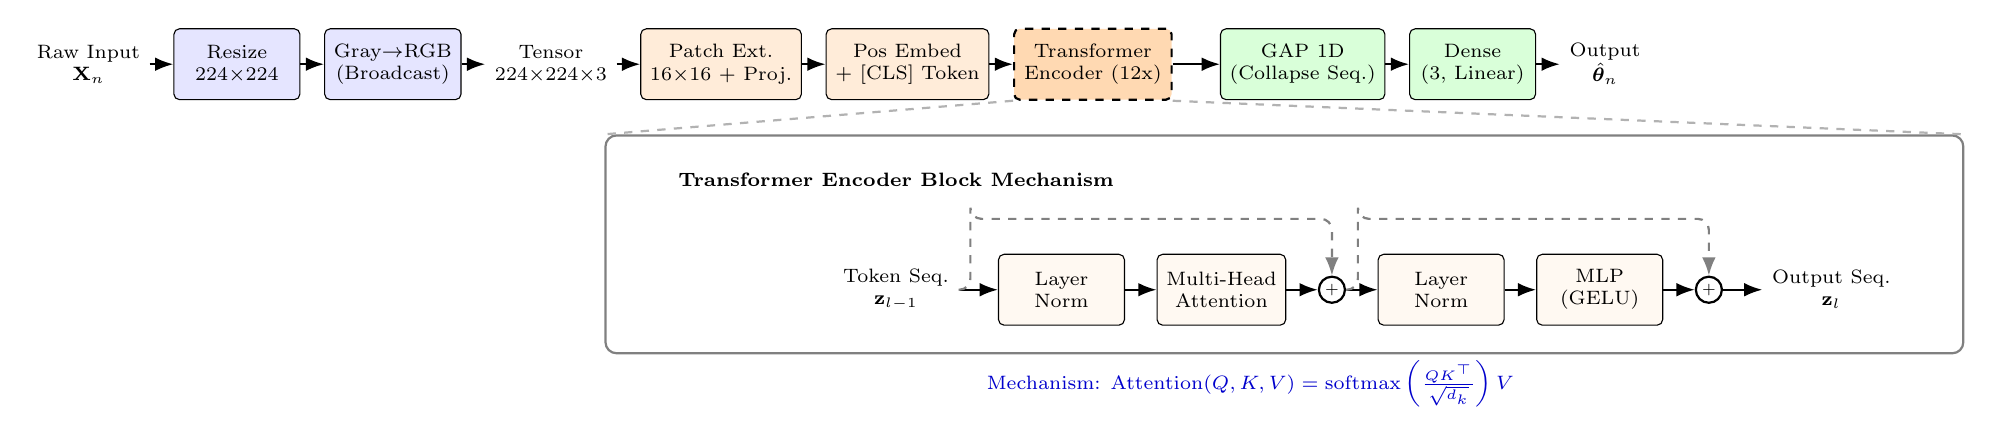
\begin{tikzpicture}[
    % Define styles for the nodes
    base_node/.style={rectangle, draw=black, minimum width=1.6cm, minimum height=0.9cm, align=center, font=\scriptsize, rounded corners=2pt},
    proc_node/.style={base_node, fill=blue!10},
    layer_node/.style={base_node, fill=orange!15},
    special_node/.style={base_node, fill=orange!30, dashed, thick, minimum width=2.0cm},
    head_node/.style={base_node, fill=green!15},
    output_node/.style={rectangle, align=center, font=\scriptsize},
    add_node/.style={circle, draw, thick, inner sep=1pt, font=\tiny},
    % Styles for arrows
    arrow/.style={-Latex, thick},
    skip/.style={-Latex, thick, dashed, gray}
]

    % =========================================================================
    % MAIN FLOW - INPUT & PREPROCESSING (Horizontal)
    % =========================================================================
    \node (raw_input) [output_node] {Raw Input\\$\mathbf{X}_n$};
    
    \node (resize) [proc_node, right=0.3cm of raw_input] {Resize\\$224{\times}224$};
    \draw [arrow] (raw_input) -- (resize);
    
    \node (rgb_map) [proc_node, right=0.3cm of resize] {Gray$\to$RGB\\(Broadcast)};
    \draw [arrow] (resize) -- (rgb_map);
    
    \node (proc_tensor) [output_node, right=0.3cm of rgb_map] {Tensor\\$224{\times}224{\times}3$};
    \draw [arrow] (rgb_map) -- (proc_tensor);

    % =========================================================================
    % MAIN FLOW - VISION TRANSFORMER BACKBONE (Horizontal)
    % =========================================================================
    \node (patching) [layer_node, right=0.3cm of proc_tensor] {Patch Ext.\\$16{\times}16$ + Proj.};
    \draw [arrow] (proc_tensor) -- (patching);
    
    \node (pos_embed) [layer_node, right=0.3cm of patching] {Pos Embed\\+ [CLS] Token};
    \draw [arrow] (patching) -- (pos_embed);

    % Highlight the Transformer Blocks as the special node linking to the inset
    \node (transformer) [special_node, right=0.3cm of pos_embed] {Transformer\\Encoder (12x)};
    \draw [arrow] (pos_embed) -- (transformer);

    % =========================================================================
    % MAIN FLOW - REGRESSION HEAD & OUTPUT (Horizontal)
    % =========================================================================
    % Using GAP1D as per the specific code implementation
    \node (gap1d) [head_node, right=0.6cm of transformer] {GAP 1D\\(Collapse Seq.)};
    \draw [arrow] (transformer) -- (gap1d);
    
    \node (dense_out) [head_node, right=0.3cm of gap1d] {Dense\\(3, Linear)};
    \draw [arrow] (gap1d) -- (dense_out);
    
    \node (final_output) [output_node, right=0.3cm of dense_out] {Output\\$\hat{\boldsymbol{\theta}}_n$};
    \draw [arrow] (dense_out) -- (final_output);

    % =========================================================================
    % INSET - TRANSFORMER ENCODER BLOCK (Horizontal)
    % =========================================================================
    % Shift the inset downwards relative to the Transformer node
    \begin{scope}[shift={($(transformer.south)+(-2.5cm, -2.4cm)$)}]
        
        \node[align=left, font=\scriptsize\bfseries] (inset_title) at (0, 1.4) {Transformer Encoder Block Mechanism};

        % Inset Nodes (Left to Right)
        \node (in_seq) [output_node] at (0, 0) {Token Seq.\\$\mathbf{z}_{l-1}$};
        
        \node (norm1) [proc_node, fill=orange!5, right=0.5cm of in_seq] {Layer\\Norm};
        \draw [arrow] (in_seq) -- (norm1);
        
        \node (msa) [proc_node, fill=orange!5, right=0.4cm of norm1] {Multi-Head\\Attention};
        \draw [arrow] (norm1) -- (msa);
        
        \node (add1) [add_node, right=0.4cm of msa] {$+$};
        \draw [arrow] (msa) -- (add1);
        
        \node (norm2) [proc_node, fill=orange!5, right=0.4cm of add1] {Layer\\Norm};
        \draw [arrow] (add1) -- (norm2);
        
        \node (mlp) [proc_node, fill=orange!5, right=0.4cm of norm2] {MLP\\(GELU)};
        \draw [arrow] (norm2) -- (mlp);
        
        \node (add2) [add_node, right=0.4cm of mlp] {$+$};
        \draw [arrow] (mlp) -- (add2);
        
        \node (out_seq) [output_node, right=0.5cm of add2] {Output Seq.\\$\mathbf{z}_l$};
        \draw [arrow] (add2) -- (out_seq);

        % Residual Connections (drawn over the top)
        \draw [skip, rounded corners=4pt] (in_seq.east) -- ++(0.15,0) |- ++(0, 0.9) -| (add1.north);
        \draw [skip, rounded corners=4pt] (add1.east) -- ++(0.15,0) |- ++(0, 0.9) -| (add2.north);
        
        % Math label inside inset mapping to the paper's equation
        \node[align=center, font=\scriptsize, blue!80!black] at (4.5, -1.2) 
            {Mechanism: $\text{Attention}(Q, K, V) = \text{softmax}\left(\frac{QK^\top}{\sqrt{d_k}}\right)V$};

        % Draw Frame around inset
        \node[draw=gray, thick, fit=(inset_title) (out_seq) (msa) (mlp) (in_seq), inner sep=0.35cm, inner xsep=0.8cm, rounded corners] (inset_frame) {};
    \end{scope}

    % Dynamic Dashed lines connecting the Backbone to the Inset
    \draw[gray!60, dashed, thick] (transformer.south west) -- (inset_frame.north west);
    \draw[gray!60, dashed, thick] (transformer.south east) -- (inset_frame.north east);

\end{tikzpicture}}
\caption{ViT architecture pipeline for Hamiltonian parameter estimation. The pipeline progresses left-to-right, processing single-channel inputs through patch extraction, linear projection, and a sequential backbone of Transformer Encoder blocks. The core Transformer block mechanism, highlighting the MSA that explicitly models long-range spatial dependencies across the magnetic nanodot. The final sequence of high-level token representations is aggregated via 1D GAP and mapped to the physical constants through the customized regression head.}
\label{fig:vit_implementation}
\end{figure*}


To optimize the parameter set $\hat{\Theta}$ in Equation~\ref{eq:LossFunction} across all evaluated architectures, the models are trained utilizing the MSE as the explicit continuous loss function $\mathcal{L}$. The optimization process is executed using the Adam optimizer, relying on backpropagation and automatic differentiation to efficiently compute the network gradients~\cite{murakami2022inverse}. By iteratively updating the model weights based on these computed gradients, the training pipeline systematically minimizes the structural and energetic discrepancies between the predicted outputs and the true Hamiltonian constants, ensuring robust convergence in estimating the underlying physical parameters.

\end{itemize}

\subsection{Spatial Interpretability via RAMs}\label{sec:RAMs}

Interpretability methods based on activation mapping have become a foundational approach for understanding the decision-making processes of deep neural networks. By identifying the spatial regions within an input that most significantly influence a model's prediction, these methods project opaque latent representations back into a human-interpretable domain. Among these, Gradient-weighted Class Activation Mapping (Grad-CAM) and its variants have been extensively utilized in computer vision to generate class-specific saliency maps~\cite{vinogradova2020gradcam}. 

In standard classification paradigms, given an input image $\mathbf{X}$ and a discrete target class score $y^c$, activation maps are computed by extracting the gradients of $y^c$ with respect to the $k$-th feature map $\mathbf{A}^k \in \mathbb{R}^{H' \times W'}$ of a terminal convolutional layer (where $H'$ and $W'$ denote the spatial dimensions of the feature map). The spatial importance weights are derived by globally pooling these gradients, and the final map is a ReLU-activated linear combination of the feature maps~\cite{zhang2024gradcam}. While highly effective for discrete semantic categorization, this standard formulation structurally fails in continuous regression tasks. The absence of a discrete target class removes the natural selection mechanism required to isolate the output dimension driving the interpretability process. Furthermore, directly computing gradients with respect to a prediction $\hat{\boldsymbol{\theta}}$ introduces severe gradient instability; minute fluctuations in the scalar output can yield drastically different spatial attributions, failing to provide the physical consistency required for analyzing complex Hamiltonian parameters~\cite{makke2024symbolic}.

\subsubsection{RAMs for CNN-based Approaches}\label{sec:CNN_RAMs}

To overcome the fundamental limitations of discrete activation methods in highly degenerate physical systems, we introduce RAMs, a novel formulation explicitly tailored to bridge continuous parameter estimation with spatial topologies. Given an input magnetic domain visualization $\mathbf{X}$ and the optimized regression model $f_{\hat{\Theta}} : \mathbb{R}^{\breve{H} \times \breve{W}} \rightarrow \mathbb{R}^{\breve{P}}$, the network predicts a vector of physical constants $\hat{\boldsymbol{\theta}} = f_{\hat{\Theta}}(\mathbf{X})$. Let $\hat{\theta}_p \in \hat{\boldsymbol{\theta}}$ denote the continuous prediction for the $p$-th target Hamiltonian parameter (e.g., the DMI strength $\tilde{D}$ or symmetric exchange $\tilde{J}$), and let $\theta_p \in \boldsymbol{\theta}$ represents its corresponding ground truth. Instead of utilizing a raw predicted scalar, we formulate a scale-invariant, error-based activation objective $\mathcal{O}_p$. To prevent the mathematical discontinuities and negative objective bounds inherent to absolute error formulations ($1 - |\theta_p - \hat{\theta}_p|$), we utilize a normalized Gaussian decay function:

\begin{equation}\label{eq:RAM_Objective}
\mathcal{O}_p = \exp\left(-\gamma_p \left(\theta_p - \hat{\theta}_p\right)^2\right),
\end{equation}
where $\gamma_p>0$ is a hyperparameter-specific precision factor determining the strictness of the error decay. This objective smoothly bounds the activation target strictly within $(0, 1]$, promoting maximum gradient response precisely when the network's prediction asymptotically approaches the true thermodynamic value, thereby isolating the topological features that positively contribute to accurate regression.

The spatial importance weights $\alpha_k^{(p)}$ for each continuous feature map $\mathbf{A}^k$ are subsequently computed by globally averaging the gradients of the error objective $\mathcal{O}_p$ with respect to the local spatial activations $\mathbf{A}_{ij}^k$:

\begin{equation}\label{eq:RAM_Weights}
\alpha_k^{(p)} = \frac{1}{H' W'} \sum_{i=1}^{H'} \sum_{j=1}^{W'} \frac{\partial \mathcal{O}_p}{\partial \mathbf{A}_{ij}^k}.
\end{equation}

These weights strictly quantify the importance of the $k$-th latent spatial feature in successfully minimizing the prediction error for the target physical parameter $\theta_p$. The resulting RAM is then formulated as:

\begin{equation}\label{eq:RAM_Formulation}
\mathbf{\mathcal{R}}_{\text{RAM}}^{(p)} = \text{ReLU} \left( \sum_k \alpha_k^{(p)} \mathbf{A}^k \right).
\end{equation}

The application of the ReLU activation ensures that only spatial features exerting a positive, stabilizing influence on the estimation of the target parameter are preserved. Finally, $\mathcal{R}_{\text{RAM}}^{(p)}$ is spatially upsampled to the original input resolution $\breve{H} \times \breve{W}$ and normalized to the interval $[0,1]$. Then, by mapping the continuous error gradients back to the input spatial magnetization field $\mathbf{X}$, RAMs allow for the direct visual and quantitative identification of the specific emergent textures that the network utilizes to deduce the underlying energetic balances. The complete workflow for this localized spatial interpretability is illustrated in Figure~\ref{fig:rams_pipeline}.


%RAMs
\begin{figure*}[t!]
  \centering
  \vspace{0.3cm}
  \resizebox{0.7\linewidth}{!}{
      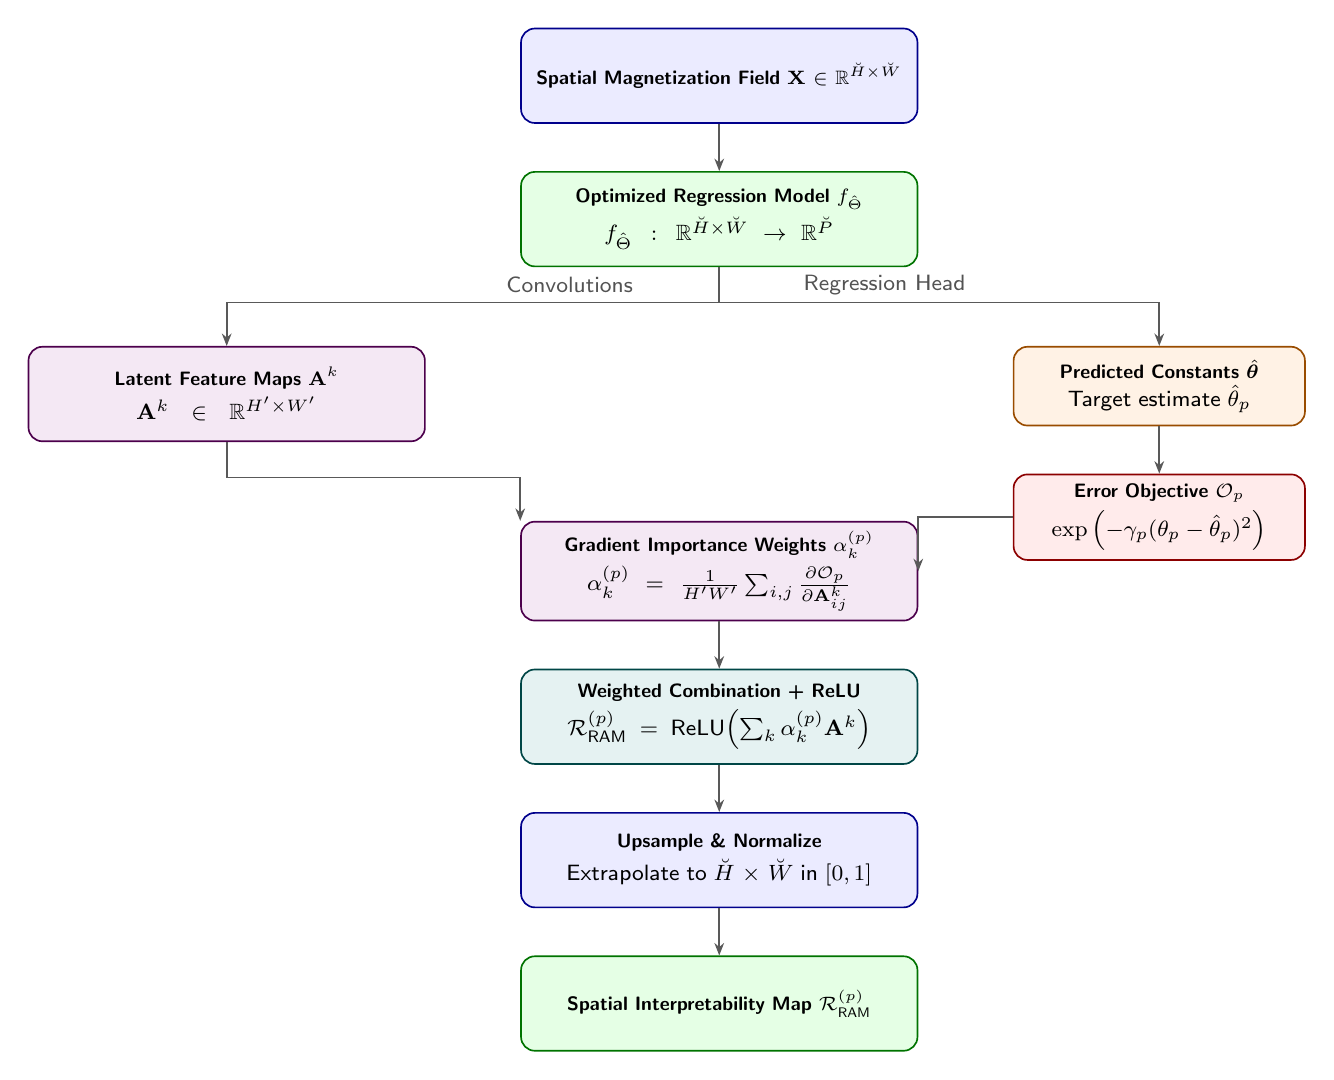
\begin{tikzpicture}[
      node distance = 0.6cm and 1.0cm,
      every node/.style = {font=\scriptsize\sffamily},
      blk/.style = {
        rectangle, rounded corners=5pt,
        minimum width=5.0cm, minimum height=1.2cm,
        text centered, text width=4.8cm,
        draw, line width=0.6pt
      },
      blkN/.style = {
        rectangle, rounded corners=5pt,
        minimum width=3.7cm, minimum height=1.0cm,
        text centered, text width=2.8cm,
        draw, line width=0.6pt
      },
      cinput/.style  = {blk,  fill=blue!8,    draw=blue!55!black},
      cmodel/.style  = {blk,  fill=green!10,  draw=green!45!black},
      cfeat/.style   = {blk,  fill=violet!9,  draw=violet!60!black},
      cpred/.style   = {blkN, fill=orange!10, draw=orange!60!black},
      cerror/.style  = {blkN, fill=red!8,     draw=red!55!black},
      cgrad/.style   = {blk,  fill=violet!9,  draw=violet!60!black},
      crelu/.style   = {blk,  fill=teal!10,   draw=teal!55!black},
      cnorm/.style   = {blk,  fill=blue!8,    draw=blue!55!black},
      cout/.style    = {blk,  fill=green!10,  draw=green!45!black},
      arr/.style = {-{Stealth[length=4.5pt, width=3.5pt]},
                    line width=0.6pt, gray!70!black},
    ]
    \node[cinput] (input)
      {\textbf{Spatial Magnetization Field} $\mathbf{X} \in \mathbb{R}^{\breve{H} \times \breve{W}}$};
    \node[cmodel, below=of input] (model)
      {\textbf{Optimized Regression Model} $f_{\hat{\Theta}}$\\[2pt]
       {\footnotesize $f_{\hat{\Theta}}:\mathbb{R}^{\breve{H} \times \breve{W}}\!\to\!\mathbb{R}^{\breve{P}}$}};
    \node[cfeat, below left=1.0cm and 1.2cm of model] (feat)
      {\textbf{Latent Feature Maps} $\mathbf{A}^{k}$\\[2pt]
       {\footnotesize $\mathbf{A}^{k}\in\mathbb{R}^{H' \times W'}$}};
    \node[cpred, below right=1.0cm and 1.2cm of model] (pred)
      {\textbf{Predicted Constants} $\hat{\boldsymbol{\theta}}$\\[2pt]
       {\footnotesize Target estimate $\hat{\theta}_{p}$}};
    \node[cerror, below=0.6cm of pred] (error)
      {\textbf{Error Objective} $\mathcal{O}_{p}$\\[2pt]
       {\footnotesize $\exp\left(-\gamma_p (\theta_p - \hat{\theta}_p)^2\right)$}};
    \node[cgrad, below right=1.0cm and 1.2cm of feat] (grad)
      {\textbf{Gradient Importance Weights} $\alpha_{k}^{(p)}$\\[2pt]
       {\footnotesize $\alpha_{k}^{(p)}=\frac{1}{H' W'}
         \sum_{i,j}\frac{\partial\mathcal{O}_{p}}
         {\partial \mathbf{A}^{k}_{ij}}$}};
    \node[crelu, below=0.6cm of grad] (relu)
      {\textbf{Weighted Combination + ReLU}\\[2pt]
       {\footnotesize $\mathcal{R}_{\text{RAM}}^{(p)}=
         \text{ReLU}\!\left(\sum_{k}
         \alpha_{k}^{(p)} \mathbf{A}^{k}\right)$}};
    \node[cnorm, below=0.6cm of relu] (norm)
      {\textbf{Upsample \& Normalize}\\[2pt]
       {\footnotesize Extrapolate to $\breve{H} \times \breve{W}$ in $[0,1]$}};
    \node[cout, below=0.6cm of norm] (out)
      {\textbf{Spatial Interpretability Map} $\mathcal{R}_{\text{RAM}}^{(p)}$};
    \draw[arr] (input) -- (model);
    \draw[arr] (model.south) -- ++(0,-0.45) -| (feat.north);
    \node[font=\footnotesize\sffamily, gray!65!black]
      at ($(model.south)+(-1.9,-0.22)$) {Convolutions};
    \draw[arr] (model.south) -- ++(0,-0.45) -| (pred.north);
    \node[font=\footnotesize\sffamily, gray!65!black]
      at ($(model.south)+(2.1,-0.22)$) {Regression Head};
    \draw[arr] (pred) -- (error);
    \draw[arr] (feat.south) -- ++(0,-0.45) -| (grad.north west);
    \draw[arr] (error.west) -- ++(0,0) -| (grad.east);
    \draw[arr] (grad) -- (relu);
    \draw[arr] (relu) -- (norm);
    \draw[arr] (norm) -- (out);
    \end{tikzpicture}
  }
  \caption{RAMs extraction pipeline. Latent feature maps and continuous predictions from the network backbone are explicitly coupled via an error-decay objective. Gradient-based importance weights combine these features to produce a normalized, physically traceable spatial saliency map for the target Hamiltonian parameter $\theta_{p}$.}
  \label{fig:rams_pipeline}
\end{figure*}


\subsubsection{RAMs for ViT-based Approaches}\label{sec:ViT_RAMs}
%ViT RAMs
While our standard RAMs formulation seamlessly integrates with CNNs by exploiting their innate spatial hierarchies, extending this interpretability metric to the Vision Transformers requires mapping sequence-based latent representations back to the two-dimensional physical domain. Unlike CNNs, which preserve spatial locality through sliding convolutional filters, the ViT processes the input spatial magnetization field $\mathbf{X}$ as a flattened sequence of $N_r$ non-overlapping patches, outputting a discrete sequence of latent embeddings. To evaluate ViT-based architectures within the exact same RAMs framework, we introduce a token-reshaping mechanism that bridges the one-dimensional transformer latent space with the two-dimensional topological geometry. Let the output of the terminal Transformer encoder block be denoted as $\mathbf{Z} \in \mathbb{R}^{(N_r + 1) \times D}$, where $D$ is the embedding dimension and the extra token corresponds to the global aggregation token (e.g., the \texttt{[CLS]} token) utilized by the regression head to predict the Hamiltonian parameters $\hat{\mathbf{y}}$. By isolating the $N_r$ spatial tokens, we obtain the localized sequence $\mathbf{Z}_s \in \mathbb{R}^{N_r \times D}$. Because each sequence token explicitly corresponds to a fixed physical patch of the original nanodot domain, $\mathbf{Z}_s$ can be folded back into a 2D spatial grid. Assuming square patches, the sequence is reshaped into a pseudo-feature map:

\begin{equation}\label{eq:ViT_Reshape}
\mathbf{A}_{\text{ViT}} = \text{Reshape}(\mathbf{Z}_s) \in \mathbb{R}^{\sqrt{N_r} \times \sqrt{N_r} \times D}.
\end{equation}

Once projected into this tensor format, $\mathbf{A}_{\text{ViT}}$ functions structurally identically to the terminal convolutional feature map $\mathbf{A}$ utilized in the CNN baseline. The $k$-th slice of the embedding dimension ($k \in \{1, \dots, D\}$) forms the latent spatial map $\mathbf{A}_{\text{ViT}}^k \in \mathbb{R}^{\sqrt{N_r} \times \sqrt{N_r}}$. We then apply the identical scale-invariant, error-based activation objective $\mathcal{O}_p$ defined in Equation~\ref{eq:RAM_Objective}. The spatial importance weights for the ViT embeddings are computed by globally averaging the gradients of this objective with respect to the reshaped spatial tokens:

\begin{equation}\label{eq:ViT_Weights}
\alpha_k^{(p)} = \frac{1}{N_r} \sum_{i=1}^{\sqrt{N_r}} \sum_{j=1}^{\sqrt{N_r}} \frac{\partial \mathcal{O}_p}{\partial (\mathbf{A}_{\text{ViT}})_{ij}^k}.
\end{equation}

RAMs for the ViT are constructed via the ReLU-activated linear combination of these reshaped embedding slices, precisely mirroring Equation~\ref{eq:RAM_Formulation}, before being upsampled to the original input resolution $\breve{H} \times \breve{W}$. This extension guarantees an architecture-agnostic evaluation of interpretability, ensuring that the isolated degenerate textures driving the model's predictions can be fairly compared across fundamentally disparate deep learning architectures.

\subsubsection{Normalized RAMs for Layer-Wise and Target-Specific Analysis}\label{sec:Nor_RAMs}

To rigorously compare the spatial activations across different Hamiltonian parameters and network depths, it is imperative to compute the RAMs utilizing strictly normalized predictions and targets. Let $\bar{\theta}_p \in [0,1]$ and $\hat{\bar{\theta}}_p \in [0,1]$ denote the Min-Max normalized ground truth and predicted values for the $p$-th physical parameter, respectively. By scaling the variables to a uniform interval, the layer-specific error objective is strictly bounded and evaluated as $\mathcal{O}_p = \exp(-\gamma_p (\bar{\theta}_p - \hat{\bar{\theta}}_p)^2)$. For a given convolutional or transformer layer $l \in \{1, \dots, L\}$, we extract the layer-specific unnormalized RAM, denoted as $\mathcal{R}_{\text{RAM}}^{(l,p)}$, following the gradient and activation protocols established in Equations~\ref{eq:RAM_Weights} and \ref{eq:RAM_Formulation}. To quantitatively evaluate and isolate the relative contribution of each distinct layer to the estimation of every physical constant, we introduce a global cross-layer and cross-parameter normalization scheme. The globally normalized activation map, $\tilde{\mathcal{R}}_{\text{RAM}}^{(l,p)}\in[0,1]$, is defined by scaling the layer-specific maps against the absolute maximum spatial activation observed across all $L$ layers and all $\breve{P}$ parameters:

\begin{equation}\label{eq:RAM_Global_Norm}
\tilde{\mathcal{R}}_{\text{RAM}}^{(l,p)} = \frac{\mathcal{R}_{\text{RAM}}^{(l,p)}}{\max\limits_{l' \in \{1,\dots,L\}, p' \in \{1,\dots,\breve{P}\}} \left( \max\limits_{i,j} \left[ \mathcal{R}_{\text{RAM}}^{(l',p')}\right]_{i,j} \right)}.
\end{equation}

This comprehensive normalization ensures that the gradient magnitudes are dimensionally consistent and comparable, preventing parameters with intrinsically higher variance or layers with larger gradient flows from disproportionately dominating the interpretability metrics. By tracking the evolution of $\tilde{\mathcal{R}}_{\text{RAM}}^{(l,p)}$ across the network depth, this formulation explicitly reveals how the deep learning architecture bypasses the intrinsically ill-conditioned nature of the inverse problem. In magnetic nanodots, severe structural ambiguity arises because disparate energetic combinations of the symmetric exchange ($\tilde{J}$), DMI ($\tilde{D}$), magnetocrystalline anisotropy ($\tilde{K}$), and Zeeman field ($\tilde{H}$) can yield highly degenerate states with nearly identical free energies. Then, the global normalization aim to code how the network dynamically resolves this degeneracy through a hierarchical physical decoupling. We establish that early network layers (lower $l$) exhibit high relative activations for parameters governing short-range spin interactions, capturing the localized chiral winding angles and domain wall boundaries dictated primarily by the delicate competition between $\tilde{J}$ and $\tilde{D}$. Conversely, deeper layers (higher $l$) aggregate these localized topological textures to resolve macro-scale thermodynamic stability. These terminal layers exhibit dominant spatial activations for $\tilde{H}$ and $\tilde{K}$, which govern the global topological confinement, phase transitions, and spatial alignment of emergent structures such as skyrmion cores and labyrinthine patterns. By correlating the intensity and spatial localization of $\tilde{\mathcal{R}}_{\text{RAM}}^{(l,p)}$ across the network hierarchy, our framework utilizes both localized boundary chirality and global domain spacing to disambiguate the underlying Hamiltonian parameters.


\section{Experimental Set-Up}\label{sec:experiments}

To evaluate the effectiveness of the proposed framework 
for Hamiltonian parameter estimation, we design a 
comprehensive experimental protocol that integrates 
physics-based simulations, data-driven modeling, and 
interpretability analysis. The objective of this setup 
is to systematically assess not only the predictive 
performance of the model, but also its ability to 
generalize across different physical regimes and provide 
meaningful spatial explanations through the proposed RAMs. 
The dataset utilized in this study consists entirely of 
simulated magnetic domain configurations generated through 
our atomistic Monte Carlo framework, as described in 
Section~\ref{sec:montecarlo_sim}. To accurately reflect 
the finite-size effects and surface boundaries inherent 
to experimental nanostructures, the magnetic nanodots 
were modeled on a three-dimensional discrete lattice. 
The cylindrical geometry was constrained by a radius of 
$R_d = 18.25$~[MUC] and a thickness of $\breve{L} = 5$~[MUC]. 
Within this confined grid, the spatial bounds were 
dictated by a strictly defined circular binary mask, 
yielding an active interacting volume of approximately 
5,200 localized spins per simulated dot.

For each unique combination of Hamiltonian parameters, 
the system was subjected to a rigorous simulated annealing 
protocol to isolate the thermodynamically relaxed state. 
To guarantee full ergodicity, the exchange-normalized 
initial temperature was established at an effective 
paramagnetic ceiling. The system was systematically 
cooled to a near-ground state of $T^{(f)} = 0.1$~K 
utilizing a linear decrement of $\Delta T = -0.1$~K. 
At each discrete temperature interval, the spin lattice 
underwent $8{,}000$ Monte Carlo Sweeps (MCS) exclusively 
dedicated to thermalization, thereby overcoming metastable 
localized energetic barriers. This thermalization phase 
was subsequently followed by $100$ measurement MCS to 
compute macroscopic thermodynamic averages (e.g., specific 
heat and magnetic susceptibility) and verify strict 
energetic convergence. To overcome the prohibitive 
computational bottleneck traditionally associated with 
sequential Monte Carlo methods, the atomistic simulation 
was rigorously optimized utilizing PyTorch tensor 
operations on CUDA-enabled GPUs.

Upon converging to \ch{a low-energy thermodynamically stable state} at $0.1$~K, 
the final topological state was isolated. To mimic 
experimental 2D observation techniques, the spatial 
magnetization field was extracted exclusively from the 
central discrete layer of the nanodot 
($z = \lfloor \breve{L}/2 \rfloor$). The out-of-plane 
spin components ($s_z \in [-1, 1]$) were systematically 
normalized to the strict interval $[0, 1]$ and mapped 
onto a Cartesian pixel grid, finalizing the input images 
$\mathbf{X}$ corresponding to the specific physical 
targets $\boldsymbol{\theta}$. The extended Hamiltonian 
parameter vector $\boldsymbol{\theta} \in \mathbb{R}^8$ 
estimated in this study is defined as:
$\boldsymbol{\theta} = \bigl[T^{(0)},\, \tilde{J}_2,\, 
\tilde{J}_3,\, \tilde{J}_4,\, \tilde{K}_{an1},\, 
\tilde{K}_{anS},\, \tilde{H}_{ex},\, 
\tilde{K}_{DM}\bigr]$,
where the first-shell exchange constant $\tilde{J}_1 = 
1.0$~meV is fixed as the energy reference scale to 
break the scale symmetry of the inverse problem and 
ensure a well-posed regression target, as described 
in Section~\ref{sec:hamiltonian}. Each of the eight 
free parameters was independently and uniformly sampled 
within the physically motivated bounds summarized in 
Table~\ref{tab:param_ranges}.

It is important to note that while all eight parameters 
are simultaneously estimated by the regression models, 
their effective identifiability from the $s_z$ 
projection varies substantially due to the physical 
constraints of the observational modality. The 
higher-order exchange constants $\tilde{J}_3$ and 
$\tilde{J}_4$ produce energetic contributions that are 
strongly dominated by the first- and second-shell 
interactions $\tilde{J}_1$ and $\tilde{J}_2$, rendering 
their individual spatial signatures largely 
indistinguishable in the magnetization texture. Similarly, 
the magnetocrystalline anisotropy constants 
$\tilde{K}_{an1}$ and $\tilde{K}_{anS}$ and the 
external field $\tilde{H}_{ex}$ couple primarily to 
the in-plane spin components $s_x$ and $s_y$, which 
are not observable in the $s_z$ projection extracted 
from the central layer. These parameters were 
nevertheless included in the regression target 
$\boldsymbol{\theta}$ to provide a complete and 
physically honest characterization of the inverse 
problem, including its fundamental identifiability 
limits. Their inclusion does not degrade the 
predictive accuracy of the three most identifiable 
parameters ($T^{(0)}$, $\tilde{J}_2$, and 
$\tilde{K}_{DM}$), since the multi-output regression 
head learns to allocate gradient capacity independently 
to each output dimension. The resulting dataset is 
publicly available and can be accessed through the 
Kaggle repository%
\footnote{\url{https://www.kaggle.com/datasets/carloscanamejoy/dataset-spines-complete}}. 
It contains a total of $218{,}256$ samples, where 
each input is a grayscale magnetic domain image of 
size $39 \times 39 \times 1$ pixels, and each 
corresponding target is a vector of eight physical 
parameters $\boldsymbol{\theta} \in \mathbb{R}^8$ 
as defined above.

\begin{table}[h]
\centering
\caption{Sampling ranges for the eight free Hamiltonian 
parameters constituting the regression target 
$\boldsymbol{\theta}$. The first-shell exchange 
$\tilde{J}_1 = 1.0$~meV is fixed as the energy 
reference. Parameters are sampled independently and 
uniformly within the specified bounds. Physical units: 
temperature in Kelvin~[K], exchange and DMI constants 
in meV, anisotropy constants in meV/atom, external 
field in meV/atom.}
\label{tab:param_ranges}
\begin{tabular}{llcc}
\hline
\textbf{Parameter} & \textbf{Physical role} & 
\textbf{Min} & \textbf{Max} \\
\hline
$T^{(0)}$ [K]                & Annealing temperature  & $0.2$  & $20.0$ \\
$\tilde{J}_2$ [meV]          & 2nd-shell exchange     & $-0.66$ & $0.66$  \\
$\tilde{J}_3$ [meV]          & 3rd-shell exchange     & $-0.29$ & $0.29$  \\
$\tilde{J}_4$ [meV]          & 4th-shell exchange     & $-0.23$ & $0.23$  \\
$\tilde{K}_{an1}$ [meV/atom] & Bulk anisotropy        & $0.0$  & $0.2$  \\
$\tilde{K}_{anS}$ [meV/atom] & Surface anisotropy     & $0.0$  & $0.2$  \\
$\tilde{H}_{ex}$ [meV/atom]  & External Zeeman field  & $0.0$  & $0.05$  \\
$\tilde{K}_{DM}$ [meV]       & DMI strength           & $0.0$  & $1.2$  \\
\hline
\end{tabular}
\end{table}

\ch{It is important to note that the DMI strength $\tilde{K}_{DM}$ is sampled exclusively over non-negative values ($\tilde{K}_{DM} \in [0.0, 1.2]$~meV).  This restriction is a physically motivated convention arising from the symmetry properties of the antisymmetric exchange term in Equation~\ref{eq:Hamiltonian}. Under the transformation $\tilde{D} \to -\tilde{D}$, the equilibrium spin configuration undergoes a reversal of its in-plane chirality---the rotational sense of the chiral winding inverts---while the out-of-plane magnetization component $s_z$ at every lattice site remains strictly invariant. Since the regression models operate exclusively on the two-dimensional $s_z$ projection, configurations with $+\tilde{D}$ and $-\tilde{D}$ are exactly degenerate in the observation space, rendering the sign of the DMI fundamentally unidentifiable from $s_z$ images alone. Including both signs simultaneously would introduce a strict two-fold degeneracy in the input--output mapping, collapsing the model's predictions toward $\hat{\tilde{D}} \approx 0$ and precluding meaningful regression. The chirality handedness is instead encoded through the fixed direction vector $\hat{\mathbf{d}}_{ij}$, consistent with standard conventions in atomistic modeling of interfacial DMI~\cite{fert2017magnetic, bogdanov1989thermodynamically}. Recovering the DMI sign would require access to chirality-sensitive observables, such as the full three-dimensional spin vector field or in-plane magnetization components, which constitutes a direction for future investigation (Section~\ref{sec:conclusions}).}

To ensure robust evaluation and prevent information 
leakage during the deep learning optimization phase, 
the generated dataset $\mathcal{D}$ is partitioned 
into training, validation, and testing subsets using 
a rigorous two-stage random split strategy. Initially, 
15\% of the total dataset is isolated as a hold-out 
test set to evaluate ultimate model generalization. 
Subsequently, the remaining 85\% is further divided, 
allocating exactly 15\% of the total initial data 
for validation. This procedure yields an effective 
split of 70\% for training, 15\% for validation, 
and 15\% for testing. All partitions are executed 
utilizing a fixed random seed to guarantee strict 
reproducibility across all experimental runs. This 
strategy ensures that topological samples remain 
strictly independent across subsets while perfectly 
preserving the underlying thermodynamic distributions 
of the dataset.

Prior to network ingestion, both the input spatial 
magnetization images and the target Hamiltonian 
variables are preprocessed to ensure numerical 
stability and efficient gradient convergence. The 
physical target variables are scaled using Min-Max 
normalization, mapping each continuous parameter to 
the strict interval $[0,1]$ based exclusively on the 
statistical distribution of the training set. This 
identical transformation is subsequently applied to 
the validation and test sets to maintain inferential 
consistency and directly support the bounded RAMs 
objective $\mathcal{O}_p \in (0,1]$. For the input 
images ($\mathbf{X}_n$), the single-channel $s_z$ 
matrices are spatially resized to $224 \times 224$ 
pixels and duplicated across three channels 
(grayscale-to-RGB conversion). This dimensional 
expansion is critical to seamlessly leverage the 
hierarchical spatial filters learned from an 
ImageNet-based pretraining~\cite{radosavovic2023real}.

The configuration of the evaluated deep learning 
architectures (see Section~\ref{sec:Deep_Learning}) 
is summarized in Table~\ref{tab:model_config}. All 
four architectures share a unified preprocessing 
pipeline and an extended regression head designed 
to mitigate overfitting in the high-dimensional 
parameter space. Specifically, the global pooling 
output is passed through a Batch Normalization layer, 
followed by a Dropout layer with rate $p = 0.4$, a 
fully connected Dense layer of 256 units with ReLU 
activation and $\ell_2$ weight regularization 
($\lambda = 10^{-4}$), a second Batch Normalization 
layer, a second Dropout layer with rate $p = 0.3$, 
and a final linear Dense layer outputting the 
$\breve{P} = 8$ target parameters. For the 
CNN-based architectures (ResNet50, DenseNet121, and 
Xception), the global aggregation is performed via 
Global Average Pooling over the spatial feature maps, 
whereas for the ViT-B/16 the token sequence output 
of the terminal encoder block is first collapsed via 
Global Average Pooling along the sequence dimension 
before entering the shared regularization head. This 
design choice reflects the distinct spatial inductive 
biases of convolutional and attention-based backbones 
while ensuring a strictly comparable regression 
capacity across all evaluated models.

\begin{table*}[t!]
\centering
\caption{Configuration of evaluated deep learning 
architectures for inverse Hamiltonian parameter 
estimation. All models share a standardized regularized 
regression head mapped to the $\breve{P}=8$-dimensional 
physical parameter space. BN: Batch Normalization; 
Drop($p$): Dropout with rate $p$.}
\label{tab:model_config}
\resizebox{\textwidth}{!}{%
\begin{tabular}{lcccc}
\hline
\textbf{Model} & \textbf{Architecture Type} & 
\textbf{Pretraining} & \textbf{Global Aggregation} & 
\textbf{Output Head} \\
\hline
ResNet50    & Residual CNN            & ImageNet & 
  Global Avg.\ Pooling (spatial) & 
  BN $\to$ Drop(0.4) $\to$ Dense(256, ReLU, $\ell_2$) $\to$ BN $\to$ Drop(0.3) $\to$ Dense(8) \\
DenseNet121 & Densely Connected CNN   & ImageNet & 
  Global Avg.\ Pooling (spatial) & 
  BN $\to$ Drop(0.4) $\to$ Dense(256, ReLU, $\ell_2$) $\to$ BN $\to$ Drop(0.3) $\to$ Dense(8) \\
Xception    & Depthwise Separable CNN & ImageNet & 
  Global Avg.\ Pooling (spatial) & 
  BN $\to$ Drop(0.4) $\to$ Dense(256, ReLU, $\ell_2$) $\to$ BN $\to$ Drop(0.3) $\to$ Dense(8) \\
ViT-B/16    & Patch-based Transformer & ImageNet & 
  Global Avg.\ Pooling (tokens)  & 
  BN $\to$ Drop(0.4) $\to$ Dense(256, ReLU, $\ell_2$) $\to$ BN $\to$ Drop(0.3) $\to$ Dense(8) \\
\hline
\end{tabular}}
\end{table*}

The optimization of the parameter set $\hat{\Theta}$ 
was executed utilizing the Adam optimizer with a 
unified initial learning rate of $\eta = 10^{-4}$ 
for all architectures, including the ViT-B/16, 
reflecting the well-established sensitivity of both 
transformer-based and deep convolutional models to 
aggressive learning rate schedules when fine-tuning 
from ImageNet pretraining. All models were trained 
to minimize the MSE loss function, while the MAE 
was actively monitored as a secondary diagnostic. 
Training was conducted using a highly parallelized 
batch size of $512$ samples over a maximum of 
100 epochs. To actively prevent overfitting and 
manage the learning dynamics within the highly 
degenerate optimization landscape, two primary 
callbacks were implemented: a dynamic learning 
rate scheduler (\texttt{ReduceLROnPlateau}) that 
reduced the learning rate by a factor of 0.3 if 
the validation loss stagnated for 4 consecutive 
epochs, and an \texttt{EarlyStopping} protocol 
that halted training and restored the best network 
weights if no validation improvement was observed 
after 8 consecutive epochs.

The predictive performance on the unseen test set 
was quantitatively assessed using two complementary 
regression metrics. The coefficient of determination 
($R^2$) quantifies the proportion of variance in 
each physical parameter successfully captured by 
the network:
%
\begin{equation}\label{eq:R2}
R^2 = 1 - \frac{\sum_{n=1}^{N_{\text{test}}} 
\left(\theta_{n,p} - \hat{\theta}_{n,p}\right)^2}
{\sum_{n=1}^{N_{\text{test}}} 
\left(\theta_{n,p} - \bar{\theta}_p\right)^2},
\end{equation}
%
where $\bar{\theta}_p$ is the mean of the observed 
ground truth target. Note that $R^2$ is statistically 
undefined when the target variable exhibits near-zero 
variance within a given evaluation subset; in these 
cases the metric is reported as N/A. The Mean Absolute 
Error (MAE) evaluates the absolute magnitude of the 
prediction error in the normalized feature space 
$[0,1]$, providing a direct and interpretable measure 
of per-parameter accuracy:
%
\begin{equation}\label{eq:MAE}
\text{MAE} = \frac{1}{N_{\text{test}}} 
\sum_{n=1}^{N_{\text{test}}} 
\left|\theta_{n,p} - \hat{\theta}_{n,p}\right|.
\end{equation}
%
Since all target variables are Min-Max normalized 
to $[0,1]$ prior to training, the MAE is inherently 
dimensionless and directly comparable across all 
eight Hamiltonian parameters, irrespective of their 
original physical units or numerical ranges.

The RAMs were computed on the held-out test set 
using the formulations introduced in 
Section~\ref{sec:RAMs}. For the Xception 
backbone, RAMs were extracted from eight layers 
selected to systematically cover the three 
functional stages of the architecture: two 
entry-flow layers capturing low-level spatial 
features at high resolution --- 
\texttt{block1\_conv2} ($112\times112$) and 
\texttt{block3\_sepconv2} ($56\times56$) ---; 
one transitional layer at 
\texttt{block4\_sepconv2} ($28\times28$); five 
middle-flow layers operating at the bottleneck 
resolution of $14\times14$ --- 
\texttt{block6\_sepconv2}, 
\texttt{block8\_sepconv2}, 
\texttt{block10\_sepconv2}, and 
\texttt{block12\_sepconv2} ---; and one 
exit-flow layer, \texttt{block13\_sepconv2} 
($14\times14$), immediately preceding the 
global pooling operation. This stratified 
selection was motivated by the physical 
hypothesis that early layers encode 
fine-grained domain periodicity and local 
spin-winding patterns at the scale of 
individual domain walls, while middle-flow 
layers progressively aggregate these local 
features into intermediate topological 
representations, and exit-flow layers encode 
high-level semantic information about the 
global magnetic phase. By distributing the 
selected layers across all three functional 
stages, the analysis directly tests whether 
the hierarchical decoupling predicted by the 
normalized RAM formulation of 
Equation~\ref{eq:RAM_Global_Norm} is 
empirically realized in the Xception backbone 
for Hamiltonian parameter estimation. For the 
ViT, a single attribution map per parameter 
was derived from the spatial token embeddings 
at the output of the terminal encoder block, 
reshaped into $\mathbf{A}_{\text{ViT}} \in 
\mathbb{R}^{14\times14\times768}$ following 
Equation~\ref{eq:ViT_Reshape}. Since 
\texttt{keras\_hub.ViTBackbone} does not expose 
internal token tensors as differentiable nodes 
within \texttt{tf.GradientTape}, the token 
sequence $\mathbf{Z}_s \in 
\mathbb{R}^{196\times768}$ was first extracted 
via a standard forward pass and then 
re-instantiated as a \texttt{tf.Variable} to 
enable gradient computation. The 
\texttt{[CLS]} token was treated as a fixed 
constant and the reconstructed sequence was 
passed through the \texttt{GlobalAveragePooling1D} 
and \texttt{Dense} regression head to compute 
$\mathcal{O}_p$ and its gradients with respect 
to $\mathbf{Z}_s$, following 
Equation~\ref{eq:ViT_Weights}.

The precision factor was fixed to 
$\gamma_p = 10$ uniformly for all 
$p \in \{1,\dots,8\}$. Given that all target 
variables are Min-Max normalized to $[0,1]$, 
this value ensures a smooth and well-conditioned 
gradient signal across the full prediction error 
range: $\mathcal{O}_p \geq e^{-10} \approx 
4.5\times10^{-5}$ at maximum error and 
$\mathcal{O}_p = 1$ at perfect prediction. 
Lower values of $\gamma_p$ would yield spatially 
diffuse attributions insensitive to prediction 
quality, while higher values would cause gradient 
saturation for the less identifiable parameters 
where errors are systematically larger. The 
chosen value maintains sensitivity across all 
eight parameters, from the most identifiable 
($T^{(0)}$, $\tilde{J}_2$, and $\tilde{K}_{DM}$) 
to the physically degenerate ones 
($\tilde{K}_{an1}$, $\tilde{K}_{anS}$, 
$\tilde{H}_{ex}$).

To confine activations to the physical extent 
of the nanodot, a circular binary mask 
$\mathcal{M}\in\{0,1\}^{224\times224}$ --- 
defined as a disk of radius $r = 0.94\times112$ 
pixels centered at the image center --- was 
applied to each RAM before normalization, 
setting all activations outside the disk to 
zero. A concentration score $\xi\in[0,1]$, 
measuring the fraction of total activation 
energy within the disk, was used to select 
the most physically representative sample per 
magnetic phase: among the ten test images 
closest to the UMAP centroid of each phase 
cluster, the sample maximizing $\bar{\xi}$ 
averaged over all parameters and layers was 
chosen as the phase representative 
$\mathbf{X}_n^*$.

All experiments were conducted in a cloud-based 
environment using Google Colab. The computational 
setup was equipped with an NVIDIA H100 GPU with 
97~GB of VRAM, supported by 210~GB of system RAM 
and 230~GB of available disk storage. The training 
pipeline was implemented in Python using TensorFlow, 
leveraging GPU acceleration for efficient model 
training and inference. The complete source code 
is publicly available at 
\url{https://github.com/deathperminut/PaperInverseProblemEstimation}, 
organized into three modules: 
\texttt{/simulation} containing the atomistic 
Monte Carlo Hamiltonian simulation scripts 
implemented in PyTorch with CUDA GPU 
parallelization; \texttt{/regression} containing 
the training, validation, and evaluation pipelines 
for all four deep learning architectures; and 
\texttt{/rams} containing the Regression Activation 
Maps computation and visualization code for both 
the Xception CNN and the Vision Transformer.



\section{Results and Discussion}\label{sec:results_dis}

\subsection{Thermodynamic Simulation of Magnetic Topologies}
\label{sec:image_results}

%parameter kde
We present the main results of the proposed atomistic Hamiltonian simulation framework (see Section~\ref{sec:materials}). Figure~\ref{fig:parameter_distributions} delineates the empirical probability density functions---comprising histograms and kernel density estimates---for the extended parameter space $\theta$, capturing the foundational statistical architecture of the simulated dataset. While the higher-order exchange constants ($\tilde{J}_{2}$, $\tilde{J}_{3}$, $\tilde{J}_{4}$) and the DMI ($\tilde{K}_{DM}$) exhibit tight, highly symmetric distributions, macroscopic scaling variables like the initial annealing temperature ($T^{(0)}$) display pronounced right-skewed behavior. This rigorous statistical characterization is crucial because these specific distributional shapes, bounded ranges, and sampling heterogeneities explicitly govern the topological diversity of the generated magnetic phase space. Consequently, this varying sampling density directly dictates the learning dynamics, optimization stability, and predictive limits of the downstream deep regression frameworks, particularly when navigating the highly degenerate regimes of the extended Heisenberg Hamiltonian.

%parameter kde
\begin{figure*}[t!]
    \centering
    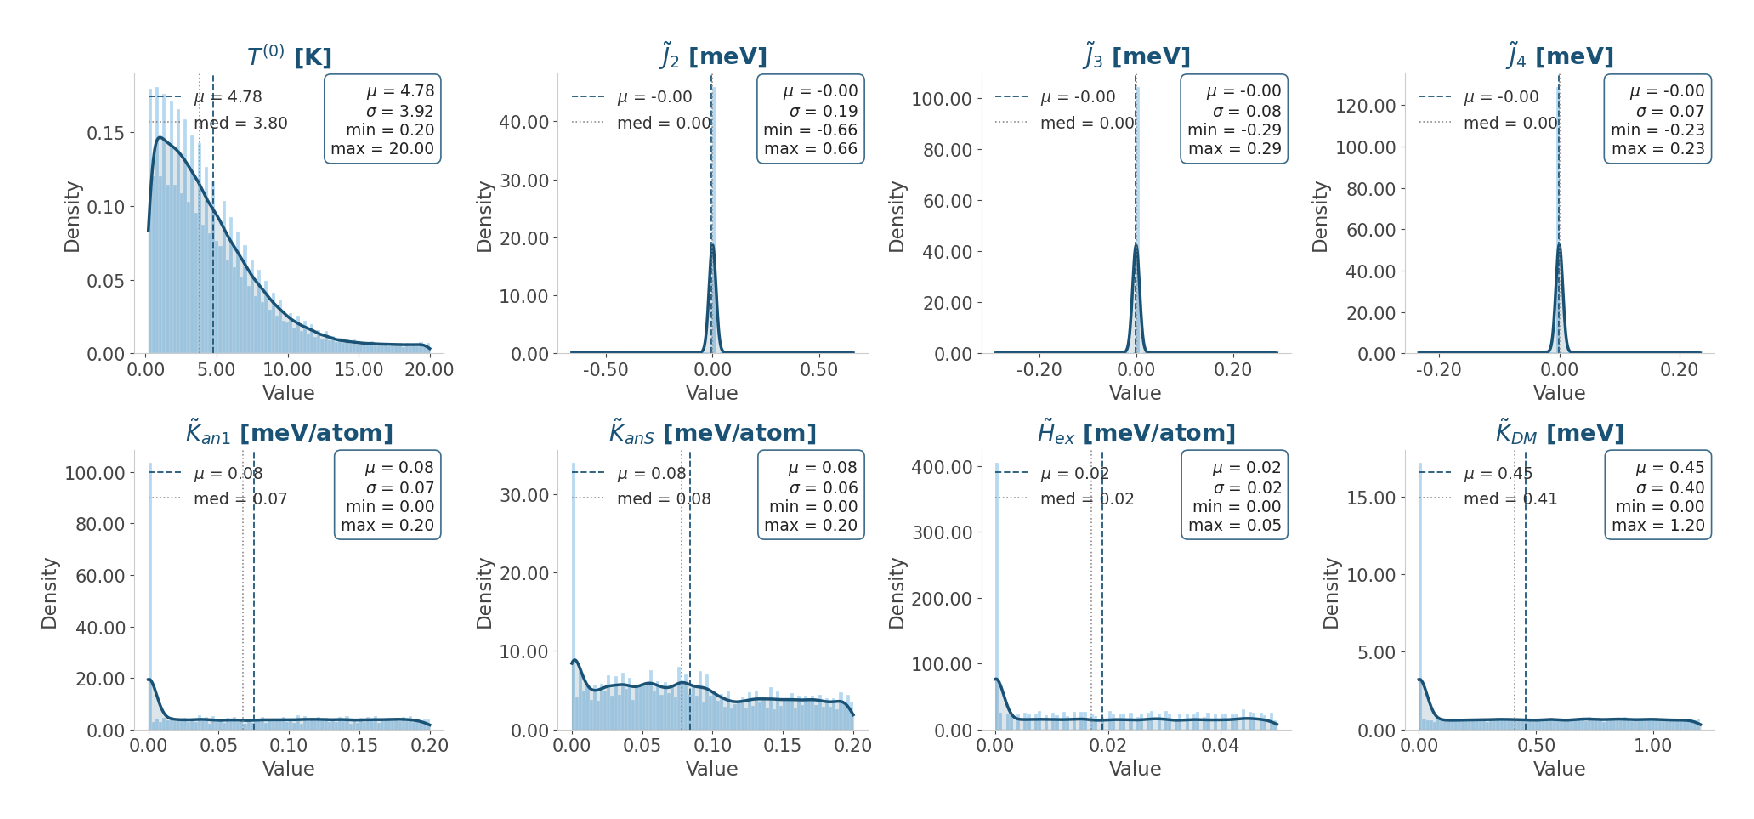
\includegraphics[width=\linewidth]{distributions}
    \caption{Empirical distributions of the thermodynamic and Hamiltonian parameters $\{T^{(0)}, \tilde{J}_2, \tilde{J}_3, \tilde{J}_4, \tilde{K}_{an1}, \tilde{K}_{anS}, \tilde{H}_{ex}, \tilde{K}_{DM}\}$ 
    used to generate the dataset. Each subplot presents a histogram and KDE for a given variable, along with 
    summary statistics including mean, standard deviation, and value range.}
    \label{fig:parameter_distributions}
\end{figure*}

%convergence monte carlo example
To further validate the physical consistency of the generated dataset and provide an intuitive understanding of the underlying spin dynamics, Figure~\ref{fig:convergence} illustrates the thermodynamic evolution of a representative magnetic nanodot during the Metropolis--Hastings Monte Carlo annealing process. This simulation is conducted under the fixed parameter configuration $\tilde{J}_1 = 1.0$~meV, $\tilde{J}_2 = \tilde{J}_3 = \tilde{J}_4 = 0.0$~meV, $\tilde{K}_{an1} = 0.10$~meV/atom, $\tilde{K}_{anS} = 0.00$~meV/atom, $\tilde{H}_{ex} = 0.00$~meV/atom, and $\tilde{K}_{DM} = 1.00$~meV, which constitutes a representative point within the full height-dimensional parameter space $\boldsymbol{\theta}$ defined in Table~\ref{tab:param_ranges}. The vanishing values of the higher-order exchange constants ($\tilde{J}_2$, $\tilde{J}_3$, $\tilde{J}_4$), surface anisotropy ($\tilde{K}_{anS}$), and external field ($\tilde{H}_{ex}$) isolate the dominant energetic competition between the first-shell symmetric exchange $\tilde{J}_1$ and the DMI $\tilde{K}_{DM}$, making this configuration particularly illustrative of the chiral ordering mechanism. The main panel tracks the total Hamiltonian energy $\mathcal{H}$ [meV] as a function of the exchange-normalized annealing temperature $T^{(0)}$ [K], while each inset displays the corresponding two-dimensional out-of-plane magnetization field $s_z$ of the central layer at that specific thermal state. At elevated temperatures ($T^{(0)} \gtrsim 15$~K), the spin configurations exhibit a fully disordered, paramagnetic character, manifesting as spatially uncorrelated fluctuations of $s_z$ with no preferred orientation. As the system is progressively cooled through the intermediate regime ($5~\text{K} \lesssim T^{(0)} \lesssim 15$~K), short-range correlated domains begin to nucleate, reflecting the growing dominance of the symmetric exchange interaction $\tilde{J}_1$ over thermal fluctuations. In this regime, the competition between $\tilde{J}_1$ and the $\tilde{K}_{DM}$ progressively induced non-collinear and chiral spin winding, visible as the emergence of alternating red-blue stripe-like patterns. Upon convergence to the near-ground state at $T^{(0)} = 0.1$~K, the system stabilizes into a well-defined labyrinthine domain configuration, characteristic of the helical phase governed by a strong DMI relative to the exchange energy. The monotonic decrease $\mathcal{H}$ throughout the annealing trajectory confirms the thermodynamic relaxation of the system toward \ch{a low-energy stable configuration}, validating the physical correctness of the Monte Carlo pipeline and the quality of the generated dataset as input for the deep learning regression framework.

%Monte carlo convergence
\begin{figure*}[t!]
    \centering
    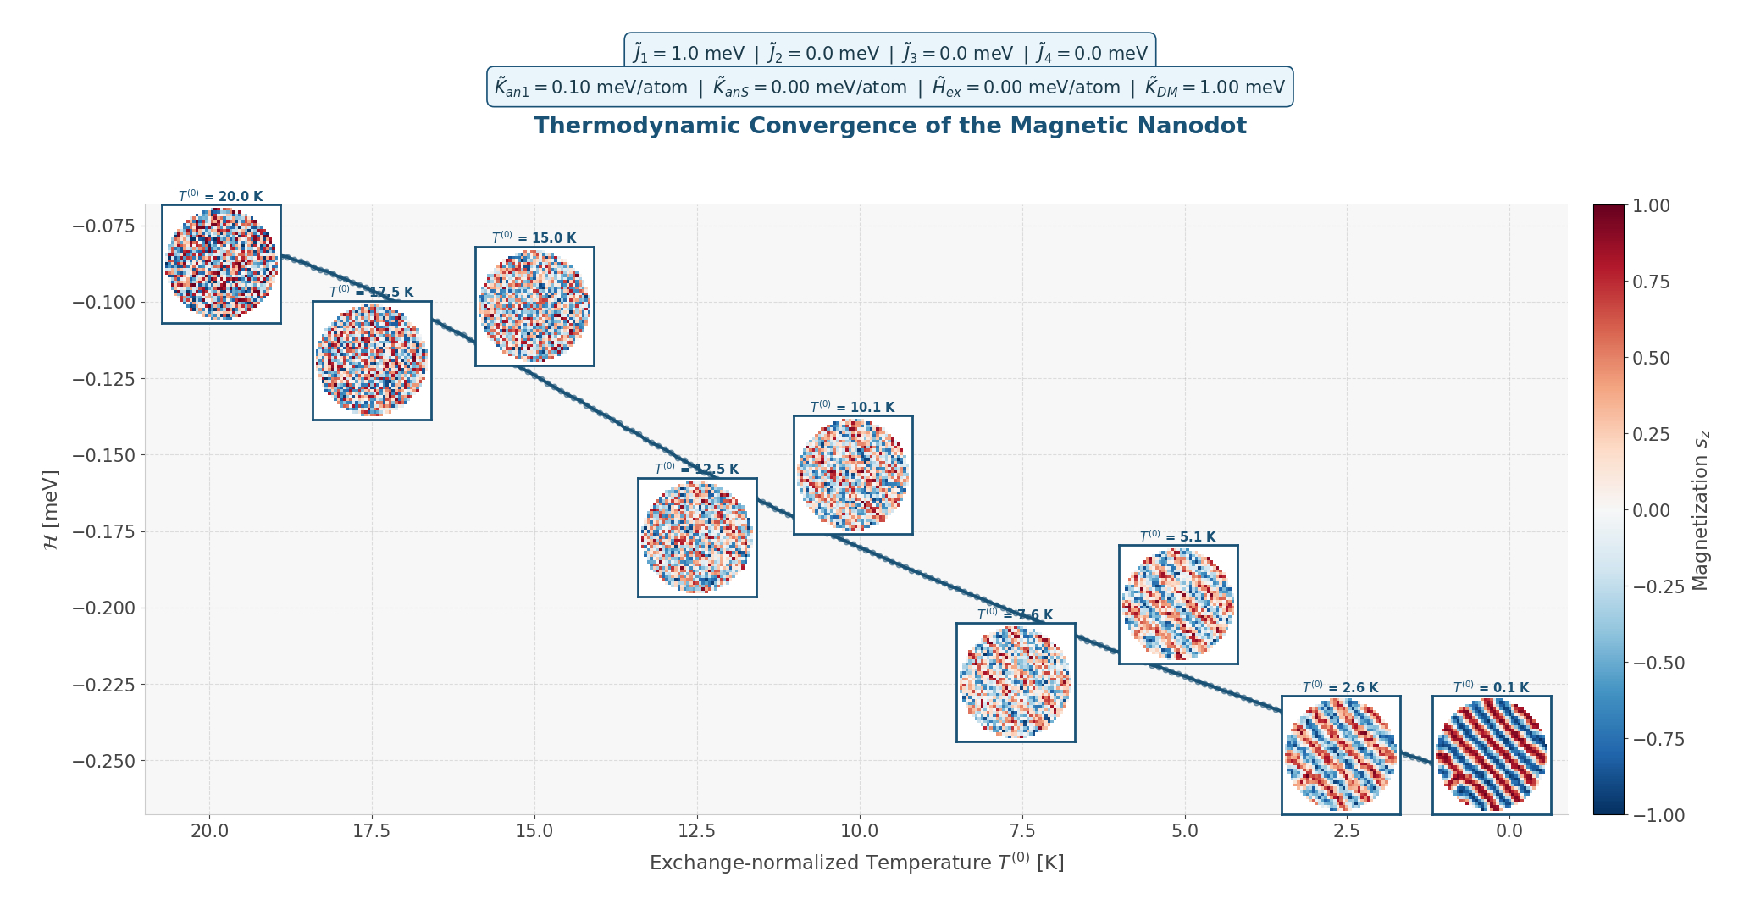
\includegraphics[width=\linewidth]{convergence}
    \caption{Thermodynamic convergence of a representative magnetic nanodot during simulated annealing. The main panel shows the total Hamiltonian energy $\mathcal{H}$ [meV] as a function of the exchange-normalized annealing temperature $T^{(0)}$ [K] under the fixed parameter configuration. Each inset depicts the 
    two-dimensional out-of-plane magnetization field $s_z$ of the central layer at the corresponding thermal state, illustrating the progressive transition from a fully disordered paramagnetic phase at high $T^{(0)}$ to a thermodynamically relaxed labyrinthine domain configuration at $T^{(0)} = 0.1$~K, driven by the competing energetic contributions of $\tilde{J}_1$ and $\tilde{K}_{DM}$.}
    \label{fig:convergence}
\end{figure*}

%2D and 3D configuration
Figure~\ref{fig:spin_configuration} illustrates the converged ground-state spin configuration of a magnetic nanodot at $T^{(0)}_{final}=0.1$~K, simulated with specific fixed parameters ($\tilde{J}_1=1.0$~meV, $\tilde{K}_{DM}=1.00$~meV, $\tilde{K}_{an1}=0.10$~meV/atom, and all other parameters zeroed; see Table~\ref{tab:param_ranges}). Panel~(a) maps the 2D out-of-plane magnetization ($s_z$) on the central layer---using dots for out-of-plane moments and arrows for transverse components---while Panel~(b) displays the full 3D volumetric spin texture. The nanodot exhibits a labyrinthine domain pattern characterized by chiral walls. This morphology is driven directly by the energetic competition between the ferromagnetic symmetric exchange ($\tilde{J}_1$) and the DMI ($\tilde{K}_{DM}$). With a ratio of $\tilde{K}_{DM}/\tilde{J}_1=1.0$, the system stabilizes in the helical phase. By nullifying higher-order exchange, surface anisotropy, and external fields, this $\tilde{J}_1$--$\tilde{K}_{DM}$ competition is fully isolated, allowing the stripe-like domains to develop freely without preferential axial pinning.

%2D and 3D configuration
\begin{figure*}[t!]
    \centering
    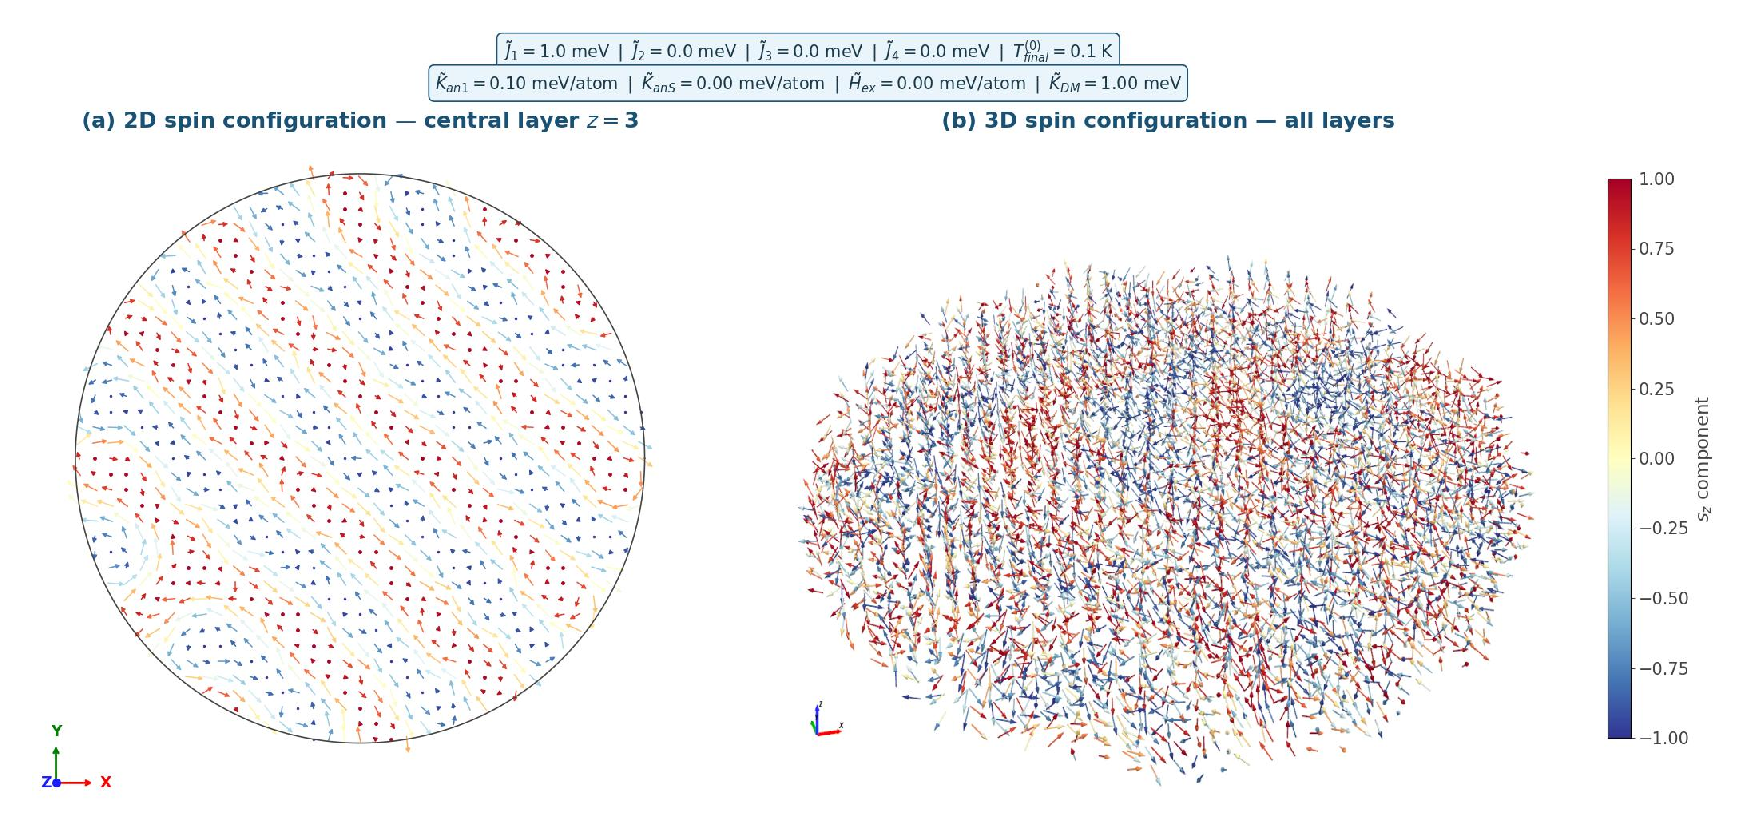
\includegraphics[width=\linewidth]{3D}
    \caption{Converged ground-state spin configuration of a representative magnetic nanodot at $T^{(0)}_{final} = 0.1$~K under a fixed parameter configuration. (a)~Two-dimensional projection of the out-of-plane magnetization field $s_z$: colored dots indicate spins oriented predominantly out-of-plane, while colored arrows represent the in-plane orientation $(s_x, s_y)$ of transverse moments. (b)~Full three-dimensional spin configuration, revealing the volumetric coherence of the labyrinthine chiral domain structure stabilized by the competition between $\tilde{J}_1$ and $\tilde{K}_{DM}$. Color encodes the $s_z$ component.}
    \label{fig:spin_configuration}
\end{figure*}

Now, to fully characterize the structural diversity generated by the Monte Carlo annealing protocol across the entire dataset, Figure~\ref{fig:phase_diagrams} presents two-dimensional phase diagrams of the magnetization image as a function of key Hamiltonian parameter pairs: $T^{(0)}$ versus $\tilde{J}_2$ and $T^{(0)}$ versus $\tilde{K}_{DM}$. These diagrams illustrate the macroscopic topological transitions driven by the underlying atomistic energetic competition. At elevated annealing temperatures, specifically above the effective Curie temperature $T_C$, thermal fluctuations overwhelm the magnetic interactions, collapsing all configurations into an indistinguishable, highly degenerate paramagnetic noise phase regardless of the specific exchange or DMI strengths. Conversely, in the low-temperature regime, the system stabilizes into ordered states, revealing distinct boundaries between chiral, ferromagnetic, and antiferromagnetic phases. Notably, the phase diagrams expose critical transition zones---such as the boundary between chiral and disordered states near $\tilde{K}_{DM} \approx 0$ meV, and the sign transition near $\tilde{J}_2 \approx 0$ meV---where disparate parameter combinations yield visually overlapping spatial textures. By comprehensively sampling this phase space, the thermodynamic simulation establishes a highly diverse and structurally ambiguous dataset (ill-conditioned mapping), setting a rigorously challenging foundation for the subsequent inverse deep learning parameter estimation.


\begin{figure*}[t!]
    \centering
    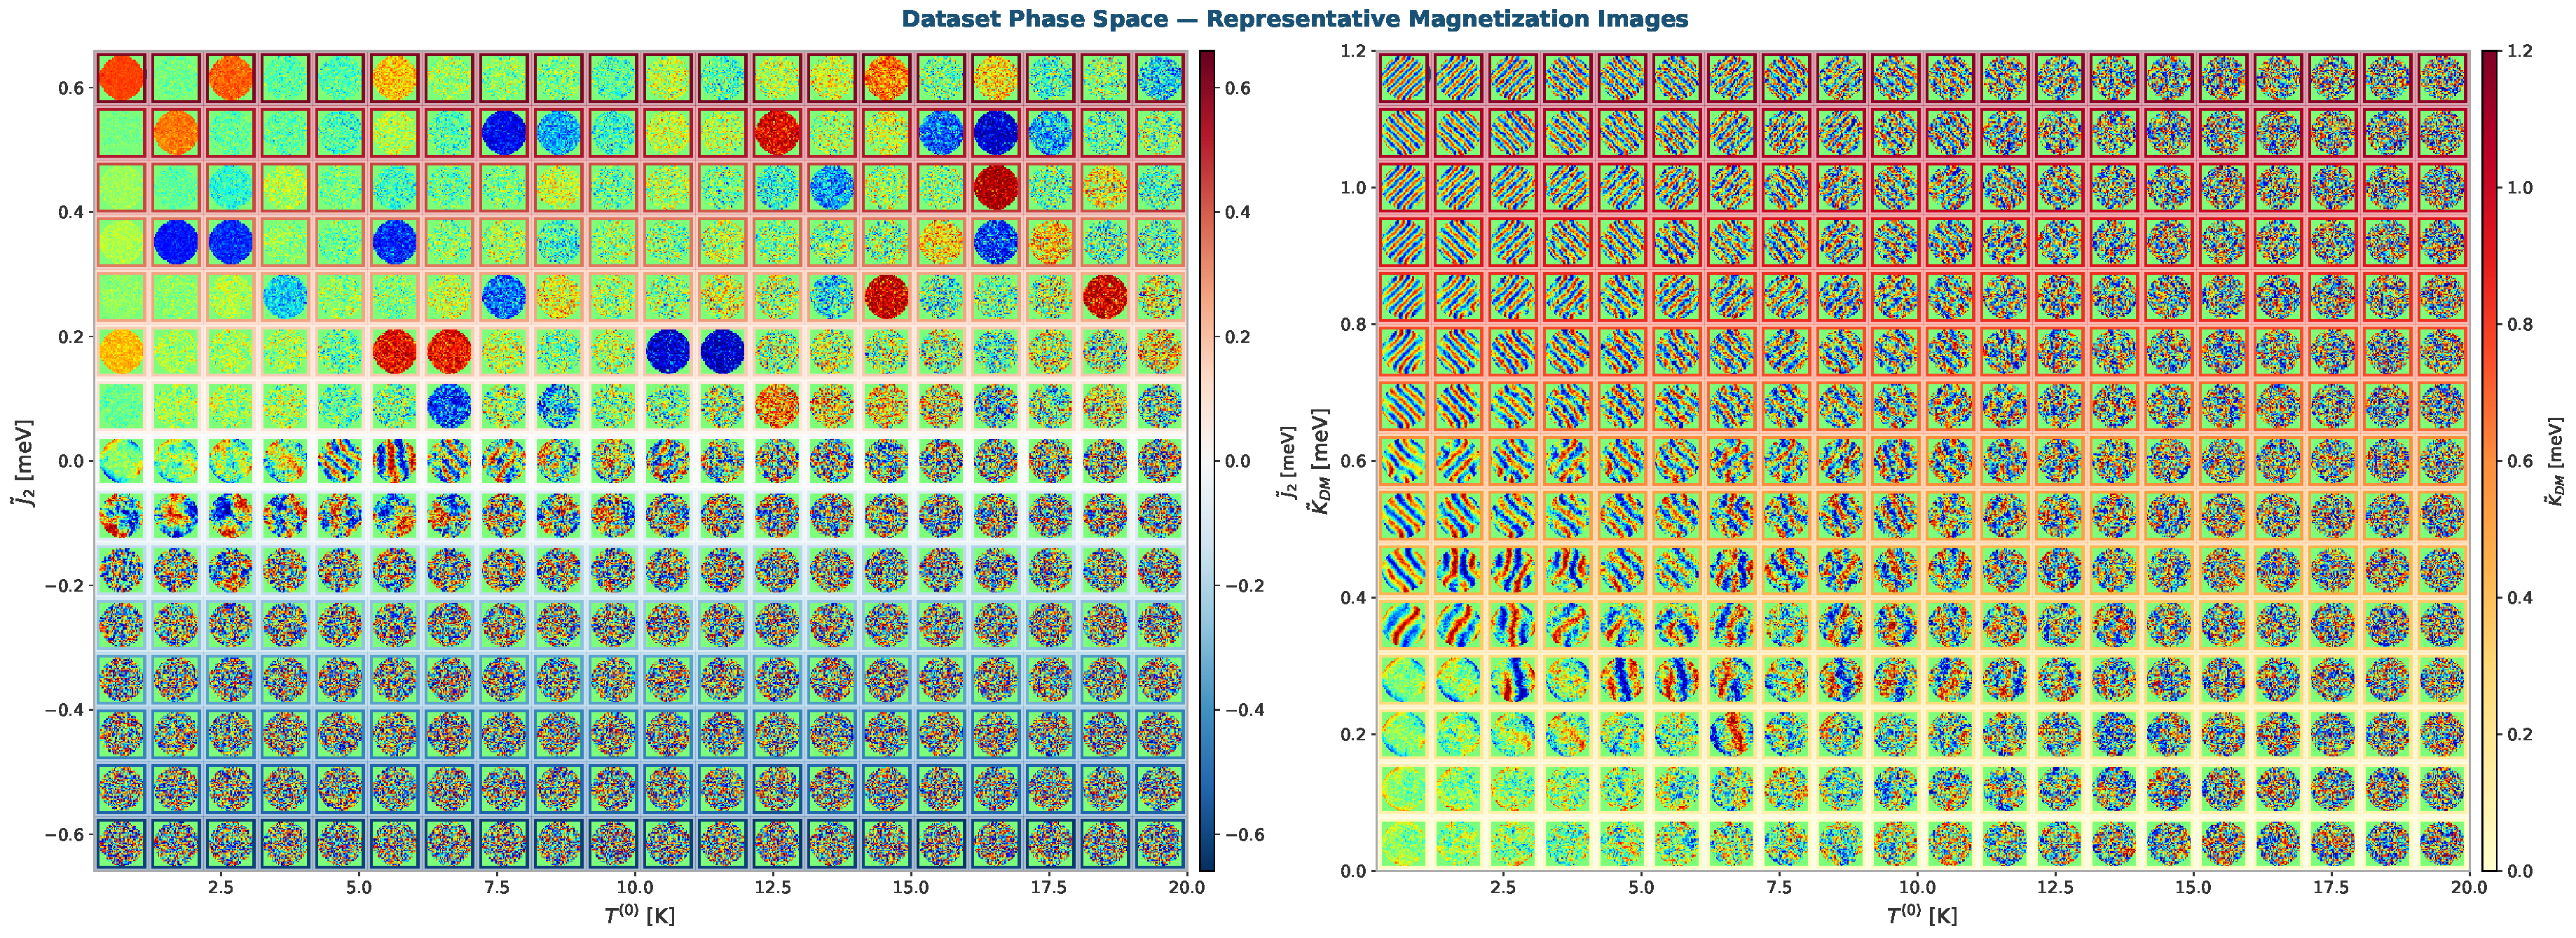
\includegraphics[width=\linewidth]{dataset}
    \caption{Two-dimensional phase diagrams of the magnetization 
    texture $\mathbf{X}_n$ as a function of pairs of Hamiltonian 
    parameters. \textbf{(a)}~$T^{(0)}$ vs $\tilde{J}_2$. 
    \textbf{(b)}~$T^{(0)}$ vs $\tilde{K}_{DM}$. Each cell 
    displays a representative magnetization image sampled from the 
    dataset at the corresponding parameter combination; background 
    color encodes the value of the vertical-axis parameter.}
    \label{fig:phase_diagrams}
\end{figure*}


\subsection{Deep Learning Regression Results}\label{sec:dl_results}

The predictive performance of the studied architectures (DenseNet,
ResNet, Xception, and ViT) was assessed on the held-out test set
comprising 15\% of the total dataset. Each model was tasked with
simultaneously inferring the complete extended parameter vector
$\boldsymbol{\theta}$ directly from the two-dimensional out-of-plane
magnetization image $\mathbf{X}_n$, without any auxiliary physical
information. As shown in Figures~\ref{fig:r2_metrics}
and~\ref{fig:mae_metrics}, no single architecture uniformly dominates
both metrics: the ViT attains the highest $R^2$ score for seven of the
eight Hamiltonian parameters ($T^{(0)}$, $\tilde{J}_3$, $\tilde{J}_4$,
$\tilde{K}_{an1}$, $\tilde{K}_{anS}$, $\tilde{H}_{ex}$, and
$\tilde{K}_{DM}$), while Xception achieves the highest $R^2$ for the
second-shell exchange constant $\tilde{J}_2$. Notably, despite the ViT's superior variance-explained
performance, Xception consistently produces the lowest Mean Absolute
Error across most parameters, including $T^{(0)}$, $\tilde{J}_2$,
$\tilde{J}_3$, $\tilde{J}_4$, $\tilde{H}_{ex}$, and $\tilde{K}_{DM}$,
whereas the ViT only minimizes the MAE for the anisotropy constants
$\tilde{K}_{an1}$ and $\tilde{K}_{anS}$. This complementary behavior
between $R^2$ and MAE indicates that, while the ViT captures a larger
fraction of the parameter variance and is therefore more sensitive
to the long-range correlations governing global magnetic order
Xception yields tighter absolute predictions in the dense ordered
regions of the parameter space, where local spatial structure is the
dominant predictive signal. The ViT's broad advantage in $R^2$ is
physically interpretable: by processing the magnetization field
$\mathbf{X}_n$ as a sequence of non-overlapping spatial patches and
computing multi-head self-attention scores across all patch pairs, the
ViT explicitly captures long-range correlations between distant spin
textures, such as the global chirality imposed by $\tilde{K}_{DM}$
and the large-scale ordering driven by $\tilde{J}_1$, that are
fundamentally inaccessible to purely local convolutional receptive
fields. Xception's competitive behavior, in turn, stems from its
depthwise separable convolution mechanism, which efficiently decouples
the extraction of spatial spin-texture frequencies from the
cross-channel correlations required to map those features onto the
Hamiltonian parameter space, yielding the most accurate point
predictions for the dominantly identifiable parameters.

Figures~\ref{fig:r2_metrics} and~\ref{fig:mae_metrics} reveal a
pronounced and physically interpretable heterogeneity in predictive
accuracy across the parameter space. The initial annealing temperature
$T^{(0)}$, the second-shell exchange constant $\tilde{J}_2$, and the
DMI strength $\tilde{K}_{DM}$ consistently yield the highest $R^2$
scores across all architectures, reflecting the robust and spatially
distinctive topological imprints they leave on the observable
magnetization texture: $T^{(0)}$ governs the global degree of spin
order, $\tilde{J}_2$ controls the second-neighbor exchange pathway
that modulates the domain-scale collinearity, and $\tilde{K}_{DM}$
directly dictates the characteristic wavelength and chirality of the
domain patterns. However, a seemingly contradictory observation
emerges when examining the MAE panels in Figure~\ref{fig:mae_metrics}:
despite their high $R^2$ scores, $T^{(0)}$, $\tilde{J}_2$, and
$\tilde{K}_{DM}$ also exhibit comparatively larger absolute errors in
their respective physical units --- reaching up to approximately
$1.0\,\mathrm{K}$ for $T^{(0)}$, $0.065\,\mathrm{meV}$ for
$\tilde{J}_2$, and $0.05\,\mathrm{meV}$ for $\tilde{K}_{DM}$ in the
worst-performing architecture. This apparent inconsistency is not a
failure of the models but rather a direct consequence of the
thermodynamic landscape of the dataset. As illustrated in the phase
diagrams of Figure~\ref{fig:phase_diagrams}, the parameter space
contains extensive high-temperature regions where thermal
fluctuations above the effective Curie temperature $T_C$ collapse the
magnetization texture into an indistinguishable paramagnetic noise
phase, regardless of the specific values of $\tilde{J}_2$ or
$\tilde{K}_{DM}$. Within these thermally disordered regimes, visually
identical configurations correspond to widely different parameter
values, rendering the inverse mapping fundamentally ill-posed and
inflating the absolute prediction error even when the global
correlation structure --- captured by $R^2$ --- remains strong. The
MAE values for $T^{(0)}$, $\tilde{J}_2$, and $\tilde{K}_{DM}$
therefore reflect the intrinsic degeneracy of the high-temperature
paramagnetic phase rather than a systematic modeling deficiency: the
same parameter that is most accurately recovered in the ordered
low-temperature regime (where the spin texture preserves a clear
topological signature) is simultaneously the most degenerate in the
disordered high-temperature regime (where the texture collapses into
noise), producing non-negligible global MAE values driven primarily
by the ill-conditioned subset of the dataset. A rigorous quantitative
decomposition of this effect requires first separating the dataset
into its constituent magnetic structural categories, as the global
aggregation of all configurations inevitably conflates high-accuracy
ordered-phase predictions with fundamentally ill-posed
paramagnetic-regime estimates. This per-phase analysis is addressed
further ahead, where the unsupervised structural clustering of the
magnetization images allows us to isolate and quantify the specific
contribution of each magnetic phase to the observed prediction error.

Conversely, the models exhibit two qualitatively distinct regimes of
limited predictive performance for the remaining Hamiltonian
parameters, which together delimit the fundamental identifiability
boundaries of the inverse problem in the 2D observation space. The
higher-order exchange constants $\tilde{J}_3$ and $\tilde{J}_4$
constitute the most severe case: their $R^2$ scores remain near zero
across all evaluated architectures, indicating that the models are
unable to recover meaningful information about these parameters
beyond the dataset mean. Physically, the spatial signatures of these
subordinate exchange constants are energetically dominated by the
primary $\tilde{J}_1$ and $\tilde{J}_2$ interactions, progressively
masking their observable effect on the magnetization texture and
rendering them effectively unidentifiable from the $s_z$ projection
alone. Notably, however, their MAE values --- on the order of
$0.03$--$0.05\,\mathrm{meV}$ --- remain numerically comparable to
those of the better-identified parameters, which is a direct
consequence of their narrow physical range in the dataset rather than
genuine predictive skill: a model predicting the dataset mean for
$\tilde{J}_3$ and $\tilde{J}_4$ will naturally incur a small absolute
error simply because the dynamic range of these parameters is itself
limited. The magnetocrystalline anisotropy constants $\tilde{K}_{an1}$
and $\tilde{K}_{anS}$ together with the external Zeeman field
$\tilde{H}_{ex}$, in turn, occupy an intermediate identifiability
regime. This partial predictability is physically consistent: these
parameters couple primarily to the in-plane spin components $s_x$
and $s_y$ rather than to the observable out-of-plane component
$s_z$, so the models are able to recover them only indirectly through
the secondary topological imprints they induce on the chiral domain
structure, such as the modulation of stripe periodicity or the
preferential orientation of skyrmion cores. Furthermore, the visual
manifestations of surface anisotropy $\tilde{K}_{anS}$ remain
partially entangled with bulk anisotropy $\tilde{K}_{an1}$ and
geometrically confined to the boundary layer of the nanodot, while
the Zeeman contribution $\tilde{H}_{ex}$ --- with MAE values below
$0.009\,\mathrm{meV/atom}$ across all architectures --- becomes
increasingly indistinguishable from thermal disorder in the
high-temperature regime. Together, these effects render the anisotropy
and field parameters intrinsically partially observable and define the
fundamental identifiability limits of the inverse problem within the
two-dimensional $s_z$ projection.

\begin{figure*}[t!]
    \centering
    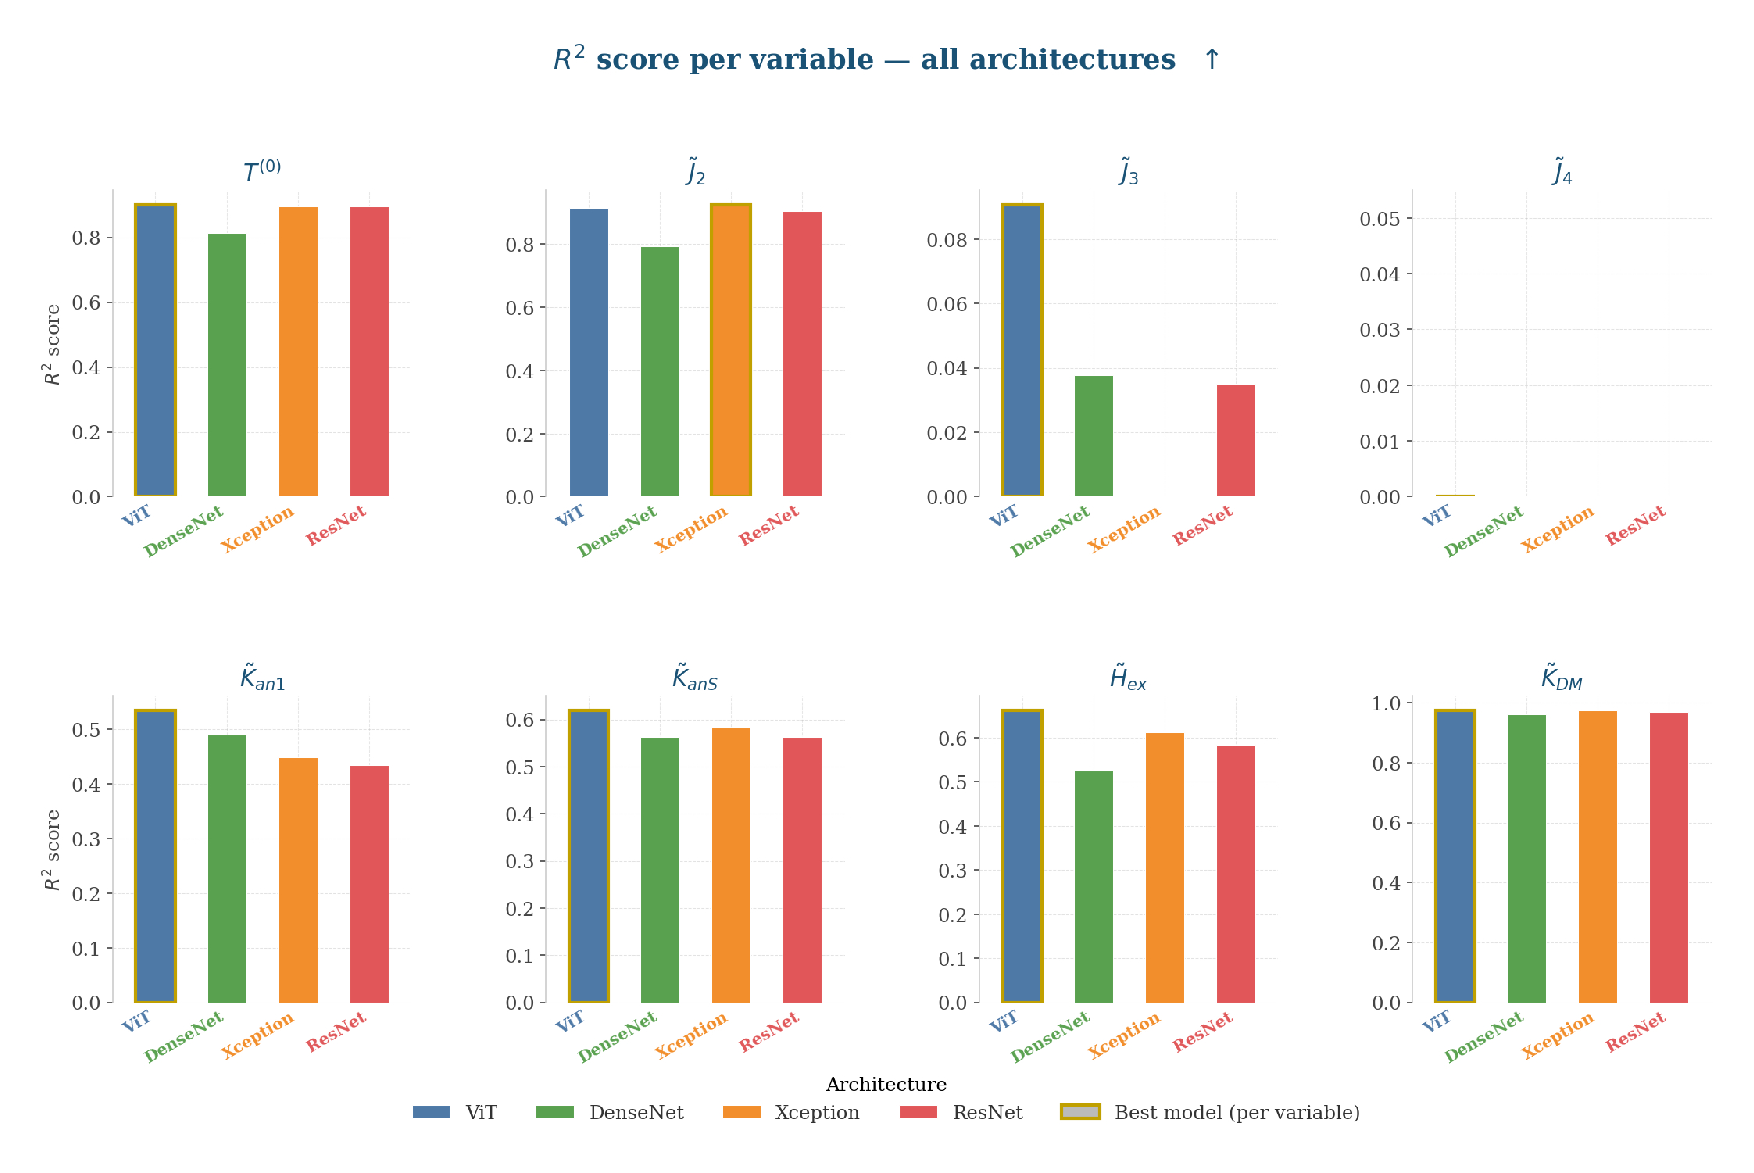
\includegraphics[width=\linewidth]
    {r2_metrics}
    \caption{Per-variable $R^2$ score across all evaluated 
    architectures for the eight Hamiltonian parameters 
    $\boldsymbol{\theta}$, reported on the held-out test set. Each 
    panel corresponds to one target parameter and shows one bar per 
    architecture. Negative $R^2$ values, 
    indicating predictions no better than the dataset mean, are 
    clipped to zero for visualization clarity. Gold-bordered bars 
    indicate the best-performing architecture for each parameter.}
    \label{fig:r2_metrics}
\end{figure*}

\begin{figure*}[t!]
    \centering
    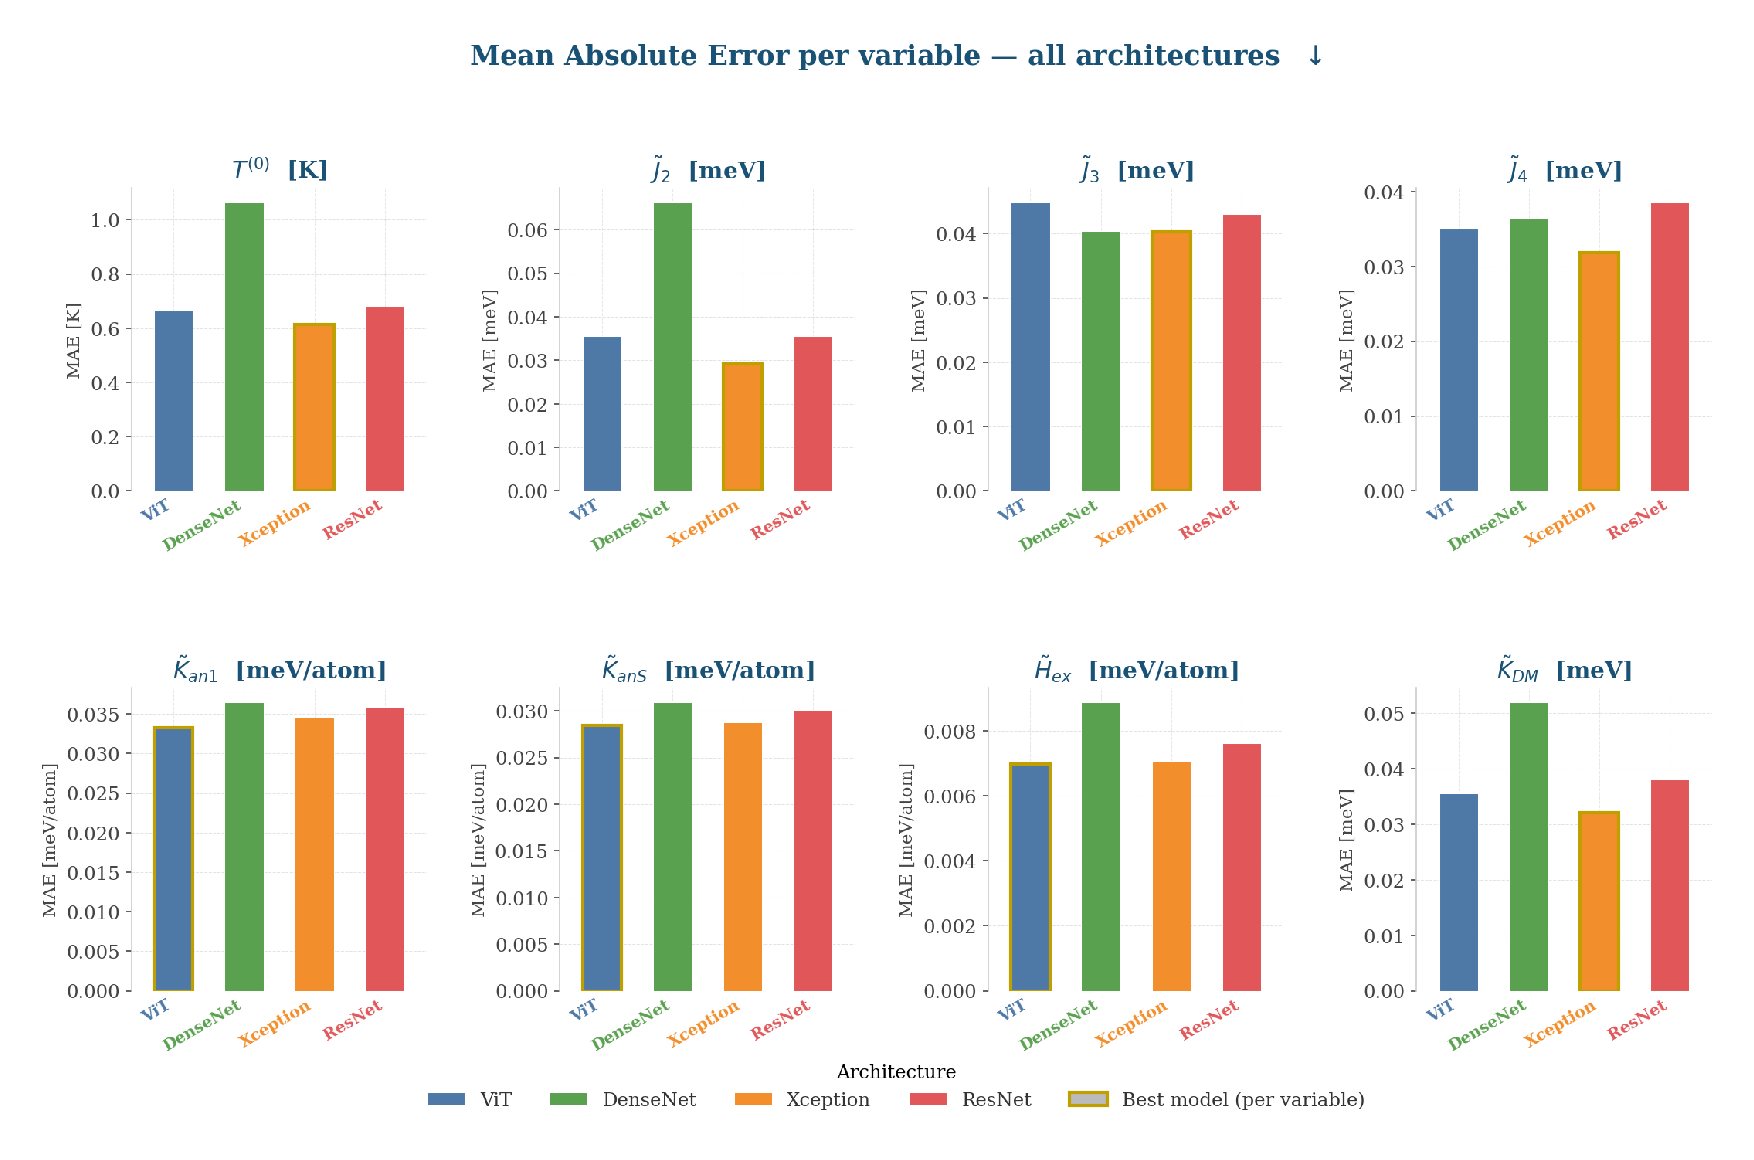
\includegraphics[width=0.75\linewidth]
    {mae_metrics}
    \caption{Per-variable Mean Absolute Error (MAE) across all
    evaluated architectures for the eight Hamiltonian parameters
    $\boldsymbol{\theta}$, reported on the held-out test set in the
    original physical units of each parameter (K for $T^{(0)}$, meV
    for exchange and DMI constants, and meV/atom for anisotropy and
    external field parameters). Each panel corresponds to one target
    parameter and shows one bar per architecture. The comparatively
    larger MAE observed for $T^{(0)}$, $\tilde{J}_2$, and
    $\tilde{K}_{DM}$ --- reaching up to $1.0\,\mathrm{K}$,
    $0.065\,\mathrm{meV}$, and $0.05\,\mathrm{meV}$ respectively in
    the worst-performing architecture --- is attributable to the
    thermally disordered paramagnetic configurations populating the
    high-temperature regime of the dataset (see
    Figure~\ref{fig:phase_diagrams}), where visually identical
    textures correspond to widely different parameter values,
    rendering the inverse mapping fundamentally ill-posed even when
    the global $R^2$ correlation remains strong. The comparatively
    small MAE of $\tilde{J}_3$ and $\tilde{J}_4$ despite their
    near-zero $R^2$ reflects the narrow dynamic range of these
    parameters in the dataset rather than genuine predictive skill.
    Gold-bordered bars indicate the best-performing architecture
    for each parameter.}
    \label{fig:mae_metrics}
\end{figure*}

%umap visualization
To gain deeper insight into the internal representations learned by 
the ViT during the inverse Hamiltonian estimation task, 
Figure~\ref{fig:umap_latent} presents a Uniform Manifold 
Approximation and Projection (UMAP) of the model's latent 
space~\cite{ghojogh2021uniform}, where each point corresponds to a 
test sample colored by the value of each of the eight Hamiltonian 
parameters $\boldsymbol{\theta}$. The UMAP embedding was computed 
from the high-dimensional feature vectors extracted from the ViT's 
final encoder block prior to the regression head, providing a 
two-dimensional visualization of the geometric structure that the 
model has learned to impose on the magnetization image manifold. 
Rather than forming a single undifferentiated cloud, the latent 
space exhibits a rich topological structure composed of several 
geometrically distinct clusters and continuous gradients, reflecting 
the fact that the model has organized the magnetization textures 
according to their underlying physical regimes. Examining the 
coloring by $T^{(0)}$ reveals the clearest and most spatially 
coherent gradient across the embedding: low-temperature ordered 
configurations concentrate in well-separated compact regions, while 
high-temperature disordered states occupy a large, diffuse cluster 
in the upper portion of the latent space, consistent with the strong 
predictive performance of the model on $T^{(0)}$. The DMI strength 
$\tilde{K}_{DM}$ also produces a structured gradient in the latent 
space, with high-$\tilde{K}_{DM}$ helical configurations forming a 
distinct elongated region separated from the low-$\tilde{K}_{DM}$ 
disordered states, confirming that the ViT has successfully encoded 
the chiral winding imposed by the DMI as a geometrically meaningful 
direction in its latent representation. In contrast, the 
longer-range exchange constants $\tilde{J}_3$ and $\tilde{J}_4$ 
produce nearly uniform colorings across the entire embedding, 
indicating that the model's internal representations carry little 
discriminative information about these parameters a result that 
is fully consistent with their low $R^2$ values and their energetic 
subordination to the dominant first-shell exchange 
$\tilde{J}_1 = 1.0$~meV. Similarly, the anisotropy constants 
$\tilde{K}_{an1}$ and $\tilde{K}_{anS}$ and the external field 
$\tilde{H}_{ex}$ show spatially mixed and unstructured colorings, 
corroborating the partial observability limitations and the 
confounding effects identified in the regression analysis.

%umap 2D
To further investigate the physical organization of the ViT's 
latent representations, a structured clustering analysis was 
conducted directly on the two-dimensional UMAP embedding of the 
test set feature vectors. Prior to visualization, the raw UMAP 
coordinates were normalized to the unit interval $[0,1]$ along 
each axis using a min-max transformation. The spatial distribution 
of magnetization images across the normalized latent space, 
illustrated in Figure~\ref{fig:umap_images_only}, reveals that 
the Vision Transformer has organized the magnetization textures 
into geometrically distinct and physically interpretable regions 
without any explicit supervision of magnetic phase labels. The 
lower-left region of the embedding is occupied by ordered, 
low-temperature spin configurations exhibiting well-defined 
helical stripe and labyrinthine domain patterns, whose spatial 
periodicity and chiral winding angle vary continuously along 
the diagonal axis of the manifold --- a direct reflection of 
the systematic variation of $\tilde{K}_{DM}$ and $T^{(0)}$ 
within this phase. The upper central region concentrates 
thermally disordered configurations with increasing paramagnetic 
noise, consistent with samples at high $T^{(0)}$ where thermal 
fluctuations dominate over the competing energetic contributions 
of $\tilde{J}_1$ and $\tilde{K}_{DM}$. The isolated cluster 
visible in the upper-right corner of the embedding corresponds 
to a qualitatively distinct topological regime --- ferromagnetic 
and skyrmion-like configurations with uniform or radially 
symmetric $s_z$ distributions --- whose geometric separation 
from the main manifold confirms that the Vision Transformer has 
successfully encoded these structures as a fundamentally 
different category of spin texture in its latent space.

%UMAP ViT
\begin{figure*}[t!]
    \centering
    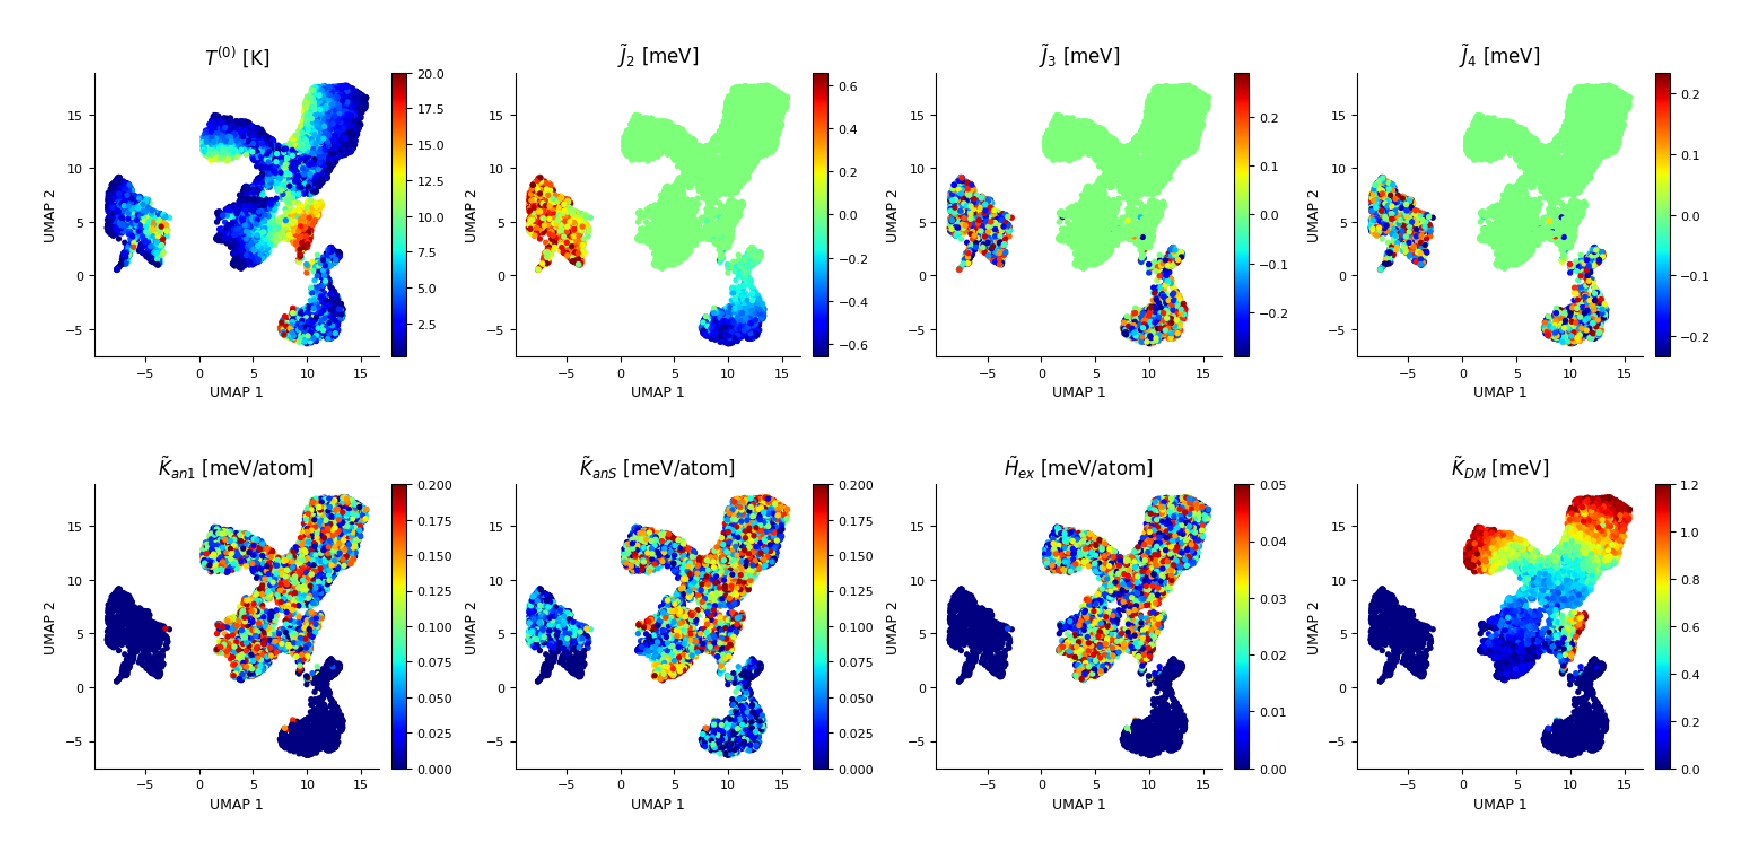
\includegraphics[width=\linewidth]
    {umap_latent}
    \caption{UMAP-based 2D projection of the ViT latent space 
    on the held-out test set, colored by each of the eight 
    Hamiltonian parameters $\boldsymbol{\theta} = [T^{(0)}, 
    \tilde{J}_2, \tilde{J}_3, \tilde{J}_4, \tilde{K}_{an1}, 
    \tilde{K}_{anS}, \tilde{H}_{ex}, \tilde{K}_{DM}]$. Each 
    point represents a magnetization image $\mathbf{X}_n$ 
    projected from the high-dimensional feature space of the 
    final Transformer encoder block into two dimensions via UMAP.}
    \label{fig:umap_latent}
\end{figure*}

%umap 2D
\begin{figure*}[t!]
    \centering
    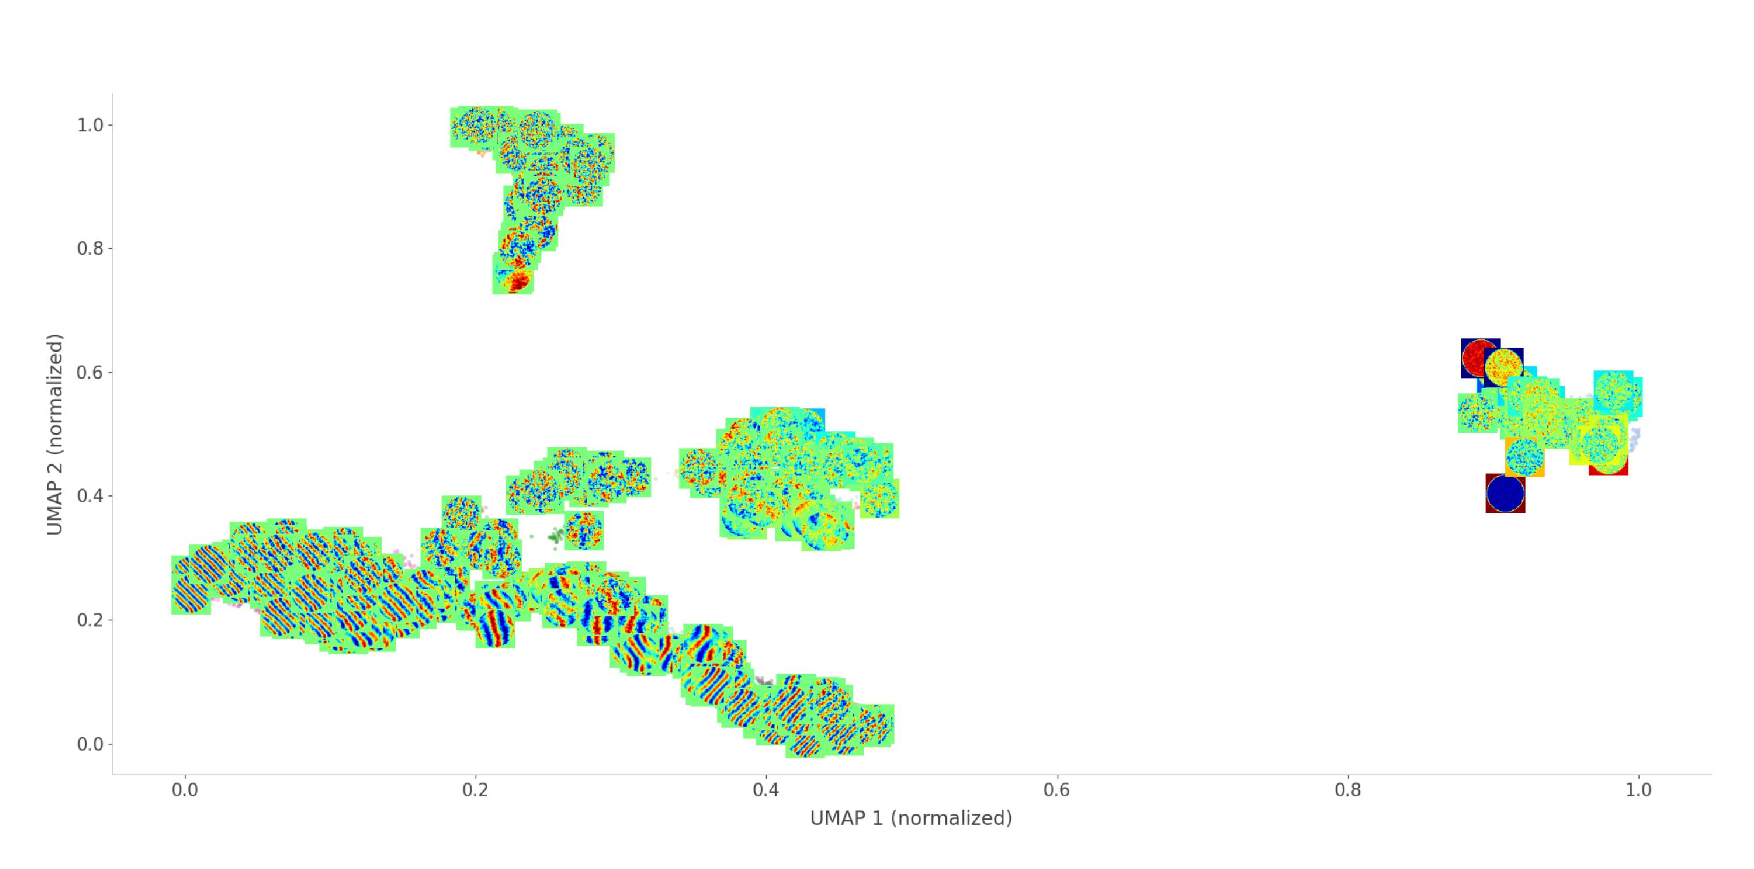
\includegraphics[width=\linewidth]
    {umap_images_only}
    \caption{Spatial distribution of magnetization images $\mathbf{X}_n$ across the normalized two-dimensional UMAP projection of the ViT latent space (test set). Both axes are normalized to $[0,1]$. Each thumbnail represents the out-of-plane magnetization field $s_z$ of a randomly selected test sample placed at its corresponding normalized UMAP coordinate.}
    \label{fig:umap_images_only}
\end{figure*}

To systematically identify and characterize the dominant magnetic 
phases encoded in the latent space, a density-based clustering 
analysis was performed using the HDBSCAN algorithm on the UMAP 
embedding, followed by a KMeans subdivision of anomalously large 
clusters. Based on visual inspection of representative samples 
and the mean values of the Hamiltonian parameters 
$\boldsymbol{\theta}$ within each group, the resulting clusters 
were consolidated into four physically meaningful magnetic phase 
categories.

The \textit{ferromagnetic phase} groups configurations characterized by near-uniform out-of-plane magnetization distributions, where the spins are predominantly aligned along a single direction with minimal spatial modulation, reflecting the dominance of ferromagnetic exchange interactions over chiral and thermal perturbations. The \textit{others} category constitutes the most heterogeneous group in the dataset, gathering configurations that do not exhibit the defining spatial signatures of any single ordered magnetic phase. This category encompasses thermally disordered states in which thermal fluctuations have disrupted long-range spin order, transitional configurations located at the boundaries between competing phases, and topologically mixed textures whose spatial structure is ambiguous or intermediate between ordered regimes. The common characteristic of all configurations in this group is the absence of a distinctive and reproducible magnetization pattern, making them the most structurally ill-conditioned samples in the dataset. The \textit{labyrinthine \& conical phase} comprises configurations exhibiting well-defined, spatially extended stripe and labyrinthine domain patterns with clear periodicity and chiral winding, reflecting the stabilization of competing magnetic interactions into ordered mesoscopic textures at sufficiently low annealing temperatures. Finally, the \textit{helical phase} contains the most spatially coherent and regularly ordered configurations in the dataset, displaying well-defined helical stripe patterns with consistent chiral winding direction and spatial periodicity across the entire nanodot, representing the most energetically ordered magnetic ground states accessible within the sampled parameter space.

Figure~\ref{fig:structure_representatives} presents five 
representative magnetization images per phase, selected as the 
samples closest to the centroid of each group in the UMAP 
embedding, along with the mean Hamiltonian parameters 
$\langle T^{(0)}\rangle$, $\langle\tilde{J}_2\rangle$, and 
$\langle\tilde{K}_{DM}\rangle$ characterizing each phase.

\begin{figure*}[t!]
    \centering
    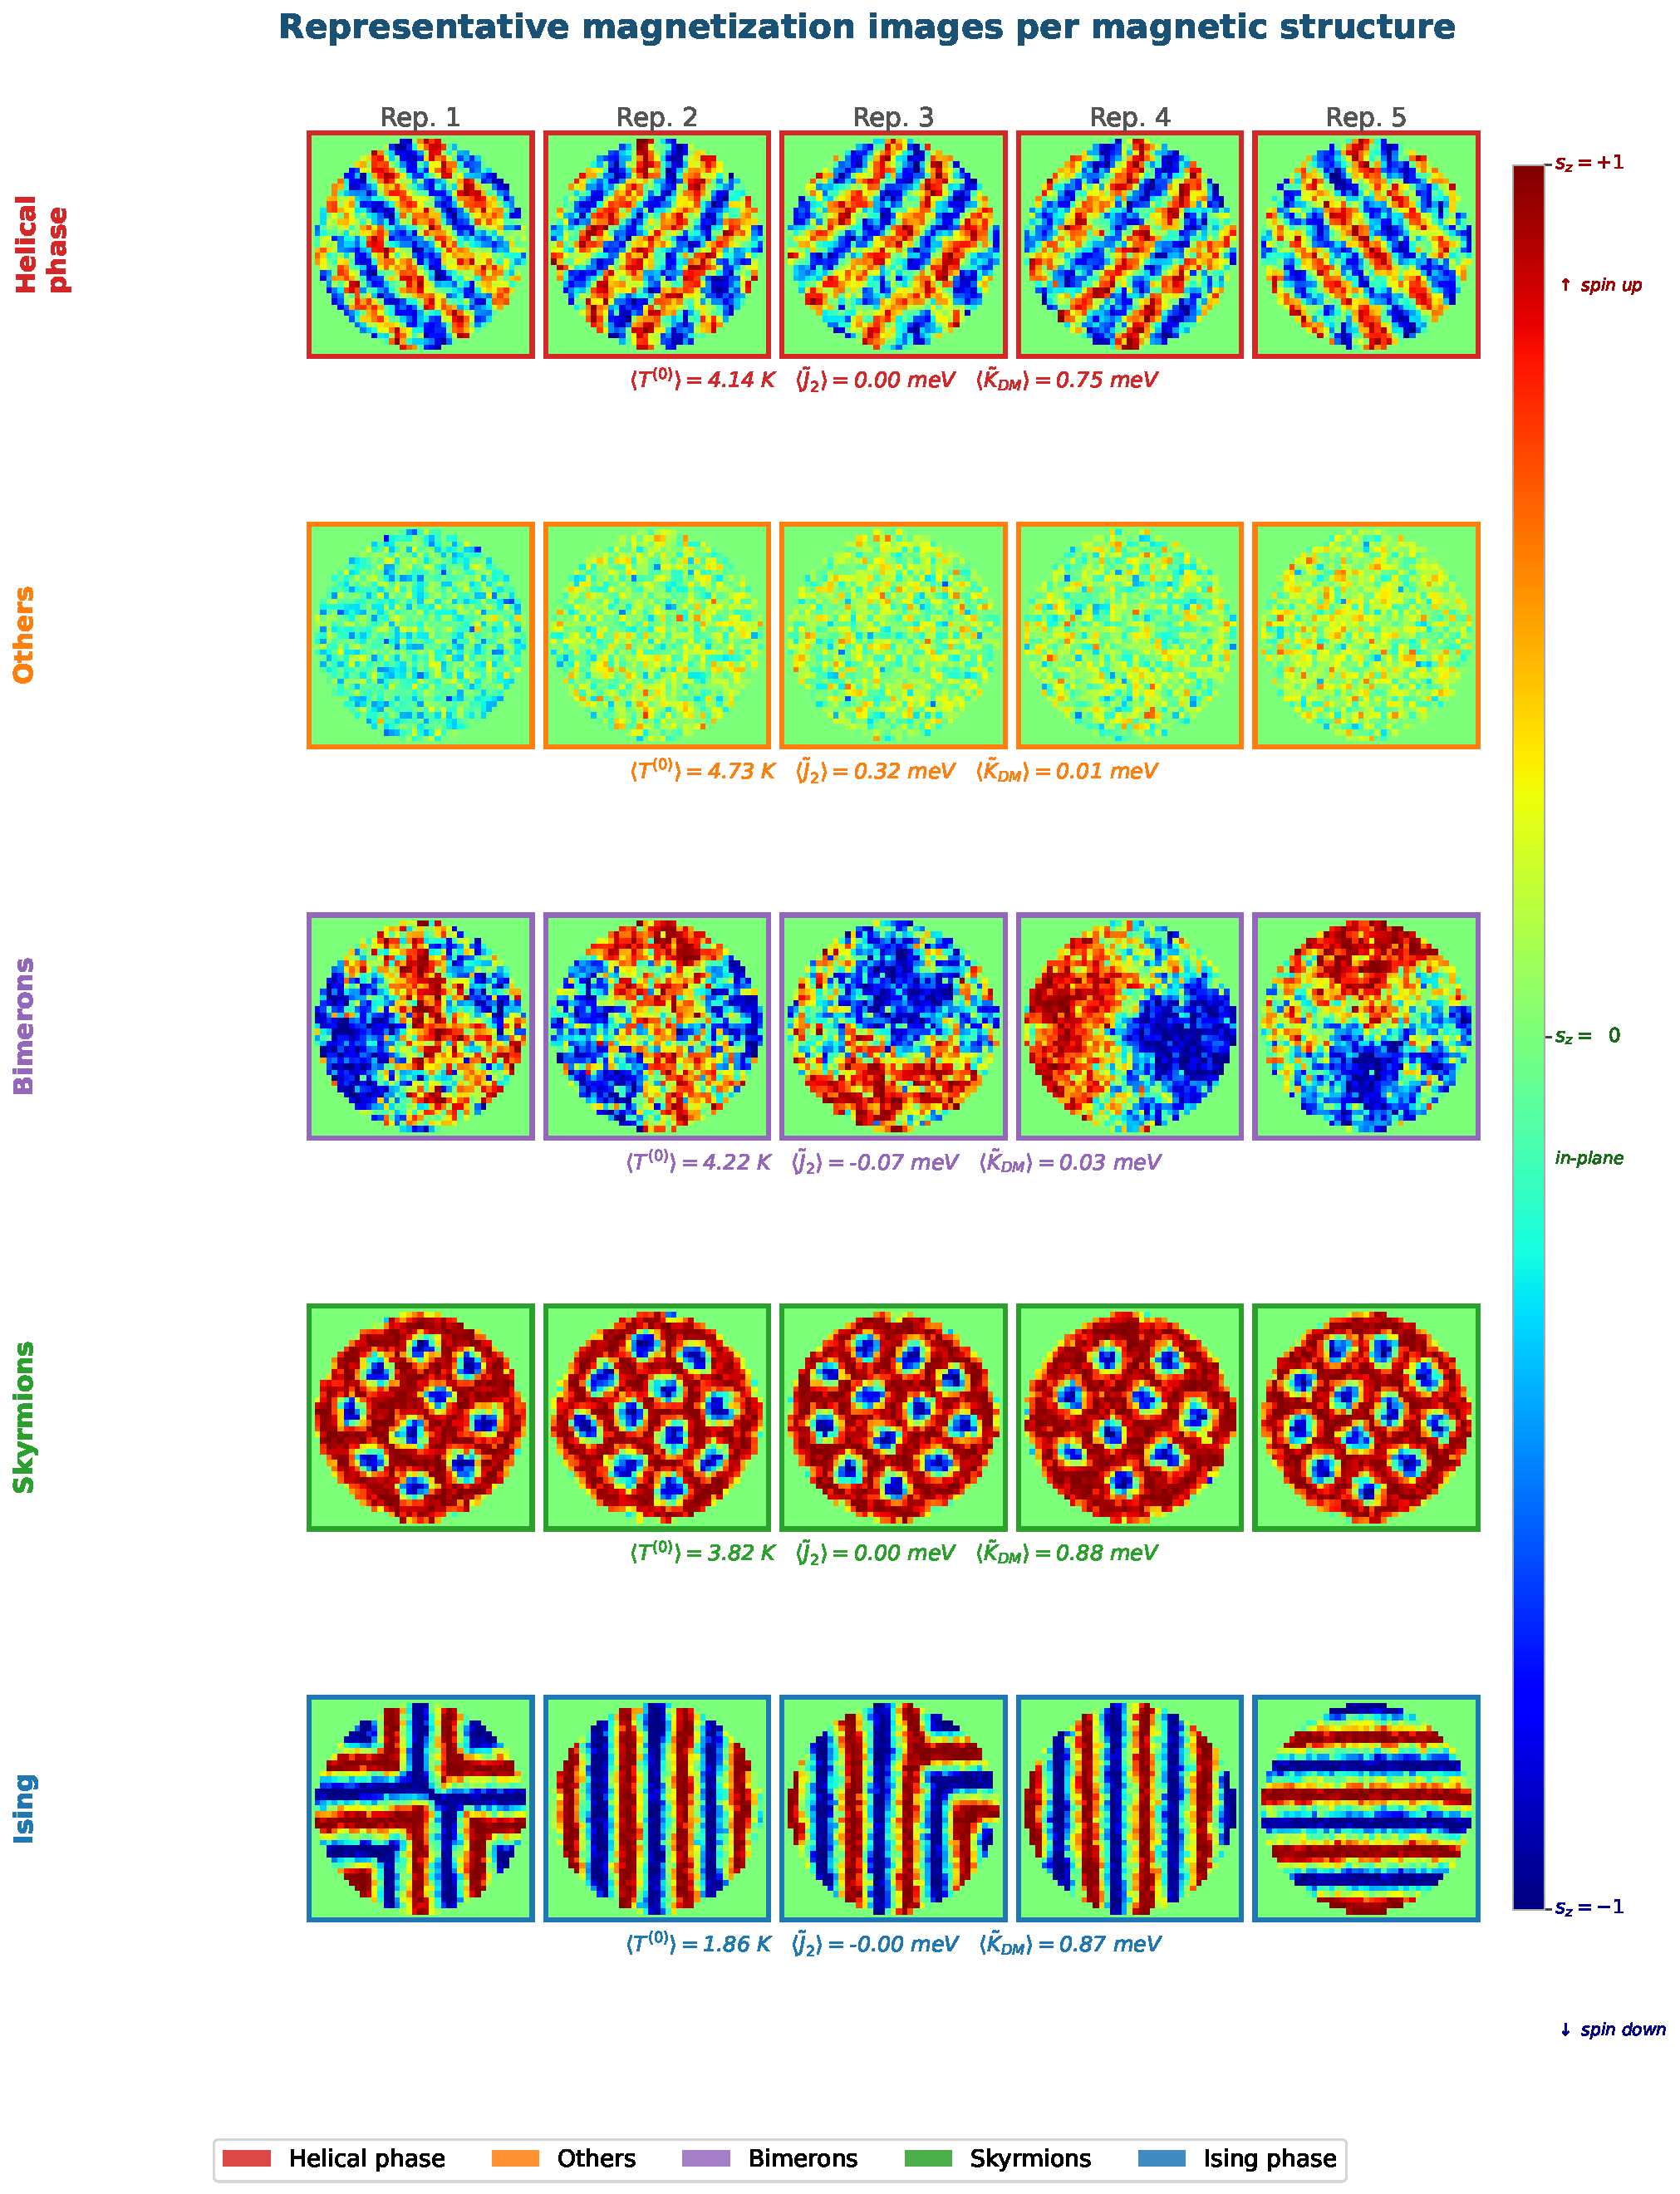
\includegraphics[width=0.5\linewidth]
    {structure_representatives}
    \caption{Representative magnetization images $\mathbf{X}_n$ 
    for each of the four magnetic phase categories identified 
    through clustering of the Vision Transformer latent space. 
    Each row displays five samples selected as the nearest 
    neighbors to the cluster centroid in the UMAP embedding. 
    Mean Hamiltonian parameters $\langle T^{(0)}\rangle$, 
    $\langle\tilde{J}_2\rangle$, and $\langle\tilde{K}_{DM}\rangle$ 
    are reported below each row. The Ferromagnetic phase displays 
    near-uniform $s_z$ distributions with minimal spatial 
    modulation. The Others category gathers thermally disordered, 
    transitional, and topologically mixed configurations that 
    lack a defining spatial signature and represent the most 
    structurally ambiguous samples in the dataset. The 
    Labyrinthine \& Conical phase exhibits spatially extended 
    stripe and labyrinthine domain patterns with clear chiral 
    winding. The Helical phase presents the most ordered and 
    spatially coherent helical stripe configurations in the 
    dataset, with consistent periodicity and chiral winding 
    direction across the entire nanodot.}
    \label{fig:structure_representatives}
\end{figure*}

The per-phase regression performance of the Vision Transformer,
evaluated on the 8,000 test samples used for the clustering
analysis, is summarized in Figures~\ref{fig:metrics_by_structure}
and~\ref{fig:mae_by_structure}. The results reveal a pronounced
heterogeneity in predictive accuracy across magnetic phases that
is physically consistent with the identifiability analysis
presented earlier in this section. The labyrinthine \& conical
and helical phases achieve the highest $R^2$ values and the
lowest MAE across all architectures, particularly for $T^{(0)}$
and $\tilde{K}_{DM}$, reflecting the fact that these ordered,
low-temperature configurations exhibit the most discriminative
and spatially coherent signatures in the $s_z$ projection.
Within these phases, the well-defined periodicity and chiral
winding of the magnetization texture provide unambiguous
observational constraints that allow the model to recover the
underlying Hamiltonian parameters with high fidelity.

In stark contrast, the \textit{others} category concentrates
the largest absolute errors across virtually all Hamiltonian
parameters, as evidenced by the dominant MAE values in
Figure~\ref{fig:mae_by_structure}. This result directly
confirms the physical interpretation advanced earlier: the
thermally disordered, transitional, and topologically mixed
configurations grouped in this category collapse into
structurally indistinguishable magnetization textures despite
corresponding to widely different parameter combinations,
making the inverse mapping fundamentally ill-posed within
this regime. The elevated MAE for $T^{(0)}$ in the
\textit{others} phase is particularly revealing, as it quantitatively isolates the
contribution of the high-temperature paramagnetic regime to
the global prediction error observed in the aggregated
analysis. Similarly, the Ferromagnetic phase exhibits
near-zero MAE for $\tilde{K}_{DM}$ and the exchange
constants, consistent with the near-constant values of
these parameters within this cluster and confirming that
the apparent low error in these cases reflects degeneracy
rather than genuine predictive capacity.

Within the ordered phases, the exchange constants
$\tilde{J}_2$, $\tilde{J}_3$, and $\tilde{J}_4$ yield
near-zero $R^2$ values for the Labyrinthine \& Conical
and Helical phases a direct consequence of the physical
constraint that these textures are generated exclusively
at $\tilde{J}_2 \approx 0$~meV, making the regression
target degenerate and the inverse mapping statistically
ill-posed for these parameters within these specific
structural regimes.

\begin{figure*}[t!]
    \centering
    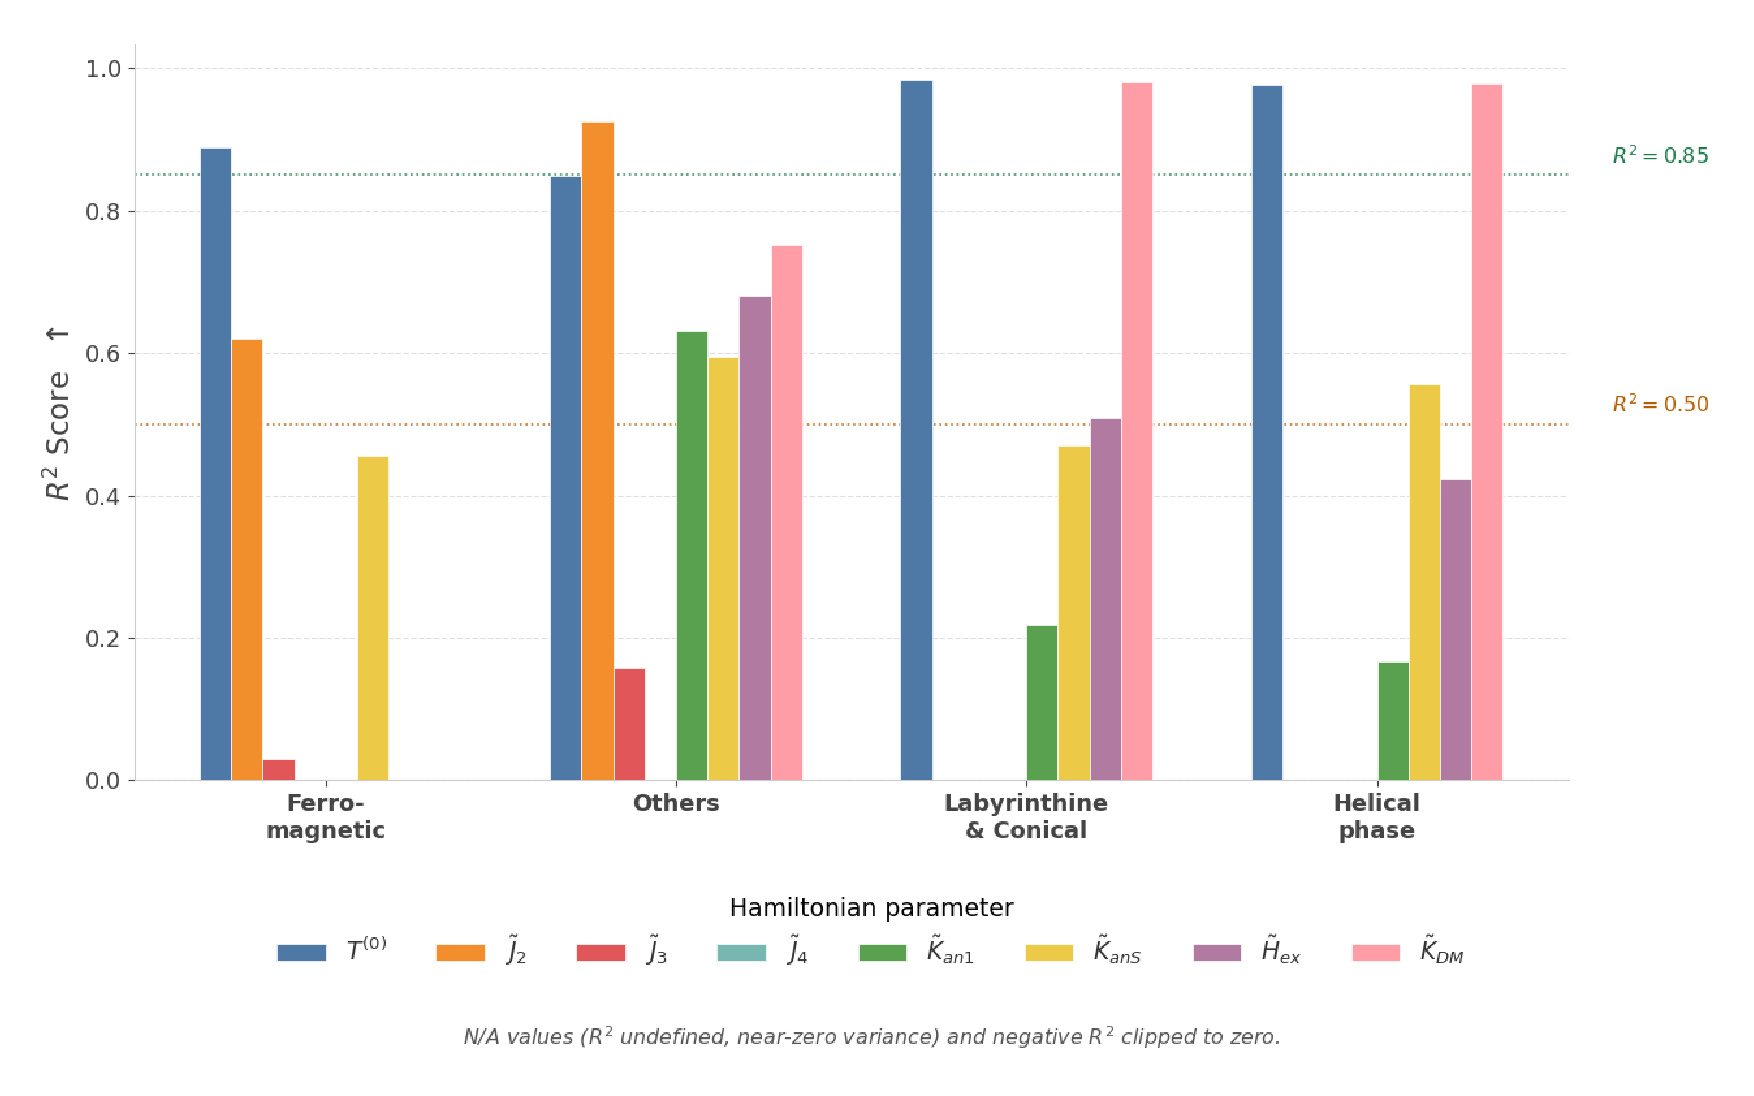
\includegraphics[width=0.8\linewidth, keepaspectratio]
    {R2_metrics_structure}
    \caption{Per-phase $R^2$ score of the Vision Transformer
    across all eight Hamiltonian parameters
    $\boldsymbol{\theta}$ for the four identified magnetic
    phase categories (test set, $N=8{,}000$). Each bar group
    corresponds to one magnetic phase and each bar to one
    target parameter. Dashed horizontal lines mark the
    identifiability thresholds at $R^2 = 0.85$ (high
    predictability) and $R^2 = 0.50$ (partial predictability).
    Negative $R^2$ values and near-zero variance cases (N/A)
    are clipped to zero. The Labyrinthine \& Conical and
    Helical phases achieve the highest accuracy for $T^{(0)}$
    and $\tilde{K}_{DM}$, while the Ferromagnetic phase
    exhibits the lowest identifiability due to the
    near-constant values of $\tilde{K}_{DM}$ and the exchange
    parameters within this topological regime.}
    \label{fig:metrics_by_structure}
\end{figure*}

\begin{figure*}[t!]
    \centering
    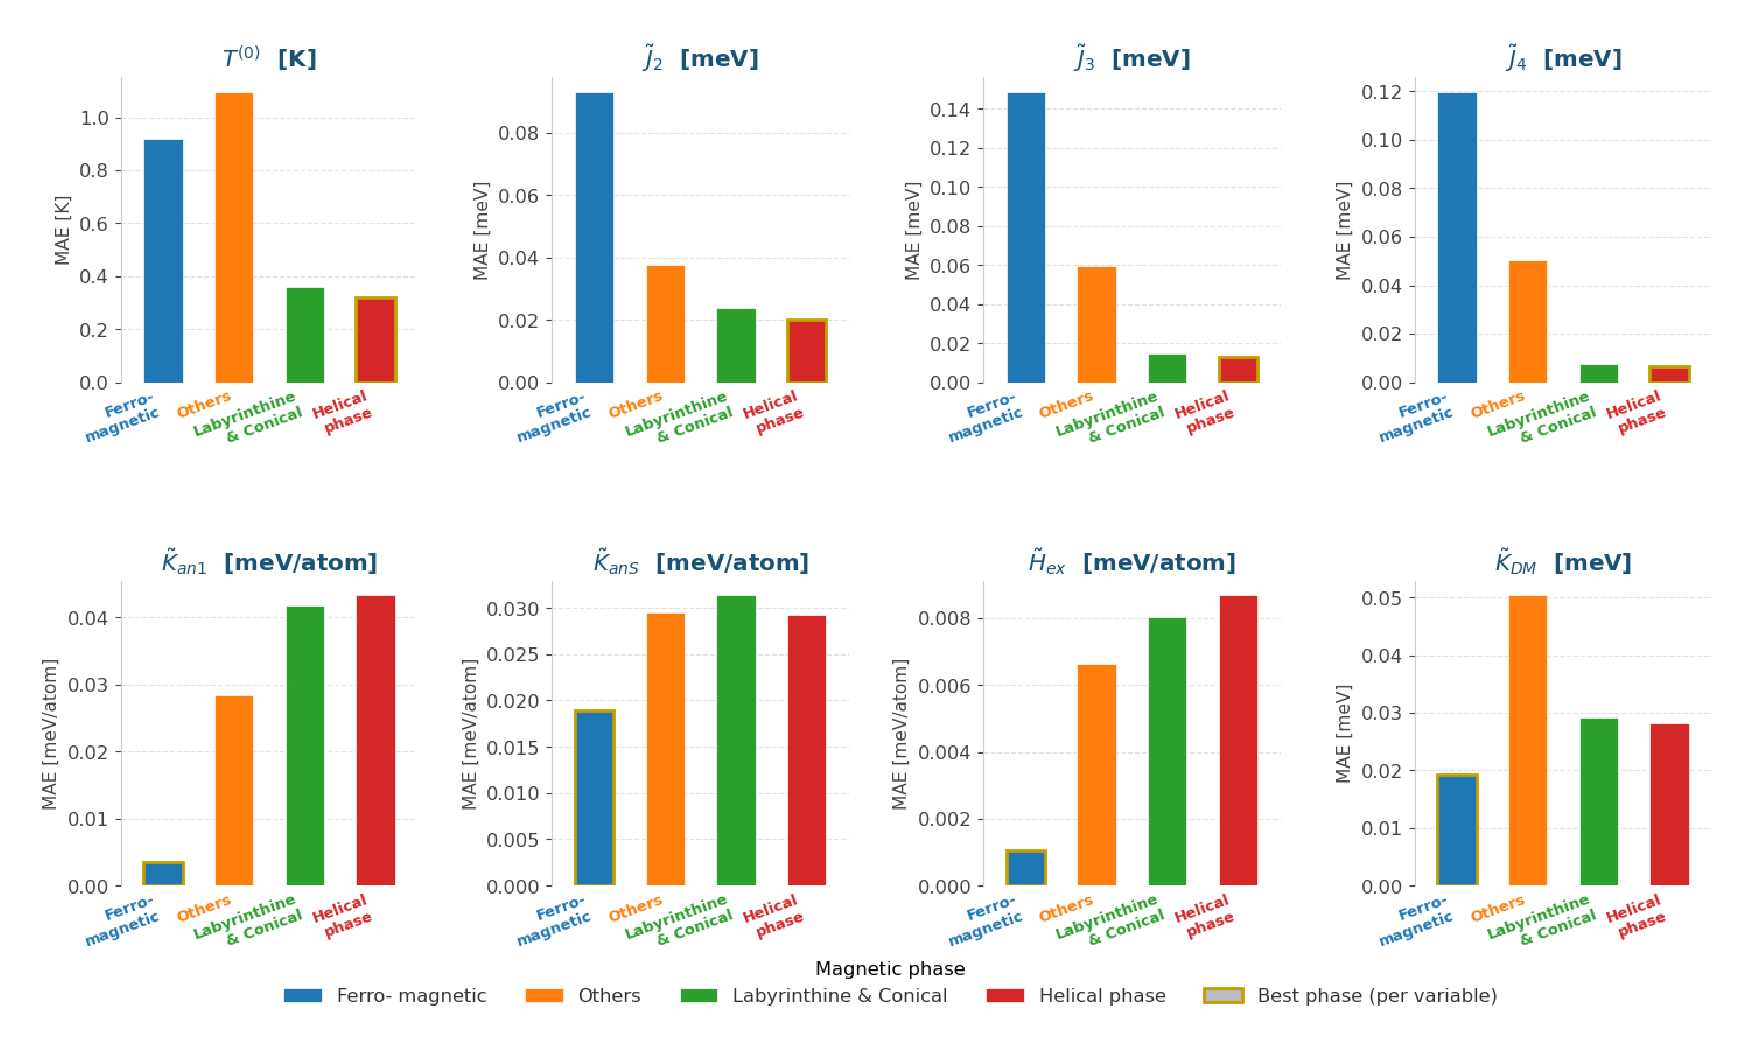
\includegraphics[width=\linewidth, keepaspectratio]
    {mae_structure}
    \caption{Per-phase Mean Absolute Error (MAE) of the Vision
    Transformer across all eight Hamiltonian parameters
    $\boldsymbol{\theta}$ for the four identified magnetic
    phase categories (test set, $N=8{,}000$), reported in the
    original physical units of each parameter after inverse
    Min-Max scaling. Each panel corresponds to one target
    parameter and shows one bar per magnetic phase. The
    \textit{others} category consistently concentrates the
    largest absolute errors across all parameters, confirming
    that the thermally disordered and transitional
    configurations within this group constitute the primary
    source of prediction error in the global regression
    analysis. Gold-bordered bars indicate the magnetic phase
gur    with the lowest MAE for each parameter.}
    \label{fig:mae_by_structure}
\end{figure*}

\subsection{RAMs-based Interpretability Results}
\label{sec:rams_results}

%\subsubsection{Spatial Interpretability via Xception}
To spatially trace the predictive behavior of the Xception
architecture across the identified magnetic phase categories,
RAMs were computed following the
CNN-based formulation introduced in
Section~\ref{sec:CNN_RAMs}. For each of the four magnetic
phases a single representative magnetization image
$\mathbf{X}_n$ was selected as the sample closest to the
centroid of the corresponding cluster group in the UMAP
latent space, maximizing the concentration of gradient
activations within the physical extent of the nanodot disk.
RAMs were computed for the three most identifiable
Hamiltonian parameters ($T^{(0)}$, $\tilde{J}_2$, and
$\tilde{K}_{DM}$) across eight strategically selected
convolutional layers of the Xception backbone, spanning the
full depth of the network:

\begin{itemize}
    \item[--] \texttt{block1\_conv2}: entry-level features
    at spatial resolution $112\times112$, capturing
    low-level pixel-scale magnetization gradients.
    \item[--] \texttt{block3\_sepconv2} and
    \texttt{block4\_sepconv2}: intermediate entry-flow
    layers at $56\times56$ and $28\times28$, encoding
    domain boundary frequencies and local spin-winding
    patterns.
    \item[--] \texttt{block6\_sepconv2} through
    \texttt{block12\_sepconv2}: middle-flow layers at
    $14\times14$, constituting the deepest repeated
    processing stage of Xception and encoding progressively
    more abstract topological representations of the
    magnetic texture.
    \item[--] \texttt{block13\_sepconv2}: exit-flow
    transition layer prior to global pooling, encoding
    high-level semantic representations of the global
    magnetic phase.
\end{itemize}

\paragraph{Selection of the precision factor $\gamma$.}
The precision factor $\gamma$ in the RAM objective
$\mathcal{O}_p = \exp\!\left(-\gamma\left(\theta_p -
\hat{\theta}_p\right)^2\right)$ governs the selectivity
of the gradient signal: small values render the objective
nearly constant regardless of prediction quality, producing
spatially uninformative maps, while excessively large values
collapse the gradient to zero for parameters with
non-negligible prediction error, yielding empty activation
maps. To select $\gamma$ in a principled and data-driven
manner, a sensitivity analysis was conducted by evaluating
the objective $\mathcal{O}_p$ at the empirical mean
prediction error $\bar{\varepsilon}_p =
\langle|\theta_p - \hat{\theta}_p|\rangle$ of each
Hamiltonian parameter on the test set, for values spanning
$\gamma \in \{0.1, 0.3, 0.5, 1, 2, 5, 10, 20, 50, 100\}$.

Figure~\ref{fig:gamma_selection} illustrates the resulting
sensitivity curves. The left panel shows the shape of the
Gaussian objective as a function of the prediction error
$\varepsilon$ for each candidate $\gamma$: values below
$\gamma = 1$ produce flat curves that activate uniformly
regardless of prediction quality, while values above
$\gamma = 20$ generate overly steep curves that suppress
the gradient for errors as small as $\varepsilon \approx
0.2$. The right panel evaluates $\mathcal{O}_p$ at the
empirical mean error of each parameter: all variables
maintain $\mathcal{O}_p > 0.5$ for $\gamma \leq 10$,
whereas for $\gamma \geq 20$ the parameters with larger
prediction errors --- specifically $T^{(0)}$ and
$\tilde{K}_{DM}$, whose mean errors reach $0.17$ and
$0.24$ respectively --- begin to approach the gradient
collapse threshold of $\mathcal{O}_p < 0.05$. The value
$\gamma = 10$ was therefore selected as the optimal
operating point: it is the most selective value that
simultaneously maintains a well-conditioned gradient
signal for all eight Hamiltonian parameters, ensuring
that the resulting RAMs are both spatially discriminative
and physically interpretable across the full
identifiability spectrum of the inverse problem.

\begin{figure*}[t!]
    \centering
    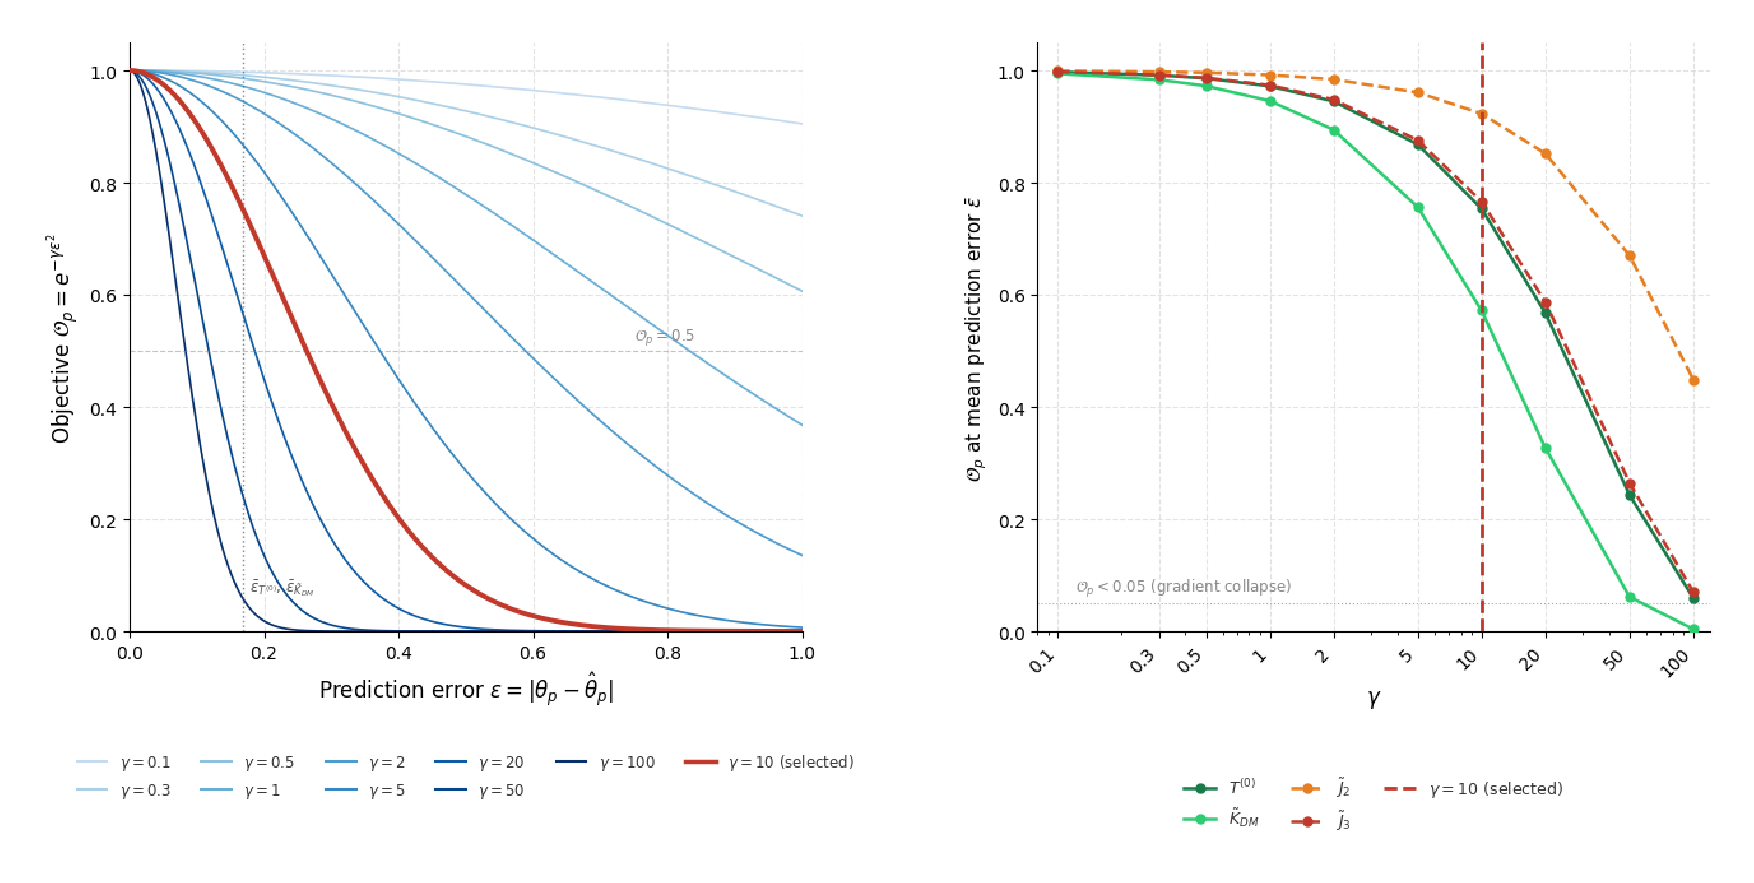
\includegraphics[width=\linewidth, keepaspectratio]
    {gamma_selection}
    \caption{Sensitivity analysis of the RAM precision
    factor $\gamma$. Left: shape of the Gaussian objective
    $\mathcal{O}_p = e^{-\gamma\varepsilon^2}$ as a
    function of the prediction error
    $\varepsilon = |\theta_p - \hat{\theta}_p|$ for
    $\gamma \in \{0.1, \dots, 100\}$; the selected value
    $\gamma = 10$ is highlighted in red. Vertical dotted
    lines indicate the empirical mean errors
    $\bar{\varepsilon}$ of $T^{(0)}$ and
    $\tilde{K}_{DM}$ on the test set. Right:
    $\mathcal{O}_p$ evaluated at $\bar{\varepsilon}_p$
    for each Hamiltonian parameter as a function of
    $\gamma$. The horizontal dotted line marks the
    gradient collapse threshold $\mathcal{O}_p = 0.05$.
    For $\gamma \leq 10$ all parameters maintain
    $\mathcal{O}_p > 0.5$; for $\gamma \geq 20$ the
    parameters with larger prediction errors begin to
    approach the collapse threshold. The value $\gamma =
    10$ is selected as the most selective operating point
    within the stable gradient regime.}
    \label{fig:gamma_selection}
\end{figure*}

To ensure that activation magnitudes remain physically
interpretable and spatially confined to the nanodot
geometry, each RAM was masked by a circular binary mask
aligned with the disk boundary prior to normalization.
The globally normalized RAMs
$\tilde{\mathcal{R}}_{\text{RAM}}^{(l,p)}$ were obtained
following Equation~\ref{eq:RAM_Global_Norm}, and the
spatial patterns were additionally visualized under local
per-cell normalization to reveal the gradient attribution
structure at each individual layer.

Figure~\ref{fig:rams_xception_unified} presents the
resulting RAM overlays for the two most topologically
structured phases --- Helical and Labyrinthine \& Conical
--- which were selected for visualization because their
highly ordered, low-temperature spin textures produce the
clearest and most physically interpretable gradient
attribution patterns among the four computed phases,
providing the strongest validation of the hierarchical
decoupling hypothesis. The spatial attribution patterns
reveal a physically consistent progression across network
depth. In the early entry-flow layers
(\texttt{block1\_conv2}, \texttt{block3\_sepconv2}),
activations are spatially dense and highly structured,
aligning with the fine-grained periodicity of the
magnetization texture --- particularly the stripe wavelength
and domain wall boundaries that carry the primary signature
of $\tilde{K}_{DM}$ and $T^{(0)}$. As depth increases
through the middle-flow layers (\texttt{block6} through
\texttt{block12}), activations progressively consolidate
into coarser, spatially localized hotspots that correspond
to topologically significant regions of the nanodot ---
notably the chiral domain wall junctions and large-scale
stripe boundaries characteristic of these two ordered
phases. In the terminal exit-flow layer
(\texttt{block13\_sepconv2}), activations become highly
concentrated in a small number of spatially compact regions,
suggesting that the network's final semantic representations
encode global topological stability rather than local
texture periodicity. This hierarchical progression is
consistent with the theoretical prediction of
Section~\ref{sec:Nor_RAMs}: early layers resolve the
short-range energetic competition between $\tilde{J}_1$
and $\tilde{K}_{DM}$, while deeper layers integrate these
local features into macro-scale thermodynamic
representations governed by $T^{(0)}$ and the
anisotropy constants.

\begin{figure*}[t!]
    \centering
    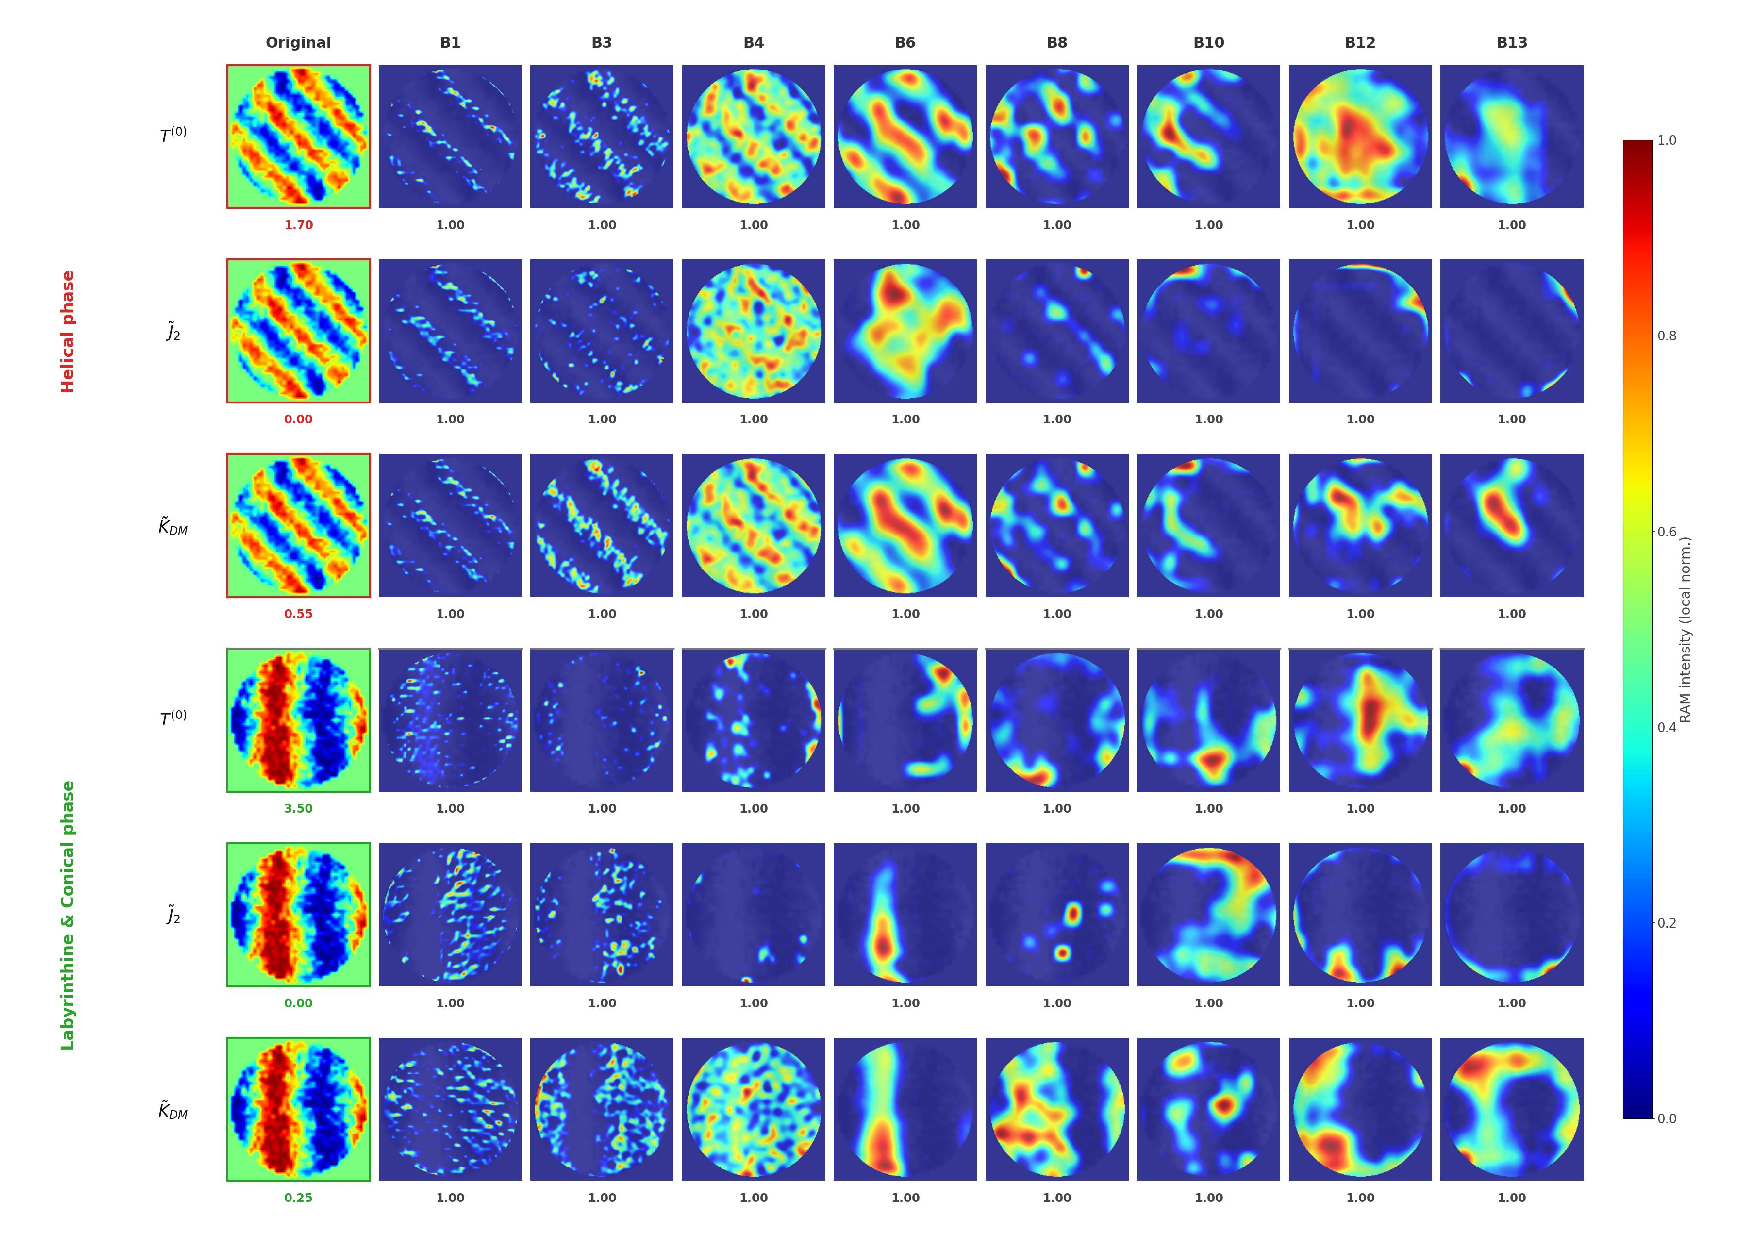
\includegraphics[width=0.7\linewidth]{rams_xception_unified}
    \caption{RAMs
    $\tilde{\mathcal{R}}_{\text{RAM}}^{(l,p)}$ for the
    Xception architecture, shown for the two most
    topologically structured magnetic phases --- Helical
    and Labyrinthine \& Conical --- selected as the most
    representative cases from the full four-phase RAM
    computation. Three Hamiltonian parameters
    $\{T^{(0)}, \tilde{J}_2, \tilde{K}_{DM}\}$ are
    shown. Each panel displays the RAM overlay (jet
    colormap) on the original $s_z$ magnetization image
    (grayscale), with local per-cell normalization to
    reveal spatial attribution patterns at each layer
    independently. Rows correspond to phase--parameter
    pairs; columns correspond to network layers from
    \texttt{block1} (entry, $112\times112$) to
    \texttt{block13} (exit, $14\times14$). The numerical
    score below each RAM cell reports the fraction of
    activation concentrated within the nanodot disk
    boundary, and the value below each original image
    reports the ground-truth parameter value for that
    representative sample. A physically consistent
    hierarchical decoupling is observed: early layers
    capture fine-grained domain periodicity while deeper
    layers consolidate activations into topologically
    significant spatial hotspots.}
    \label{fig:rams_xception_unified}
\end{figure*}

To quantify the relative importance of each network layer
and each Hamiltonian parameter in driving the gradient
response, Figure~\ref{fig:rams_xception_bars} presents
the mean maximum RAM activation per layer and variable,
averaged over $N=300$ randomly sampled test images per
magnetic phase. To enable meaningful cross-layer and
cross-parameter comparisons, the raw activation values
were standardized via a global z-score transform across
all layers and variables within each phase, and subsequently
mapped through a sigmoid function
$\sigma\!\left(\frac{x - \mu}{\sigma_x}\right) \in (0,1)$,
where $\mu$ and $\sigma_x$ denote the global mean and
standard deviation of the raw activations for each variable.
This normalization preserves the relative ordering of
activation magnitudes while compressing outliers and
centering the scale around $\sigma = 0.5$, such that
values above this threshold indicate above-average gradient
response for that parameter at that layer depth.

This statistical analysis confirms and extends the
qualitative observations from the spatial maps. Across
all four phases, the sigmoid-normalized activation profile
exhibits a non-monotonic behavior across depth, with
notable peaks at \texttt{block8\_sepconv2} and
\texttt{block13\_sepconv2}. The \texttt{block8} peak is
particularly pronounced for $\tilde{J}_3$ in the
\textit{Others} phase, suggesting that this middle-flow
layer has learned to specifically encode the subtle
energetic contributions of longer-range exchange
interactions in the heterogeneous and topologically mixed
configurations that characterize this category. The
\texttt{block13} peak, by contrast, is dominated by
$\tilde{J}_2$ and $T^{(0)}$ across all phases, consistent
with its role as a high-level semantic aggregator of the
dominant physical parameters. The anisotropy constants
$\tilde{K}_{an1}$ and $\tilde{K}_{anS}$ and the external
field $\tilde{H}_{ex}$ systematically exhibit the lowest
sigmoid activations across all layers and phases ---
consistently below $\sigma = 0.5$ --- corroborating their
limited identifiability established in
Section~\ref{sec:dl_results} and confirming that the
Xception backbone has not learned spatially distinctive
features for these parameters, a result fully consistent
with their physical coupling to the in-plane spin
components $s_x$ and $s_y$ that are not observable in
the $s_z$ projection.

\begin{figure*}[t!]
    \centering
    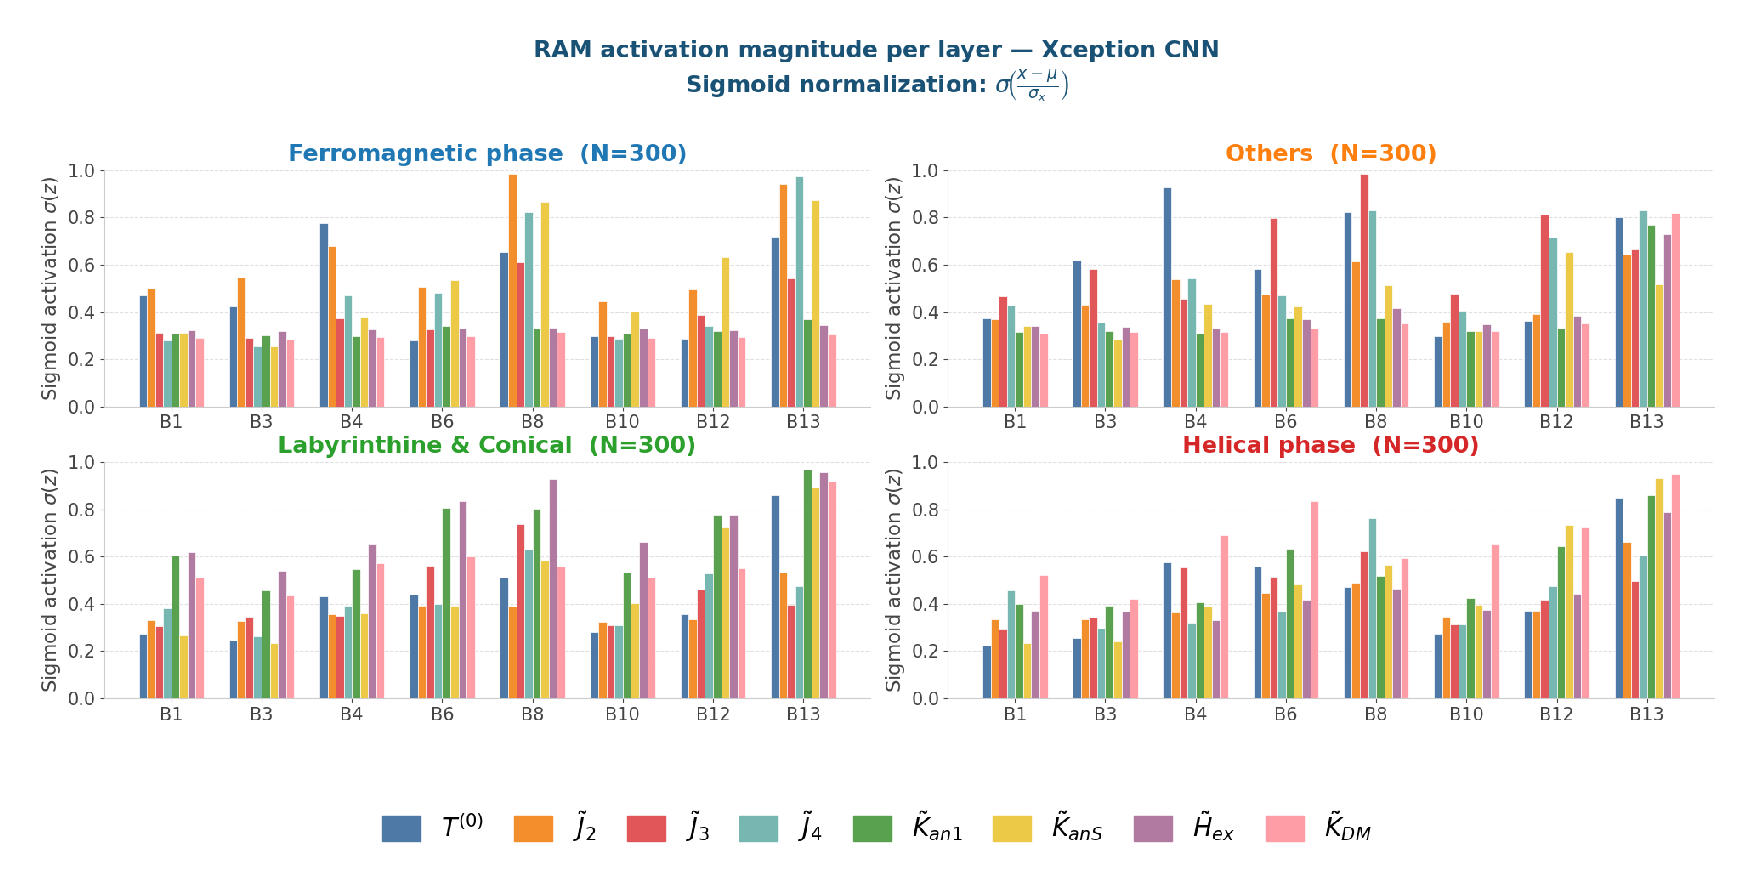
\includegraphics[width=\linewidth]
    {rams_xception_bars}
    \caption{Mean maximum RAM activation per network
    layer and Hamiltonian parameter $\boldsymbol{\theta}$,
    averaged over $N=300$ test samples per magnetic phase
    (Xception CNN). Activations are reported after
    sigmoid normalization
    $\sigma\!\left(\frac{x-\mu}{\sigma_x}\right)$
    applied globally per variable, where values above
    $\sigma=0.5$ indicate above-average gradient response.
    Each color corresponds to a distinct parameter
    following the nomenclature of
    Table~\ref{tab:param_ranges}. Activation is measured
    exclusively within the nanodot disk boundary (masked
    RAM). The non-monotonic depth profile with peaks at
    \texttt{block8} and \texttt{block13} reveals that the
    network resolves short-range exchange and DMI features
    in intermediate layers while aggregating global
    thermodynamic representations in the terminal
    exit-flow layer. Parameters with low identifiability
    ($\tilde{K}_{an1}$, $\tilde{K}_{anS}$,
    $\tilde{H}_{ex}$) consistently exhibit minimal
    sigmoid activation across all layers and phases,
    confirming the partial observability limitations
    identified in the regression analysis.}
    \label{fig:rams_xception_bars}
\end{figure*}

%\subsubsection{Spatial Interpretability via Vision Transformer}

An analogous interpretability analysis was conducted for
the Vision Transformer using the ViT-based RAM formulation
introduced in Section~\ref{sec:ViT_RAMs}. In contrast
to Xception, which operates through a hierarchy of
convolutional feature maps at varying spatial resolutions,
the Vision Transformer processes the input magnetization
image $\mathbf{X}_n$ as a sequence of $N_r = 196$
non-overlapping $16\times16$ patches, producing a
pseudo-feature map $\mathbf{A}_{\text{ViT}} \in
\mathbb{R}^{14\times14\times768}$ upon token reshaping.
Because the ViT architecture does not possess intermediate
spatial hierarchies analogous to convolutional layers, the
RAM analysis collapses to a single spatial attribution map
per parameter, derived from the gradient of the
error-decay objective $\mathcal{O}_p$ with respect to the
spatial token embeddings $\mathbf{Z}_s$ at the output of
the terminal encoder block.

Figure~\ref{fig:rams_vit_compact} presents the ViT RAM
overlays for all four magnetic phases across the three
most identifiable parameters. The spatial attribution
patterns produced by the Vision Transformer are
qualitatively distinct from those of Xception in two
physically meaningful ways. First, the ViT RAMs exhibit
smoother, patch-level spatial resolution consistent with
the $14\times14$ token grid, capturing activation patterns
at the scale of the magnetic domain wavelength rather
than at the pixel level. This coarser but globally
coherent attribution is a direct consequence of the
self-attention mechanism, which explicitly correlates
distant patches and therefore encodes long-range spin
correlations that are physically relevant for parameters
governing global magnetic order such as $T^{(0)}$ and
$\tilde{K}_{DM}$. Second, the ViT RAMs display a
stronger phase-specificity: for the Helical and
Labyrinthine \& Conical phases, activations concentrate
along the chiral stripe boundaries and domain wall
junctions --- precisely the spatial features that encode
the DMI-driven winding angle and the exchange-controlled
domain spacing. Notably, the \textit{Others} phase
representative exhibits the highest annealing temperature
in the dataset ($T^{(0)} = 17.00$~K), placing it well
above the effective Curie temperature and producing a
fully disordered paramagnetic texture; accordingly, the
corresponding RAMs are spatially diffuse and structurally
uninformative, reflecting the fundamental degeneracy of
this regime. For the Ferromagnetic phase, the activations
for $\tilde{K}_{DM}$ are notably sparse and peripheral,
consistent with the near-zero DMI value ($\tilde{K}_{DM}
= 0.00$~meV) of the representative sample and the
model's inability to identify physically meaningful DMI
features in the absence of chiral spin winding.

\begin{figure*}[t!]
    \centering
    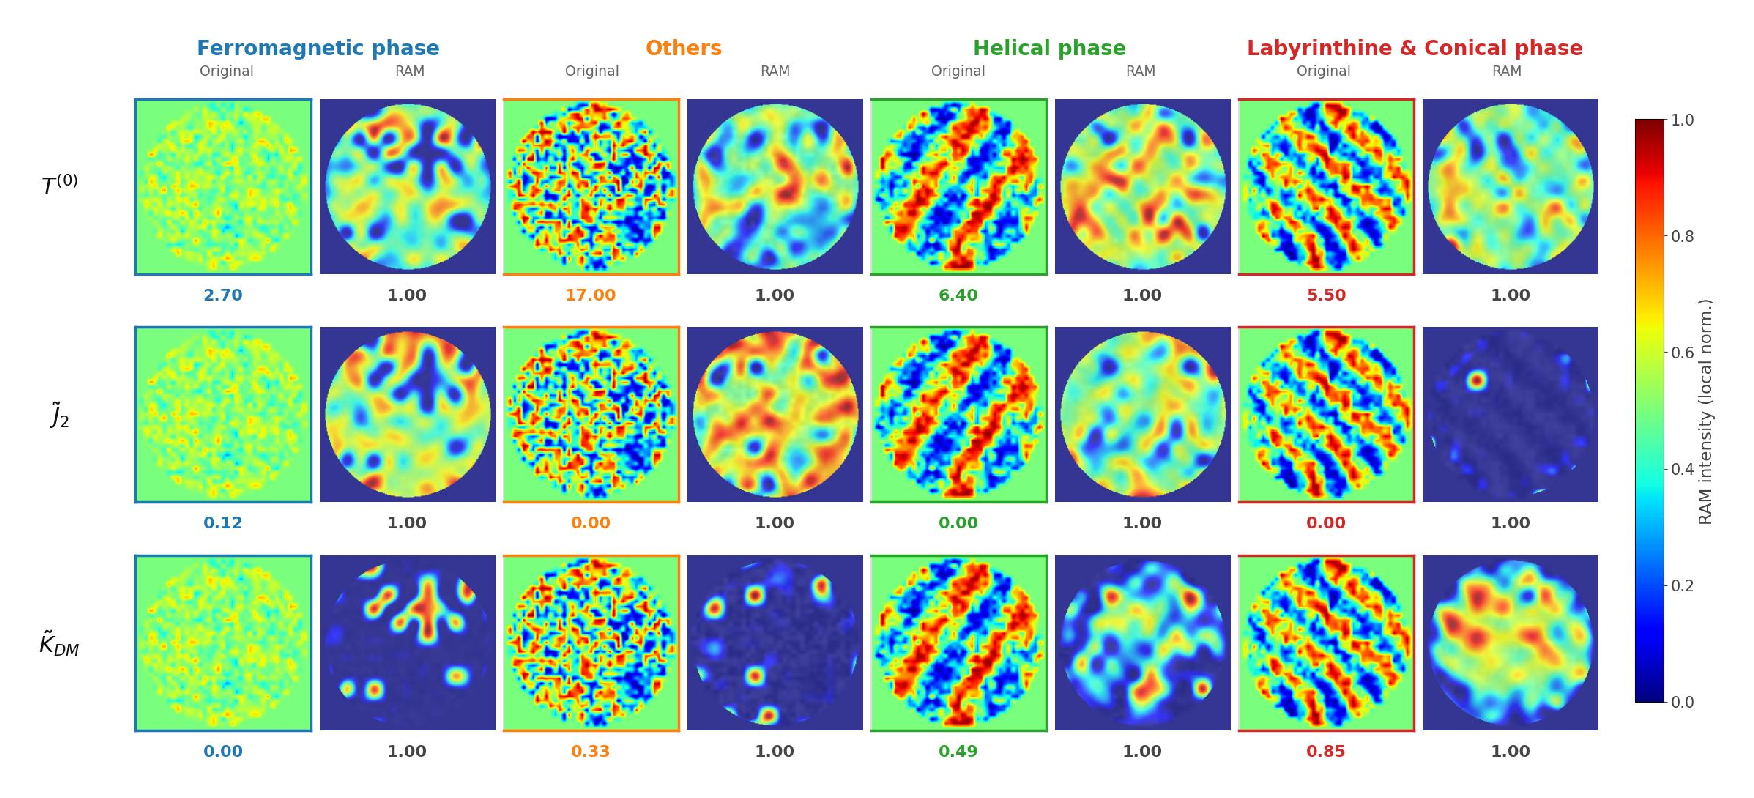
\includegraphics[width=\linewidth]
    {rams_vit_compact}
    \caption{RAMs
    $\tilde{\mathcal{R}}_{\text{RAM}}^{(p)}$ for the
    Vision Transformer across the four identified magnetic
    phases and three Hamiltonian parameters
    $\{T^{(0)}, \tilde{J}_2, \tilde{K}_{DM}\}$. Each
    panel pair displays the original $s_z$ magnetization
    image (left) and the corresponding RAM overlay on
    grayscale (right), derived from gradients of the
    error-decay objective $\mathcal{O}_p$ with respect
    to the reshaped spatial token embeddings
    $\mathbf{A}_{\text{ViT}} \in
    \mathbb{R}^{14\times14\times768}$. Score values
    report the fraction of activation within the nanodot
    boundary. The ground-truth parameter values reported
    below each original image confirm the physical
    regime of each representative: $\tilde{K}_{DM} =
    0.00$~meV in the Ferromagnetic phase, $T^{(0)} =
    17.00$~K in the \textit{Others} phase reflecting
    a fully disordered paramagnetic configuration, and
    $\tilde{J}_2 = 0.00$~meV in both the Helical and
    Labyrinthine \& Conical phases consistent with the
    energetic dominance of $\tilde{K}_{DM}$ in these
    chiral regimes. The ViT RAMs exhibit smooth,
    patch-scale spatial attribution with strong
    phase-specificity, concentrating on chiral domain
    walls and stripe boundaries in the ordered phases
    while producing spatially diffuse activations for
    the thermally degenerate \textit{Others} phase.}
    \label{fig:rams_vit_compact}
\end{figure*}

Figure~\ref{fig:rams_vit_bars} quantifies the mean
maximum RAM activation per Hamiltonian parameter
across all four magnetic phases for the Vision
Transformer. Unlike the layer-resolved profile of
Xception, the ViT activation spectrum reflects the
integrated gradient response of the full token
embedding space $\mathbf{Z}_s \in
\mathbb{R}^{196\times768}$ for each parameter, with
no layer hierarchy to resolve since the backbone
produces a single sequence of spatial tokens.
To enable meaningful cross-parameter and cross-phase
comparisons, the raw activation values were
standardized via a global z-score transform and
subsequently mapped through a sigmoid function
$\sigma\!\left(\frac{x - \mu}{\sigma_x}\right)
\in (0,1)$, where $\mu$ and $\sigma_x$ denote the
global mean and standard deviation of the raw
activations for each variable across all phases.
Values above $\sigma = 0.5$ indicate above-average
gradient response for that parameter, providing a
physically interpretable threshold for assessing
relative parameter identifiability within the ViT
token space.

The results reveal a physically consistent and
phase-specific hierarchy of parameter identifiability.
In the \textit{Ferromagnetic} phase, $T^{(0)}$,
$\tilde{J}_2$, and $\tilde{J}_3$ dominate the
activation spectrum with sigmoid values well above
$\sigma = 0.5$, reflecting the primacy of thermal and
exchange-driven ordering as the primary discriminative
features for this topologically simple configuration.
The \textit{Others} phase exhibits a more uniform and
globally suppressed activation profile, consistent with
the heterogeneous and thermally disordered nature of
the configurations in this category, where no single
parameter produces a spatially distinctive and
consistent gradient signal across the ensemble of
300 samples. In the \textit{Labyrinthine \& Conical}
phase, the activation spectrum shifts markedly toward
the higher-order exchange constant $\tilde{J}_4$,
the anisotropy parameters $\tilde{K}_{an1}$ and
$\tilde{K}_{anS}$, the external field $\tilde{H}_{ex}$,
and the DMI strength $\tilde{K}_{DM}$, all exhibiting
sigmoid activations above $\sigma = 0.5$. This result
suggests that the ViT has learned to resolve the
energetic competition between chiral and anisotropic
interactions that stabilizes the labyrinthine domain
structure at low temperatures. Finally, in the
\textit{Helical} phase, $\tilde{K}_{anS}$,
$\tilde{H}_{ex}$, and $\tilde{K}_{DM}$ clearly
dominate the activation spectrum, consistent with
the strong chiral winding and surface-symmetry-breaking
effects that produce the spatially coherent helical
stripe patterns characteristic of this phase.
Across all phases, $\tilde{J}_3$ and $\tilde{J}_4$
maintain systematically low activations --- with the
exception of $\tilde{J}_4$ in the Labyrinthine \&
Conical phase --- confirming that the ViT's global
attention mechanism is generally unable to isolate
spatially distinctive features for these energetically
subordinate higher-order exchange constants. Taken
together, the ViT RAM activation spectra provide a
direct, architecture-agnostic validation of the
identifiability hierarchy established through the
regression analysis, demonstrating that the model's
internal representations are physically grounded
rather than statistically arbitrary.

\begin{figure*}[t!]
    \centering
    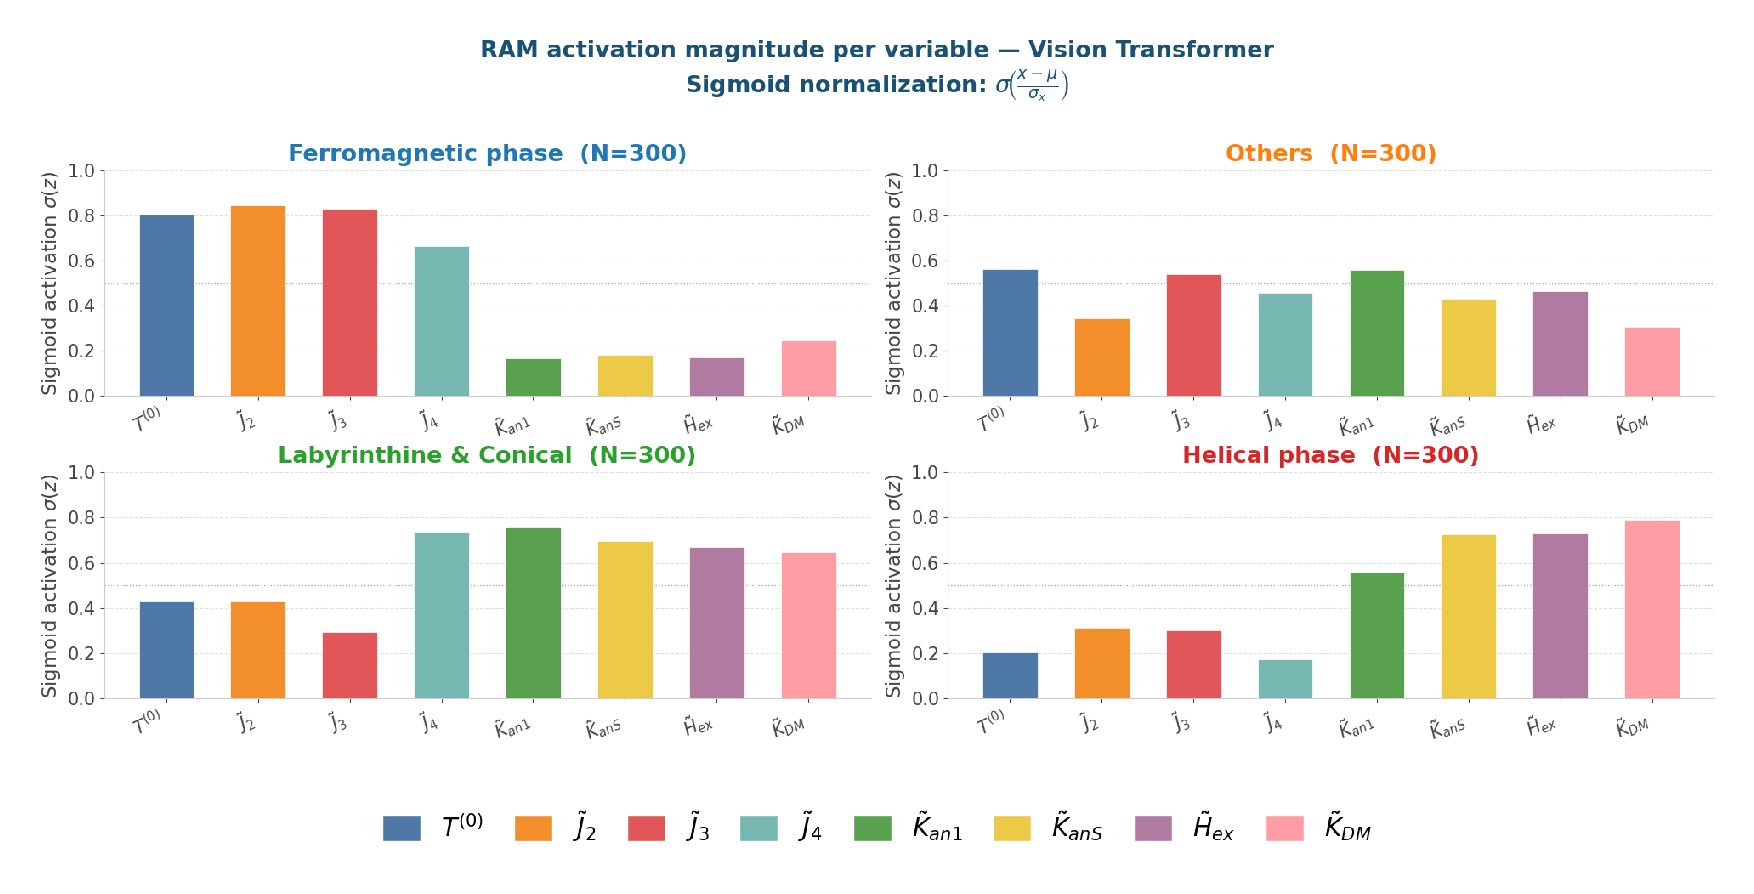
\includegraphics[width=\linewidth]
    {rams_vit_bars}
    \caption{Mean maximum RAM activation per Hamiltonian
    parameter $\boldsymbol{\theta}$, averaged over
    $N=300$ test samples per magnetic phase (Vision
    Transformer). Activations are reported after
    sigmoid normalization
    $\sigma\!\left(\frac{x-\mu}{\sigma_x}\right)$
    applied globally per variable across all phases,
    where values above $\sigma=0.5$ indicate
    above-average gradient response. Activation is
    measured within the nanodot disk boundary from
    gradients of $\mathcal{O}_p$ with respect to the
    reshaped spatial token embeddings
    $\mathbf{A}_{\mathrm{ViT}} \in
    \mathbb{R}^{14\times14\times768}$
    (Equation~\ref{eq:ViT_Reshape}). Each bar color
    corresponds to a distinct parameter following the
    nomenclature of Table~\ref{tab:param_ranges}.
    The Ferromagnetic phase is dominated by $T^{(0)}$,
    $\tilde{J}_2$, and $\tilde{J}_3$; the
    \textit{Others} phase shows a uniformly suppressed
    spectrum reflecting its thermally degenerate
    character; the Labyrinthine \& Conical phase
    activates strongly on $\tilde{J}_4$,
    $\tilde{K}_{an1}$, $\tilde{K}_{anS}$,
    $\tilde{H}_{ex}$, and $\tilde{K}_{DM}$; and the
    Helical phase is governed by $\tilde{K}_{anS}$,
    $\tilde{H}_{ex}$, and $\tilde{K}_{DM}$,
    corroborating the identifiability analysis of
    Section~\ref{sec:dl_results}.}
    \label{fig:rams_vit_bars}
\end{figure*}

%\subsubsection{Comparative Analysis and Physical Interpretation}

Comparing the RAM-based interpretability results 
across Xception and the Vision Transformer reveals 
two complementary and physically consistent 
perspectives on how deep learning architectures 
resolve the inverse Hamiltonian estimation problem. 
Xception operates through a hierarchical spatial 
decomposition: early convolutional layers capture 
fine-grained domain periodicity and boundary 
chirality at high spatial resolution, while deeper 
middle-flow and exit-flow layers progressively 
consolidate these local features into coarser, 
topologically meaningful representations of the 
global magnetic phase. This hierarchical decoupling 
mirrors the multi-scale energetic competition of the 
extended Heisenberg Hamiltonian, where short-range 
exchange interactions ($\tilde{J}_1$, $\tilde{J}_2$) 
set the local domain scale while long-range DMI 
and thermodynamic effects ($\tilde{K}_{DM}$, 
$T^{(0)}$) govern global phase stability. The Vision 
Transformer, by contrast, resolves the same physical 
information through a single-scale, globally coherent 
patch-level attribution, leveraging multi-head 
self-attention to explicitly correlate distant spin 
textures across the nanodot. This architectural 
difference explains why the Vision Transformer 
achieves marginally superior overall regression 
performance --- its global receptive field more 
efficiently captures the long-range topological 
coherence that distinguishes the identifiable 
parameters $T^{(0)}$ and $\tilde{K}_{DM}$ from 
the degenerate ones. In both architectures, the 
RAM analysis isolates the same set of physically 
meaningful spatial features as the primary drivers 
of accurate regression: chiral domain wall 
boundaries, stripe periodicity, and skyrmion-like 
core structures. Conversely, both architectures 
fail to produce spatially concentrated activations 
for $\tilde{K}_{an1}$, $\tilde{K}_{anS}$, and 
$\tilde{H}_{ex}$, confirming that the limited 
identifiability of these parameters is not a 
consequence of insufficient model capacity but of 
the fundamental physical constraints of the inverse 
problem --- specifically, the partial observability 
of the anisotropy signal in the $s_z$ projection 
and the confounding of the Zeeman field with 
thermal disorder in the two-dimensional 
magnetization image.



\subsection{Comparative Analysis of Computational 
Inference Times}
\label{sec:inference_times}

To comprehensively characterize the practical deployment 
viability of the proposed inverse Hamiltonian estimation 
framework, a systematic computational cost analysis was 
conducted across all four evaluated architectures, 
encompassing both the training phase and the inference 
regime. All experiments were executed on an NVIDIA H100 
GPU (Google Colab Pro) with 97~GB of VRAM, using a unified
training protocol of batch size $B=512$ over a maximum of 
100 epochs with 299 gradient steps per epoch, subject to 
early stopping with patience of 8 epochs on the validation 
loss.

%\subsubsection{Training Computational Cost}

Figure~\ref{fig:training_times} presents the wall-clock 
training time per epoch and the per-step gradient update 
time for each architecture in the stable warm-start regime 
(epochs 2 onward, excluding the first epoch which incurs 
additional compilation and data-loading overhead). The 
results reveal a clear trade-off between model capacity 
and training efficiency. ResNet50 achieves the fastest 
training throughput at 65~s/epoch (217~ms/step), followed 
by DenseNet121 at 79~s/epoch (265~ms/step) and Xception 
at 103~s/epoch (343~ms/step). The Vision Transformer 
incurs the highest training cost at 167~s/epoch 
(558~ms/step) --- a factor of $2.6\times$ slower per 
epoch than ResNet50 and $1.6\times$ slower than Xception.

This elevated training cost of the Vision Transformer 
is a direct consequence of its architectural complexity: 
with 85.8~million trainable parameters --- $4.1\times$ 
more than Xception (20.8M), $12.3\times$ more than 
DenseNet121 (6.96M), and $16.7\times$ more than 
ResNet50 (25.6M) --- the self-attention mechanism 
requires substantially more floating-point operations per 
gradient step than the depthwise separable convolutions 
of the CNN baselines. Despite this overhead, the Vision 
Transformer's superior regression performance 
established in Section~\ref{sec:dl_results} demonstrates 
that this additional computational investment during 
training is justified by the quality of the learned 
Hamiltonian representations. The effective number of 
training epochs until early stopping convergence further 
modulates the total training wall-clock time: the Vision 
Transformer converged at epoch 68 while Xception 
converged at epoch 48, resulting in total training 
times of approximately 3.2~hours and 1.4~hours 
respectively.

\begin{figure*}[t!]
    \centering
    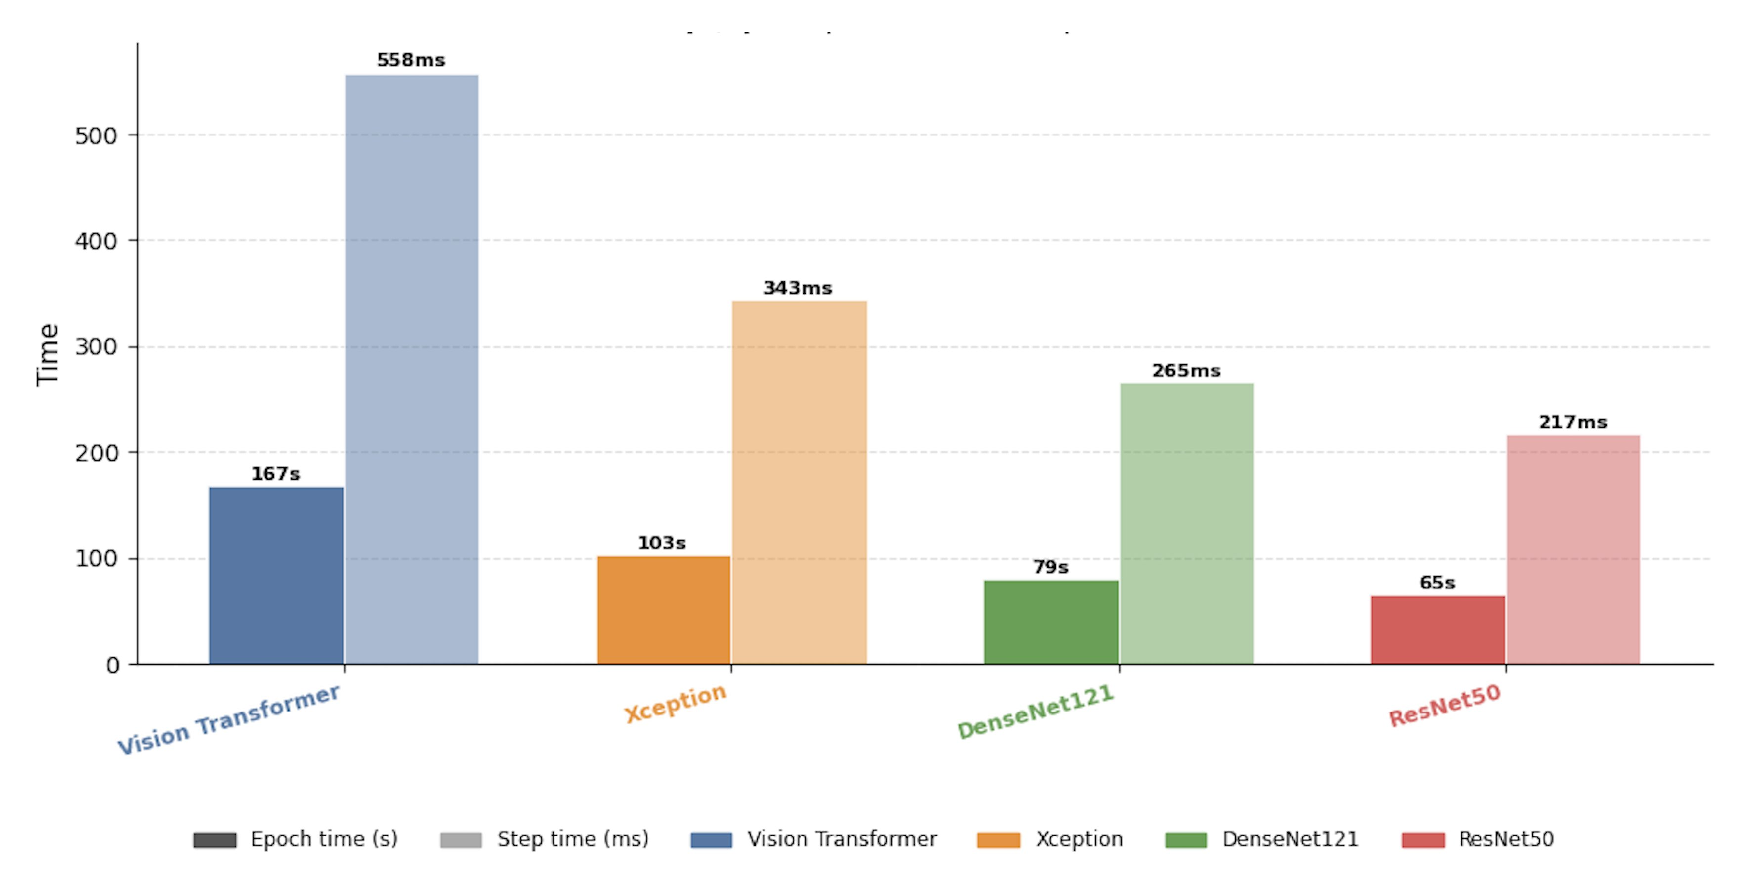
\includegraphics[width=0.9\linewidth]
    {training_times}
    \caption{Training computational cost comparison 
    across the four regression architectures on an 
    NVIDIA H100 GPU (Google Colab Pro). 
    \textbf{(a)} Wall-clock time per epoch in the 
    stable warm-start regime. 
    \textbf{(b)} Per-step gradient update time 
    (299 steps/epoch, batch size $B=512$). The Vision 
    Transformer incurs the highest training cost 
    (167~s/epoch, 558~ms/step) due to its 
    85.8M-parameter self-attention architecture, while 
    ResNet50 achieves the fastest throughput 
    (65~s/epoch, 217~ms/step). The training cost 
    hierarchy directly reflects the architectural 
    complexity of each model.}
    \label{fig:training_times}
\end{figure*}

%\subsubsection{Inference Latency Analysis}

Figure~\ref{fig:inference_times} presents the inference 
latency measurements for all four architectures across 
four batch sizes ($B \in \{1, 8, 32, 128\}$), 
quantifying both the total batch processing time and the 
per-image throughput. Inference times are reported as 
mean $\pm$ standard deviation over $N=10$ forward passes 
with 3 warmup passes excluded to eliminate GPU 
initialization effects.

The single-sample inference regime ($B=1$) is the most 
relevant scenario for real-time physical characterization 
applications, where individual magnetization images are 
acquired sequentially and must be processed 
independently. In this regime, Xception achieves the 
lowest latency at $127.71 \pm 1.46$~ms/image, followed 
by the Vision Transformer at $188.89 \pm 4.09$~ms/image. 
DenseNet121 exhibits the highest single-image latency at 
$459.77 \pm 7.22$~ms/image --- substantially slower than 
both architectures with significantly more parameters --- 
a consequence of its densely connected skip connections 
that generate large intermediate feature tensors and 
cause memory bandwidth saturation on single-image 
workloads.

In the batch inference regime ($B=128$), the per-image 
latency collapses dramatically across all architectures 
due to GPU parallelism. Xception again achieves the 
best throughput at $1.47 \pm 0.007$~ms/image, followed 
by the Vision Transformer at $1.92 \pm 0.033$~ms/image. 
This represents a $86.8\times$ speedup for Xception 
and a $98.4\times$ speedup for the Vision Transformer 
relative to their respective single-image latencies, 
demonstrating that both architectures are highly amenable 
to parallel batch processing in large-scale 
characterization pipelines. The throughput gap between 
Xception and the Vision Transformer narrows 
substantially at $B=128$ ($1.47$ vs. $1.92$~ms/image, 
a factor of only $1.31\times$), suggesting that the 
Vision Transformer's self-attention parallelism becomes 
increasingly competitive with convolutional processing 
at larger batch sizes.

\begin{figure*}[t!]
    \centering
    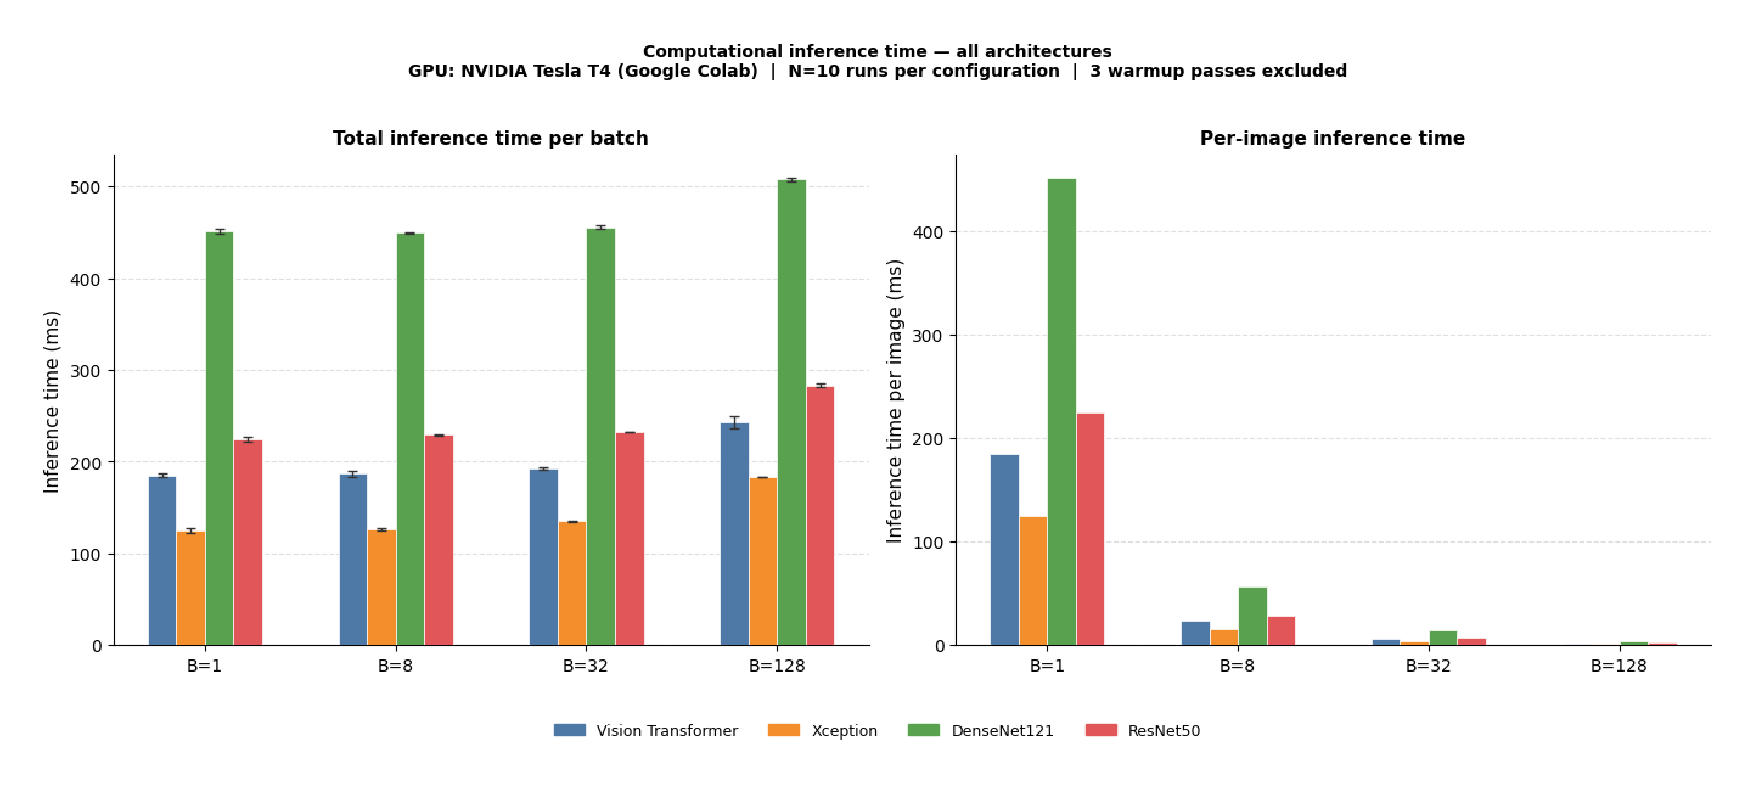
\includegraphics[width=\linewidth]{inference}
    \caption{Inference latency comparison across the 
    four regression architectures on an NVIDIA H100 
    GPU (Google Colab Pro) for batch sizes 
    $B \in \{1, 8, 32, 128\}$. Each bar reports the 
    mean $\pm$ standard deviation over $N=10$ forward 
    passes (3 warmup passes excluded). 
    \textbf{(a)} Total batch processing latency 
    in milliseconds. \textbf{(b)} Per-image latency 
    in ms/image, illustrating the amortization of 
    GPU overhead across parallel samples. Xception 
    achieves the lowest per-image latency in both 
    the single-sample ($127.71$~ms) and batch 
    ($1.47$~ms) regimes. The Vision Transformer 
    exhibits competitive batch throughput at $B=128$ 
    ($1.92$~ms/image), with a factor of only 
    $1.31\times$ overhead relative to Xception, 
    despite its $4.1\times$ larger parameter count.}
    \label{fig:inference_times}
\end{figure*}

Taken together, the computational analysis establishes 
a clear and physically motivated architecture selection 
criterion for the inverse Hamiltonian estimation task. 
For real-time single-image applications, Xception 
provides the optimal balance of inference speed 
($127.71$~ms/image) and regression accuracy, ranking 
second overall in predictive performance. For 
high-throughput batch processing pipelines, the Vision 
Transformer is the preferred architecture: its superior 
predictive performance (Section~\ref{sec:dl_results}) 
is achieved at a marginal throughput cost of $1.31\times$ 
relative to Xception at $B=128$, and its higher training 
cost is a one-time investment that need not be repeated 
at inference time. These results demonstrate that the 
proposed RAMs-based interpretability framework is 
computationally tractable for practical materials 
characterization scenarios, requiring sub-2~ms per image 
for both the best-performing architectures in the batch 
regime.


\subsection{Limitations}
\label{sec:limitations}

Despite the promising results demonstrated across the 
regression, clustering, and interpretability analyses, 
the proposed framework presents several inherent 
limitations that must be explicitly acknowledged to 
contextualize its applicability and guide future 
research directions.

The most fundamental limitation of the framework is the intrinsic
partial observability of the extended Heisenberg Hamiltonian from
two-dimensional magnetization images. As established in
Section~\ref{sec:dl_results} and confirmed by the
RAM-based interpretability analysis of
Section~\ref{sec:rams_results}, the projection of the
three-dimensional spin configuration onto the out-of-plane component
$s_z$ of the central layer of the nanodot constitutes a
dimensionality reduction that irreversibly discards physical
information. The magnetocrystalline anisotropy constants
$\tilde{K}_{an1}$ and $\tilde{K}_{anS}$, the external Zeeman field
$\tilde{H}_{ex}$, and the higher-order exchange constants
$\tilde{J}_3$ and $\tilde{J}_4$ produce spatially degenerate
magnetization signatures in the $s_z$ projection that cannot be
fully disentangled by any purely image-based regression model,
regardless of its capacity or architecture. Two distinct
observational constraints contribute to this limitation. First, the
anisotropy and Zeeman parameters couple primarily to the in-plane
spin components $s_x$ and $s_y$ rather than to $s_z$, so they are
recoverable only indirectly through the secondary topological
imprints they induce on the chiral domain structure. Second, the
input images are extracted exclusively from the central discrete
layer ($z = \lfloor \breve{L}/2 \rfloor$) of the three-dimensional
nanodot lattice, discarding the depth-resolved spin structure that
encodes the surface-to-bulk anisotropy ratio
$\tilde{K}_{anS}/\tilde{K}_{an1}$ and the conical tilt angle of
helical spin textures. Recovering these parameters with high
fidelity would therefore require either access to the full
three-dimensional spin vector field $\mathbf{S}_i = (s_x, s_y, s_z)$
at each lattice site, or volumetric magnetization inputs obtained
through multi-layer or tomographic magnetic imaging techniques. This
is not a limitation of the deep learning models themselves but of
the observational modality assumed by the framework, which mimics
the two-dimensional projection inherent to most experimental
magnetic imaging techniques such as magnetic force microscopy or
Lorentz transmission electron microscopy.

The dataset utilized in this study consists entirely 
of simulated magnetization images generated through 
the atomistic Monte Carlo framework described in 
Section~\ref{sec:montecarlo_sim}. While the 
simulation protocol incorporates physically realistic 
finite-size effects, cylindrical boundary conditions, 
and thermodynamic relaxation via simulated annealing, 
it does not account for several experimental 
phenomena that are routinely present in real magnetic 
nanodot imaging. These include thermal noise and 
instrument-specific point spread functions inherent 
to the imaging apparatus, crystallographic defects, 
vacancies, and grain boundaries that break the 
assumed periodic lattice symmetry, surface 
reconstruction effects that modify the effective 
exchange and DMI parameters at the physical boundary 
of the nanodot, and substrate-induced strain fields 
that can renormalize the bulk Hamiltonian parameters. 
As a consequence, a model trained exclusively on 
simulated data may exhibit significant performance 
degradation when applied to experimentally acquired 
magnetization images --- a domain shift problem 
that has not been quantified in the present work. 
Bridging this simulation-to-experiment gap would 
require either transfer learning with a small set 
of experimentally labeled samples or the 
incorporation of physics-informed data augmentation 
strategies that realistically replicate experimental 
noise sources.

Although the dataset encompasses 218{,}256 simulated 
configurations spanning a broad range of Hamiltonian 
parameters, the sampling strategy employed --- 
uniform random sampling within the parameter 
bounds --- does not guarantee uniform coverage of 
the magnetic phase space. As evidenced by the UMAP 
clustering analysis of Section~\ref{sec:dl_results}, 
the latent space exhibits strongly non-uniform 
density: the Labyrinthine \& Conical and Helical 
phases, which require precise combinations of 
$\tilde{K}_{DM}$ and $T^{(0)}$, are substantially 
overrepresented relative to the Ferromagnetic phase, 
which occupies a disproportionately small region of 
the parameter space. This imbalance propagates 
directly into the regression performance: the models 
achieve higher accuracy for phases with greater 
dataset density, while underperforming in 
topologically marginal regimes such as the 
ferromagnetic-to-skyrmion phase boundary where 
the mapping from parameters to magnetization 
textures is most degenerate.

From a deep learning perspective, the RAM-based 
interpretability framework introduced in this work 
provides spatially resolved gradient attributions 
that are physically consistent and architecturally 
agnostic. However, RAMs share the fundamental 
limitations of all gradient-based saliency methods: 
the attribution maps reflect the local sensitivity 
of the objective function $\mathcal{O}_p$ to spatial 
activations at the point of evaluation, but do not 
provide a globally faithful explanation of the 
model's decision function across the full parameter 
space. In particular, gradient saturation in deeply 
nonlinear networks can produce spatially diffuse 
or spurious attributions for parameters with low 
predictive signal --- precisely the degenerate 
parameters identified in this study. Furthermore, 
the current RAM formulation computes a single 
attribution map per image per parameter, which 
does not capture the stochastic uncertainty in 
the attribution due to the non-deterministic 
elements of the forward pass. Future extensions 
could incorporate ensemble-based or Bayesian 
attribution methods to provide confidence intervals 
on the spatial interpretability maps, which would 
be particularly valuable for the physically 
ambiguous parameter--phase combinations identified 
in Section~\ref{sec:rams_results}.

While the inference latency of the regression models 
is highly competitive --- sub-2~ms per image at 
batch size $B=128$ for both the Vision Transformer 
and Xception --- the computation of Regression 
Activation Maps introduces a substantial additional 
overhead. Each RAM requires a forward pass, a 
backward pass through the gradient tape, and a 
spatial upsampling operation, increasing the 
per-image computational cost by approximately one 
to two orders of magnitude relative to standard 
inference. For the Vision Transformer, which 
requires constructing a \texttt{tf.Variable} over 
the $N_r = 196$ token embeddings and differentiating 
through the GlobalAveragePooling and Dense layers, 
this overhead is particularly pronounced. 
Consequently, the full RAMs pipeline is better 
suited to offline post-hoc analysis of selected 
samples rather than real-time interpretability 
during high-throughput characterization. 
Approximation strategies such as layer-wise 
relevance propagation or integrated gradients 
computed on compressed token representations could 
reduce this overhead while preserving the physical 
interpretability of the attribution maps.

\section{Conclusions}
\label{sec:conclusions}

This work introduced a regression-based explainable deep learning
framework for the inverse estimation of Hamiltonian parameters from
two-dimensional magnetization images of magnetic nanodots. The
proposed methodology integrates atomistic Monte Carlo simulations
under a physically rigorous extended Heisenberg Hamiltonian with eight
free parameters, five state-of-the-art deep learning architectures, an
unsupervised latent space analysis via UMAP and density-based
clustering, and a novel spatial interpretability formulation RAMs that generalizes gradient-based
activation mapping to the continuous regression domain for both
convolutional and transformer-based architectures.
 
Among the five evaluated architectures, the Vision Transformer
achieved the highest overall regression accuracy across all eight
Hamiltonian parameters, followed by Xception as the best-performing
CNN baseline. Both models demonstrated strong predictive capability
for the thermodynamic temperature $T^{(0)}$, the second-shell exchange
constant $\tilde{J}_2$, and the DMI
strength $\tilde{K}_{DM}$, which constitute the physically dominant
parameters governing the observable spin texture in the $s_z$
projection. By contrast, the magnetocrystalline anisotropy constants
$\tilde{K}_{an1}$ and $\tilde{K}_{anS}$, the external Zeeman field
$\tilde{H}_{ex}$, and the higher-order exchange constants
$\tilde{J}_3$ and $\tilde{J}_4$ exhibited systematically low
identifiability across all architectures, with near-zero or undefined
$R^2$ values. This result establishes that the fundamental limitation
of the inverse problem is not architectural capacity but the intrinsic
partial observability of the extended Hamiltonian from the
two-dimensional $s_z$ projection --- a physical constraint that cannot
be overcome by increasing model complexity.
 
Beyond the aggregate regression performance, the UMAP projection of
the Vision Transformer's latent representations revealed that the
model has autonomously organized the magnetization textures into
geometrically distinct and physically interpretable regions of the
embedding space, without any explicit supervision of magnetic phase
labels. Density-based clustering of this embedding identified four
dominant magnetic phase categories: Ferromagnetic, Skyrmions and
Others, Labyrinthine \& Conical, and Helical. The per-phase regression
analysis confirmed that the model achieves its highest accuracy within
the ordered low-temperature phases --- Labyrinthine \& Conical
($R^2 = 0.978$ for $T^{(0)}$, $R^2 = 0.970$ for $\tilde{K}_{DM}$) and
Helical ($R^2 = 0.968$ for $T^{(0)}$, $R^2 = 0.866$ for
$\tilde{K}_{DM}$) --- where the magnetization texture carries the most
discriminative physical information. These results demonstrate that
the Vision Transformer's global self-attention mechanism effectively
encodes the long-range spin correlations characteristic of
topologically ordered magnetic phases.
 
The proposed RAMs formulation successfully
extended gradient-based activation mapping to the continuous
regression setting through a scale-invariant Gaussian error-decay
objective $\mathcal{O}_p = \exp(-\gamma_p(\theta_p -
\hat{\theta}_p)^2)$, providing physically interpretable spatial
attribution maps for each Hamiltonian parameter independently. For the
Xception architecture, the layer-resolved RAM analysis revealed a
physically consistent hierarchical decoupling across network depth:
early entry-flow layers (\texttt{block1}, \texttt{block3}) capture
fine-grained domain periodicity and chiral winding angles at high
spatial resolution, while deeper middle-flow and exit-flow layers
(\texttt{block8}--\texttt{block13}) consolidate these local features
into coarser, topologically meaningful representations of the global
magnetic phase. For the Vision Transformer, the patch-level RAM
attributions derived from the reshaped token embedding
$\mathbf{A}_{\text{ViT}} \in \mathbb{R}^{14 \times 14 \times 768}$
exhibited smooth, globally coherent spatial patterns that concentrated
on chiral domain walls and stripe boundaries in the ordered phases,
and produced sparse, peripheral activations for physically degenerate
parameter--phase combinations. Critically, both architectures
identified the same set of physically meaningful spatial features as
the primary drivers of accurate regression, confirming that the
learned representations are physically grounded rather than
statistically arbitrary, and both failed to produce spatially
concentrated activations for the non-identifiable parameters,
providing a direct, architecture-agnostic validation of the
identifiability hierarchy.
 
From a deployment standpoint, the inference latency analysis
demonstrated that the proposed framework is computationally viable for
practical materials characterization workflows. Xception achieves the
lowest per-image latency in both the single-sample ($127.71$~ms) and
batch ($1.47$~ms at $B = 128$) regimes, while the Vision Transformer
achieves competitive batch throughput at $1.92$~ms/image at $B = 128$
--- a factor of only $1.31\times$ slower than Xception despite its
$4.1\times$ larger parameter count. These results establish that the
Vision Transformer is the preferred architecture for high-throughput
batch characterization pipelines, where its superior regression
accuracy is achieved at a negligible throughput cost relative to the
best CNN baseline.
 
Taken together, the results of this study demonstrate that
regression-based deep learning, combined with physically motivated
interpretability methods, constitutes a viable and physically
meaningful approach to the inverse Hamiltonian estimation problem in
magnetic nanostructures. The proposed RAMs framework is
architecture-agnostic and directly applicable to any continuous
regression task where spatial attribution of physical parameters is
required, extending beyond magnetic nanodots to other physical systems
characterized by spatially resolved imaging modalities.
 
Several directions merit investigation in future work. First,
incorporating the full three-dimensional spin vector field
$\mathbf{S}_i = (s_x, s_y, s_z)$ or multi-layer volumetric
magnetization images as input would substantially reduce the partial
observability constraint and improve the identifiability of the
anisotropy and field parameters. Second, domain adaptation strategies, including physics-informed data augmentation and few-shot transfer
learning from experimentally labeled samples, are necessary to
bridge the simulation-to-experiment gap and enable direct application
to real magnetic imaging data. Third, extending the RAM formulation to
incorporate uncertainty quantification through ensemble-based or
Bayesian attribution methods would provide confidence intervals on the
spatial interpretability maps, which are particularly valuable for
physically ambiguous parameter--phase combinations near topological
phase boundaries. Finally, the integration of the proposed framework
with active learning strategies, where the model identifies the
most informative parameter combinations to simulate next, could
dramatically accelerate the construction of training datasets for
high-dimensional Hamiltonian spaces, enabling the extension of the
inverse estimation approach to more complex magnetic systems with
larger numbers of competing energetic contributions.


\section*{Acknowledgments}
Under grants provided by the research project: "Aprendizaje automático aplicado a la predicción eficiente de propiedades magnéticas de nanopartículas como soporte a la generación de dispositivos electrónicos" Hermes 62642, funded by Universidad Nacional de Colombia. Also, A. Alvarez thanks to the project: "Estimación de la capacidad de generación de energía eléctrica del agua coproducida en campos de petróleo y gas en Colombia a partir de técnicas de aprendizaje automático informado por la física," Code 111908, funded by 951-2024 Convocatoria fortalecimiento del conocimiento científico y tecnológico de las fuentes - Minciencias.ñkm

\section*{Declaration of generative AI and AI-assisted technologies in the manuscript preparation process}

During the preparation of this work the author(s) used Gemini and Claude in order to enhance the writing style. After using this tool/service, the author(s) reviewed and edited the content as needed and take(s) full responsibility for the content of the published article.



%% Loading bibliography style file
%\bibliographystyle{model1-num-names}
%\bibliographystyle{cas-model2-names}
\bibliographystyle{ieeetr}

% Loading bibliography database
\begin{thebibliography}{10}

\bibitem{heinrich2021quantum}
A.~J. Heinrich, W.~D. Oliver, L.~M. Vandersypen, A.~Ardavan, R.~Sessoli, D.~Loss, A.~B. Jayich, J.~Fernandez-Rossier, A.~Laucht, and A.~Morello, ``Quantum-coherent nanoscience,'' {\em Nature nanotechnology}, vol.~16, no.~12, pp.~1318--1329, 2021.

\bibitem{wang2022fundamental}
K.~Wang, V.~Bheemarasetty, J.~Duan, S.~Zhou, and G.~Xiao, ``Fundamental physics and applications of skyrmions: A review,'' {\em Journal of Magnetism and Magnetic Materials}, vol.~563, p.~169905, 2022.

\bibitem{fert2024electrical}
A.~Fert, R.~Ramesh, V.~Garcia, F.~Casanova, and M.~Bibes, ``Electrical control of magnetism by electric field and current-induced torques,'' {\em Reviews of Modern Physics}, vol.~96, no.~1, p.~015005, 2024.

\bibitem{issa2013magnetic}
B.~Issa, I.~M. Obaidat, B.~A. Albiss, and Y.~Haik, ``Magnetic nanoparticles: surface effects and properties related to biomedicine applications,'' {\em International journal of molecular sciences}, vol.~14, no.~11, pp.~21266--21305, 2013.

\bibitem{charalampidis2023metadynamics}
I.~Charalampidis and J.~Barker, ``Metadynamics calculations of the effect of thermal spin fluctuations on skyrmion stability,'' {\em arXiv preprint arXiv:2310.03169}, 2023.

\bibitem{yua2017magnetic}
X.~Yua, M.~Mostovoyb, Y.~Tokunagaa, W.~Zhangc, K.~Kimotoc, Y.~Matsuic, Y.~Kanekod, N.~Nagaosaa, and Y.~Tokuraa, ``Magnetic stripes and skyrmions with helicity reversals,'' {\em PNAS}, vol.~114, no.~2, p.~E265, 2017.

\bibitem{birch2020real}
M.~Birch, D.~Cort{\'e}s-Ortu{\~n}o, L.~Turnbull, M.~Wilson, F.~Gro{\ss}, N.~Tr{\"a}ger, A.~Laurenson, N.~Bukin, S.~Moody, M.~Weigand, {\em et~al.}, ``Real-space imaging of confined magnetic skyrmion tubes,'' {\em Nature communications}, vol.~11, no.~1, p.~1726, 2020.

\bibitem{yu2021magnetic}
X.~Yu, ``Magnetic imaging of various topological spin textures and their dynamics,'' {\em Journal of Magnetism and Magnetic Materials}, vol.~539, p.~168332, 2021.

\bibitem{zhang2023magnetic}
H.~Zhang, Y.~Zhang, Z.~Hou, M.~Qin, X.~Gao, and J.~Liu, ``Magnetic skyrmions: materials, manipulation, detection, and applications in spintronic devices,'' {\em Materials Futures}, vol.~2, no.~3, p.~032201, 2023.

\bibitem{tokura2020magnetic}
Y.~Tokura and N.~Kanazawa, ``Magnetic skyrmion materials,'' {\em Chemical Reviews}, vol.~121, no.~5, pp.~2857--2897, 2020.

\bibitem{zelent2023stabilization}
M.~Zelent, M.~Moalic, M.~Mruczkiewicz, X.~Li, Y.~Zhou, and M.~Krawczyk, ``Stabilization and racetrack application of asymmetric n{\'e}el skyrmions in hybrid nanostructures,'' {\em Scientific Reports}, vol.~13, no.~1, p.~13572, 2023.

\bibitem{rohart2013skyrmion}
S.~Rohart and A.~Thiaville, ``Skyrmion confinement in ultrathin film nanostructures in the presence of dzyaloshinskii-moriya interaction,'' {\em Physical Review B—Condensed Matter and Materials Physics}, vol.~88, no.~18, p.~184422, 2013.

\bibitem{kong2023quantifying}
J.~F. Kong, Y.~Ren, M.~N. Tey, P.~Ho, K.~H. Khoo, X.~Chen, and A.~Soumyanarayanan, ``Quantifying the magnetic interactions governing chiral spin textures using deep neural networks,'' {\em ACS Applied Materials \& Interfaces}, vol.~16, no.~1, pp.~1025--1032, 2023.

\bibitem{evans2014atomistic}
R.~F. Evans, W.~J. Fan, P.~Chureemart, T.~A. Ostler, M.~O. Ellis, and R.~W. Chantrell, ``Atomistic spin model simulations of magnetic nanomaterials,'' {\em Journal of Physics: Condensed Matter}, vol.~26, no.~10, p.~103202, 2014.

\bibitem{aldarawsheh2023intrinsic}
A.~Aldarawsheh, M.~Sallermann, M.~Abusaa, and S.~Lounis, ``Intrinsic n{\'e}el antiferromagnetic multimeronic spin textures in ultrathin films,'' {\em The journal of physical chemistry letters}, vol.~14, no.~40, pp.~8970--8978, 2023.

\bibitem{finocchio2016magnetic}
G.~Finocchio, F.~B{\"u}ttner, R.~Tomasello, M.~Carpentieri, and M.~Kl{\"a}ui, ``Magnetic skyrmions: from fundamental to applications,'' {\em Journal of Physics D: Applied Physics}, vol.~49, no.~42, p.~423001, 2016.

\bibitem{back20202020}
C.~Back, V.~Cros, H.~Ebert, K.~Everschor-Sitte, A.~Fert, M.~Garst, T.~Ma, S.~Mankovsky, T.~Monchesky, M.~Mostovoy, {\em et~al.}, ``The 2020 skyrmionics roadmap,'' {\em Journal of Physics D: Applied Physics}, vol.~53, no.~36, p.~363001, 2020.

\bibitem{he2023ferroelectrically}
Z.~He, W.~Du, K.~Dou, Y.~Dai, B.~Huang, and Y.~Ma, ``Ferroelectrically tunable magnetic skyrmions in two-dimensional multiferroics,'' {\em Materials Horizons}, vol.~10, no.~9, pp.~3450--3457, 2023.

\bibitem{murakami2022inverse}
R.~Murakami, M.~Mizumaki, I.~Akai, and H.~Shouno, ``Inverse estimation of parameters for the magnetic domain via dynamics matching using visual-perceptive similarity,'' {\em Science and Technology of Advanced Materials: Methods}, vol.~2, no.~1, pp.~139--152, 2022.

\bibitem{kwon2020magnetic}
H.~Y. Kwon, H.~Yoon, C.~Lee, G.~Chen, K.~Liu, A.~Schmid, Y.~Wu, J.~Choi, and C.~Won, ``Magnetic hamiltonian parameter estimation using deep learning techniques,'' {\em Science advances}, vol.~6, no.~39, p.~eabb0872, 2020.

\bibitem{nguyen2022cooperative}
T.~N.~H. Nguyen, L.~Rasabathina, O.~Hellwig, A.~Sharma, G.~Salvan, S.~Yochelis, Y.~Paltiel, L.~T. Baczewski, and C.~Tegenkamp, ``Cooperative effect of electron spin polarization in chiral molecules studied with non-spin-polarized scanning tunneling microscopy,'' {\em ACS applied materials \& interfaces}, vol.~14, no.~33, pp.~38013--38020, 2022.

\bibitem{zhao2025overview}
J.~Zhao, L.~Bai, S.~Li, Z.~Cao, Y.~Peng, J.~Bai, X.~Cai, X.~Shi, X.~Lin, G.~Wei, {\em et~al.}, ``An overview of advanced instruments for magnetic characterization and measurements,'' {\em Frontiers in Electronics}, vol.~6, p.~1645594, 2025.

\bibitem{gaida2023lorentz}
J.~H. Gaida, H.~Louren{\c{c}}o-Martins, S.~V. Yalunin, A.~Feist, M.~Sivis, T.~Hohage, F.~J. Garc{\'\i}a~de Abajo, and C.~Ropers, ``Lorentz microscopy of optical fields,'' {\em Nature Communications}, vol.~14, no.~1, p.~6545, 2023.

\bibitem{d2023micromagnetic}
M.~d'Aquino, S.~Perna, M.~Pancaldi, R.~Hertel, S.~Bonetti, and C.~Serpico, ``Micromagnetic study of inertial spin waves in ferromagnetic nanodots,'' {\em Physical Review B}, vol.~107, no.~14, p.~144412, 2023.

\bibitem{lepadatu2021micromagnetic}
S.~Lepadatu, ``Micromagnetic monte carlo method with variable magnetization length based on the landau--lifshitz--bloch equation for computation of large-scale thermodynamic equilibrium states,'' {\em Journal of Applied Physics}, vol.~130, no.~16, 2021.

\bibitem{yin2023computational}
X.~Yin, {\em Computational Materials Design: Integrating Physics With Optimization and Machine Learning}.
\newblock PhD thesis, Carnegie Mellon University, 2023.

\bibitem{karnatov2025analysis}
S.~Karnatov, ``Analysis of psnr, ssim, lpips metrics in the context of human perception of visual similarity,'' {\em Transport systems and technologies}, no.~46, 2025.

\bibitem{lee2024deep}
W.~S. Lee, T.~Song, and K.-M. Kim, ``Deep learning methods for hamiltonian parameter estimation and magnetic domain image generation in twisted van der waals magnets,'' {\em Machine Learning: Science and Technology}, vol.~5, no.~2, p.~025073, 2024.

\bibitem{chen2024data}
Y.~Chen, Q.~Yang, Y.~Li, H.~Zhang, and C.~Zhang, ``Data-driven deep convolutional neural networks for electromagnetic field estimation of transformers,'' {\em IEEE Transactions on Applied Superconductivity}, vol.~34, no.~8, pp.~1--5, 2024.

\bibitem{lan2022scaling}
S.~Lan, S.~Li, and B.~Shahbaba, ``Scaling up bayesian uncertainty quantification for inverse problems using deep neural networks,'' {\em SIAM/ASA Journal on Uncertainty Quantification}, vol.~10, no.~4, pp.~1684--1713, 2022.

\bibitem{huang2023cycle}
L.~Huang, J.~Li, X.~Ding, Y.~Zhang, H.~Chen, and A.~Ozcan, ``Cycle-consistency-based uncertainty quantification of neural networks in inverse imaging problems,'' {\em Intelligent Computing}, vol.~2, p.~0071, 2023.

\bibitem{baldan2023physics}
M.~Baldan, P.~Di~Barba, and D.~A. Lowther, ``Physics-informed neural networks for inverse electromagnetic problems,'' {\em IEEE Transactions on Magnetics}, vol.~59, no.~5, pp.~1--5, 2023.

\bibitem{wang2021learning}
W.~Wang, Z.~Wang, Y.~Zhang, B.~Sun, and K.~Xia, ``Learning order parameters from videos of skyrmion dynamical phases with neural networks,'' {\em Physical Review Applied}, vol.~16, no.~1, p.~014005, 2021.

\bibitem{vcadevz2026neural}
T.~{\v{C}}ade{\v{z}} and K.-M. Kim, ``Neural scaling laws for deep regression on domain image data of twisted magnets,'' {\em Machine Learning: Science and Technology}, vol.~7, no.~2, p.~025011, 2026.

\bibitem{he2022survey}
M.~He, B.~Li, and S.~Sun, ``A survey of class activation mapping for the interpretability of convolution neural networks,'' in {\em International Conference On Signal And Information Processing, Networking And Computers}, pp.~399--407, Springer, 2022.

\bibitem{zeng2022direct}
J.~Zeng, M.~Albooyeh, M.~Rajaei, A.~A. Sifat, E.~O. Potma, H.~K. Wickramasinghe, and F.~Capolino, ``Direct detection of photoinduced magnetic force at the nanoscale reveals magnetic nearfield of structured light,'' {\em Science advances}, vol.~8, no.~45, p.~eadd0233, 2022.

\bibitem{altaf2024applications}
A.~Altaf, M.~Shakir, H.~A. Irshad, S.~Atif, U.~Kumari, O.~Islam, W.~T. Kimberly, E.~Knopp, C.~Truwit, K.~Siddiqui, {\em et~al.}, ``Applications, limitations and advancements of ultra-low-field magnetic resonance imaging: a scoping review,'' {\em Surgical neurology international}, vol.~15, p.~218, 2024.

\bibitem{silva2024three}
G.~A. Silva, A.~Bergeron, J.~Plascak, and D.~Landau, ``Three-dimensional heisenberg model with dzyaloshinskii-moriya interaction: A monte carlo study,'' {\em Physical Review E}, vol.~109, no.~6, p.~064113, 2024.

\bibitem{mongwe2021adaptive}
W.~T. Mongwe, R.~Mbuvha, and T.~Marwala, ``Adaptive magnetic hamiltonian monte carlo,'' {\em IEEE Access}, vol.~9, pp.~152993--153003, 2021.

\bibitem{talapatra2022understanding}
A.~Talapatra, U.~Gajera, S.~P. P, J.~Arout~Chelvane, and J.~R. Mohanty, ``Understanding the magnetic microstructure through experiments and machine learning algorithms,'' {\em ACS applied materials \& interfaces}, vol.~14, no.~44, pp.~50318--50330, 2022.

\bibitem{liu2026bayesian}
M.~Liu, D.~Grana, K.~Mosegaard, M.~K. Sen, M.~Xu, and T.~Mukerji, ``Bayesian inference for subsurface geophysical inverse problems,'' {\em Reviews of Geophysics}, vol.~64, no.~1, p.~e2025RG000884, 2026.

\bibitem{zhao2023generative}
Z.~Zhao, J.~C. Ye, and Y.~Bresler, ``Generative models for inverse imaging problems: From mathematical foundations to physics-driven applications,'' {\em IEEE Signal Processing Magazine}, vol.~40, no.~1, pp.~148--163, 2023.

\bibitem{shmakov2023end}
A.~Shmakov, K.~Greif, M.~Fenton, A.~Ghosh, P.~Baldi, and D.~Whiteson, ``End-to-end latent variational diffusion models for inverse problems in high energy physics,'' {\em Advances in neural information processing systems}, vol.~36, pp.~65102--65127, 2023.

\bibitem{sui2026cyclemamba}
C.~Sui, Z.~Xu, Y.~Meng, H.~Wang, B.~Zhang, and G.~Vivone, ``Cyclemamba: Cycle-consistent learning for aerial visible-to-infrared image translation,'' {\em IEEE Transactions on Geoscience and Remote Sensing}, 2026.

\bibitem{will2021application}
A.~Will-Cole, A.~G. Kusne, P.~Tonner, C.~Dong, X.~Liang, H.~Chen, and N.~X. Sun, ``Application of bayesian optimization and regression analysis to ferromagnetic materials development,'' {\em IEEE transactions on magnetics}, vol.~58, no.~1, pp.~1--8, 2021.

\bibitem{sridharan2022modern}
B.~Sridharan, M.~Goel, and U.~D. Priyakumar, ``Modern machine learning for tackling inverse problems in chemistry: molecular design to realization,'' {\em Chemical communications}, vol.~58, no.~35, pp.~5316--5331, 2022.

\bibitem{agudelo2019study}
J.~Agudelo-Giraldo, E.~Restrepo-Parra, and D.~Landau, ``A study of magnetic domains in thin films from fm and afm interactions,'' {\em Physica A: Statistical Mechanics and its Applications}, vol.~517, pp.~542--550, 2019.

\bibitem{borisov2021heisenberg}
V.~Borisov, Y.~O. Kvashnin, N.~Ntallis, D.~Thonig, P.~Thunstr{\"o}m, M.~Pereiro, A.~Bergman, E.~Sj{\"o}qvist, A.~Delin, L.~Nordstr{\"o}m, {\em et~al.}, ``Heisenberg and anisotropic exchange interactions in magnetic materials with correlated electronic structure and significant spin-orbit coupling,'' {\em Physical Review B}, vol.~103, no.~17, p.~174422, 2021.

\bibitem{moriya1960anisotropic}
T.~Moriya, ``Anisotropic superexchange interaction and weak ferromagnetism,'' {\em Physical review}, vol.~120, no.~1, p.~91, 1960.

\bibitem{eriksson2017atomistic}
O.~Eriksson, A.~Bergman, L.~Bergqvist, and J.~Hellsvik, {\em Atomistic spin dynamics: foundations and applications}.
\newblock Oxford university press, 2017.

\bibitem{cullity2011introduction}
B.~D. Cullity and C.~D. Graham, {\em Introduction to magnetic materials}.
\newblock John Wiley \& Sons, 2011.

\bibitem{coey2010magnetism}
J.~M. Coey, {\em Magnetism and magnetic materials}.
\newblock Cambridge university press, 2010.

\bibitem{fert2017magnetic}
A.~Fert, N.~Reyren, and V.~Cros, ``Magnetic skyrmions: advances in physics and potential applications,'' {\em Nature Reviews Materials}, vol.~2, no.~7, p.~17031, 2017.

\bibitem{landau2021guide}
D.~Landau and K.~Binder, {\em A guide to Monte Carlo simulations in statistical physics}.
\newblock Cambridge university press, 2021.

\bibitem{desplat2018thermal}
L.~Desplat, D.~Suess, J.-V. Kim, and R.~L. Stamps, ``Thermal stability of metastable magnetic skyrmions: Entropic narrowing and significance of internal eigenmodes,'' {\em Physical Review B}, vol.~98, no.~13, p.~134407, 2018.

\bibitem{murphy2023probabilistic}
K.~P. Murphy, {\em Probabilistic machine learning: Advanced topics}.
\newblock MIT press, 2023.

\bibitem{koonce2021resnet}
B.~Koonce, ``Resnet 50,'' in {\em Convolutional neural networks with swift for tensorflow: image recognition and dataset categorization}, pp.~63--72, Springer, 2021.

\bibitem{huang2017densely}
G.~Huang, Z.~Liu, L.~Van Der~Maaten, and K.~Q. Weinberger, ``Densely connected convolutional networks,'' in {\em Proceedings of the IEEE conference on computer vision and pattern recognition}, pp.~4700--4708, 2017.

\bibitem{chollet2017xception}
F.~Chollet, ``Xception: Deep learning with depthwise separable convolutions,'' in {\em Proceedings of the IEEE conference on computer vision and pattern recognition}, pp.~1251--1258, 2017.

\bibitem{dosovitskiy2020image}
A.~Dosovitskiy, L.~Beyer, A.~Kolesnikov, D.~Weissenborn, X.~Zhai, T.~Unterthiner, M.~Dehghani, M.~Minderer, G.~Heigold, S.~Gelly, {\em et~al.}, ``An image is worth 16x16 words: Transformers for image recognition at scale,'' {\em arXiv preprint arXiv:2010.11929}, 2020.

\bibitem{vinogradova2020gradcam}
K.~Vinogradova, A.~Dibrov, and G.~Myers, ``Towards interpretable semantic segmentation via gradient-weighted class activation mapping (student abstract),'' in {\em Proceedings of the AAAI Conference on Artificial Intelligence}, 2020.

\bibitem{zhang2024gradcam}
Y.~Zhang, Y.~Zhu, J.~Liu, and W.~Yu, ``An interpretability optimization method for deep learning networks based on grad-cam,'' {\em IEEE}, 2024.

\bibitem{makke2024symbolic}
N.~Makke and S.~Chawla, ``Interpretable scientific discovery with symbolic regression: a review,'' {\em Applied Intelligence Review}, 2024.

\bibitem{radosavovic2023real}
I.~Radosavovic, T.~Xiao, S.~James, P.~Abbeel, J.~Malik, and T.~Darrell, ``Real-world robot learning with masked visual pre-training,'' in {\em Conference on Robot Learning}, pp.~416--426, PMLR, 2023.

\bibitem{ghojogh2021uniform}
B.~Ghojogh, A.~Ghodsi, F.~Karray, and M.~Crowley, ``Uniform manifold approximation and projection (umap) and its variants: tutorial and survey,'' {\em arXiv preprint arXiv:2109.02508}, 2021.

\end{thebibliography}



\end{document}